\section{Verbesserung der API-Usability von SeqAn}
\label{sec:seqan-api-usability-verbesserung}

Dieses Unterkapitel behandelt die erreichten API-Usability-Verbesserungen an Hand der im vorherigen Unterkapitel vorgeschlagenen Maßnahmen und wiederholt in sehr knapper Form die bereits in Phase 1 erläuterten Verbesserungen im Zuge der ersten Beseitigung grober Usability-Probleme.

Auf Grund der im gleichnamigen \hyperref[sec:schwierigkeiten]{Abschnitt erläuterten Schwierigkeiten} (S. \pageref{sec:schwierigkeiten}) konnte ich nicht für die Umsetzung aller Maßnahmen sorgen. Ganz besonders sind dabei, neben organisatorischen Gründen wie dem Wegfall von Kollegen und meiner auf drei Jahre begrenzten Stelle, wissenschaftliche Gründe, wie den Anwendungsschwierigkeiten der \gls{gtm} und dem unerwartet aufwändigen Analysewerkzeugbau, zu nennen. Aus den damit einhergehenden zeitlichen Problemen musste ich auch die im nächsten Unterkapitel vorgestellte Validierung stark kürzen.

\subsection{Prozessverbesserungen}

Im Zuge der ersten Beseitigung grober Usability-Probleme habe ich in Zusammenarbeit mit der Bioinformatik-Arbeitsgruppe die folgenden Prozessverbesserungen vorgenommen, die sich wie folgt positiv auf die Usability auswirken:
\begin{itemize}
  \item Die Einführung standardisierter Commit-Nachrichten führte zu verständlicheren und ausführlicheren Beschreibungen der Entwicklungen an SeqAn. Dies half mir als API-Evaluator die Arbeiten an SeqAn besser nachvollziehen zu können. Augenscheinlich mag dieser Schritt unwichtig wirken. Durch die hohe Dynamik in meinem Arbeitsumfeld (insb. die vielen Akteure und die stetige Fortentwicklung von SeqAn; siehe \sref{sec:rahmenbedingungen}) war diese Verbesserung jedoch von großer Wichtigkeit für mich und wirkte sich positiv auf mein Arbeitsergebnis aus.
  \item Die Umstellung von Subversion auf Git verbesserte den Entwicklungsprozess für die SeqAn-Entwickler, da sie nun lokale Revisionen erstellen konnten, ohne das zentrale Repository zu kompromittieren. Dieser Zugewinn an Freiheitsgraden erhöht die \textit{sequenzielle Vollständigkeit} der Entwicklungs-\textit{Arbeitsaufgabe}\footnote{Hierbei handelt es sich um Begriffe aus der Arbeitspsychologie. ``Eine Handlung ist sequenziell vollständig, wenn in ihr der gesamte Handlungszyklus abgedeckt ist, d.h. es kommt sowohl zu Zielbildungs-, Planungs- und Ausführungsprozessen als auch zu Kontrollprozessen.'' \citep{Bamberg:2011tv}} und damit die Wahrscheinlichkeit einer höheren Softwarequalität. Ich gehe nicht davon aus, dass ein Zugewinn an Softwarequalität zu einer Verschlechterung der API-Usability führt --- eher im Gegenteil.
  \item Die Einführung von Code-Reviews als Instrument der Qualitätssicherung verbessert ebenfalls die Softwarequalität.
\end{itemize}

Weitere Details können im \sref{sec:phase1} nachgelesen werden.



\subsection{Frameworkumbau}

SeqAn wurde erfolgreich von einem Framework zu einer Library umgebaut. Die SeqAn-Entwickler haben sämtliche Vorwärtsdeklarationen beseitigt. Fortan ist es möglich, SeqAn sowohl als Framework als auch als Library zu verwenden. Für Letzteres gibt es eine eigene Anleitung, die in allen Installationsanleitungen verlinkt ist\footnote{\url{http://seqan.readthedocs.org/en/latest/BuildManual/IntegrationWithYourOwnBuildSystem.html}}.

In Folge gibt es nun auch keine Abhängigkeiten mehr zum CMake-Build-System, der Anwender dazu zwingen könnte, den eigenen Build-Prozess umzustellen.



\subsection{STL-Angleichung}

\subsubsection{Curiously Recurring Template Pattern --- CRTP}

Ich habe das CRTP einigen SeqAn-Entwicklern zu einer Zeit präsentiert, in der ich noch in dem Glauben war, SeqAns Anwender würden eine streng objektorientierte Library erwarten. Dies entsprach zum Einen nicht den Tatsachen, denn ein großer Teil erwartete lediglich eine STL-konforme Softwarebibliothek. Zum Anderen stieß ich mit diesem Vorschlag auf Ablehnung. Ich hatte den Eindruck, dass die Idee, die SeqAn-API zu einer reinen OOP-API umzustrukturieren, für die SeqAn-Entwickler ein zu radikaler Schritt wäre.

Aus zeitlichen Gründen kam ich nicht mehr dazu, dem SeqAn-Team meinen neuen Erkenntnisstand mitzuteilen.

Die in \sref{sec:stl-inconsistencies} beschriebenen Beobachtungen lassen erwarten, dass die Umwandlung von in SeqAn globalen Funktionen, die in C\texttt{++} als Memberfunktionen implementiert wären, eine äußerst positive Auswirkung auf die Usability haben wird.

\subsubsection{Metafunktionen}

Metafunktionen werden in der SeqAn-API vornehmlich zur Berechnung von Rückgabetypen verwendet, was --- obwohl Gogol-Döring damit eine Verbesserung der Usability beabsichtigte --- tatsächlich eine Verschlechterung selbiger (siehe \code{apiua://code/-9223372036854775352}-Problem) verursachte.

Dieser Anwendungsfall ist durch das \texttt{auto}-Schlüsselwort im neuen C\texttt{++}-Sprachstandard obsolet geworden, was auch die Dynamik meines Forschungsvorhabens unterstreicht (vgl. \sref{sec:schwierigkeiten}). Mittels \texttt{auto} wird der Compiler angewiesen, den Datentyp selbstständig herzuleiten. Auf diese Weise würde man statt \mintinline{cpp}{Row<Align<String<Dna>, ArrayGaps>>::Type &row1 = row(align, 0);} nur noch \mintinline{cpp}{auto &row1 = row(align, 0);} schreiben müssen.

\subsection{KNIME als API-Endanwender-Werkzeug}

Während die STL-Angleichung die bestehende SeqAn-API an die Erwartung von C\texttt{++}-geprägten API-Anwendern annähern soll, geht es bei der Wrapper-API darum, eine zweite, speziell auf die Bedürfnisse von API-Endanwendern angepasste API zu entwickeln. Die Bereitstellung von SeqAn-Programmen innerhalb der Workflow-Engine KNIME war eines der Ziele des BioStore-Projekts (siehe Abschnitte \ref{sec:rahmenbedingungen}). Dieses Ziel haben die Bioinformatik-Arbeitsgruppe und ich wie folgt erreicht:
\begin{enumerate}
  \item KNIME-Anpassungen
  \begin{enumerate}
    \item[1.] Das von der Universität Tübingen entwickelte \textit{Common Tool Description (CTD)} Format wurde weiterentwickelt und erlaubt nun eine mächtige Beschreibung der Schnittstelle von Kommandozeilenprogrammen. Beschreibungsmöglichkeiten umfassen u.a. typisierte Argumente und Wertebereiche (vgl. \sref{sec:argument-parser}).
    \item[2.] Das ebenfalls ursprünglich an der Universität Tübingen entwickelte \textit{Generic KNIME Nodes}, wurde unter dem Namen \textit{Generic Workflow Nodes}\footnote{\url{https://github.com/genericworkflownodes}} weiterentwickelt. Es kann, unter Verwendung von CTD-Dateien, die entsprechenden Kommandozeilenprogramme als KNIME-Knoten kapseln. Diese können dann über das Internet für alle KNIME-Anwender bereitgestellt werden.
  \end{enumerate}
  \item SeqAn-Anpassungen
  \begin{enumerate}
    \item[1.] Es wurde ein neuer Parser für Argumente implementiert (siehe \sref{sec:argument-parser}).
    \begin{itemize}
      \item Der Argument-Parser ist Bestandteil der SeqAn-API und bietet mächtige Funktionen zur Beschreibung von Kommandozeilenprogrammschnittstellen.
      \item Ein Argument-Parser verwendendes SeqAn-Programm kann seine eigene Schnittstellenbeschreibung als CTD-Datei exportieren.
      \item Sämtliche SeqAn-Anwendungen (siehe \sref{sec:seqan-tools}) wurden an den Argument-Parser angepasst und verwenden diesen nun.
    \end{itemize}
    \item[2.] Die kontinuierliche Integration (engl. \textit{continuous integration --- CI}) wurde angepasst.
    \begin{itemize}
      \item Der SeqAn-CI-Server generiert nun für alle SeqAn-Anwendungen CTD-Dateien.
      \item Die SeqAn-Anwendungen werden mit Hilfe der CTD-Dateien und der Generic Workflow Nodes Anwendung zu KNIME-Knoten gepackt.
      \item Die SeqAn-KNIME-Knoten\footnote{\url{https://tech.knime.org/seqan-nodes-for-knime}} werden auf den Community-Server von KNIME hochgeladen und stehen damit allen KNIME-Anwendern zu Verfügung\footnote{\url{http://seqan.readthedocs.org/en/master/HowTo/UseSeqAnNodesInKnime.html}}.
    \end{itemize}
    \item[3.] Analog zu SeqAn-Code-Beispielen, wurden beispielhafte Workflows entwickelt\footnote{\url{https://github.com/seqan/knime_seqan_workflows}}, die in KNIME importiert werden können.
  \end{enumerate}
\end{enumerate}

Die SeqAn-Anpassungen erlauben es darüber hinaus SeqAn-Anwendern KNIME-Knoten aus ihren selbst entwickelten SeqAn-Anwendungen zu generieren.\footnote{\url{http://seqan.readthedocs.org/en/latest/HowTo/GenerateSeqAnKnimeNodes.html}}

Das Ergebnis besteht darin, dass KNIME-Anwender nun grafisch mit SeqAn arbeiten können. Dazu können SeqAn-Anwendungen in Form von Knoten auf einer KNIME-Arbeitsfläche platziert, verbunden und konfiguriert werden (siehe Abbildungen \ref{fig:knime-example} und \ref{fig:knime-config}). Auf diese Weise können API-Endanwender SeqAn-Workflows entwickeln, ohne eine einzige Zeile Code schreiben zu müssen.

\begin{figure}
  \centering
    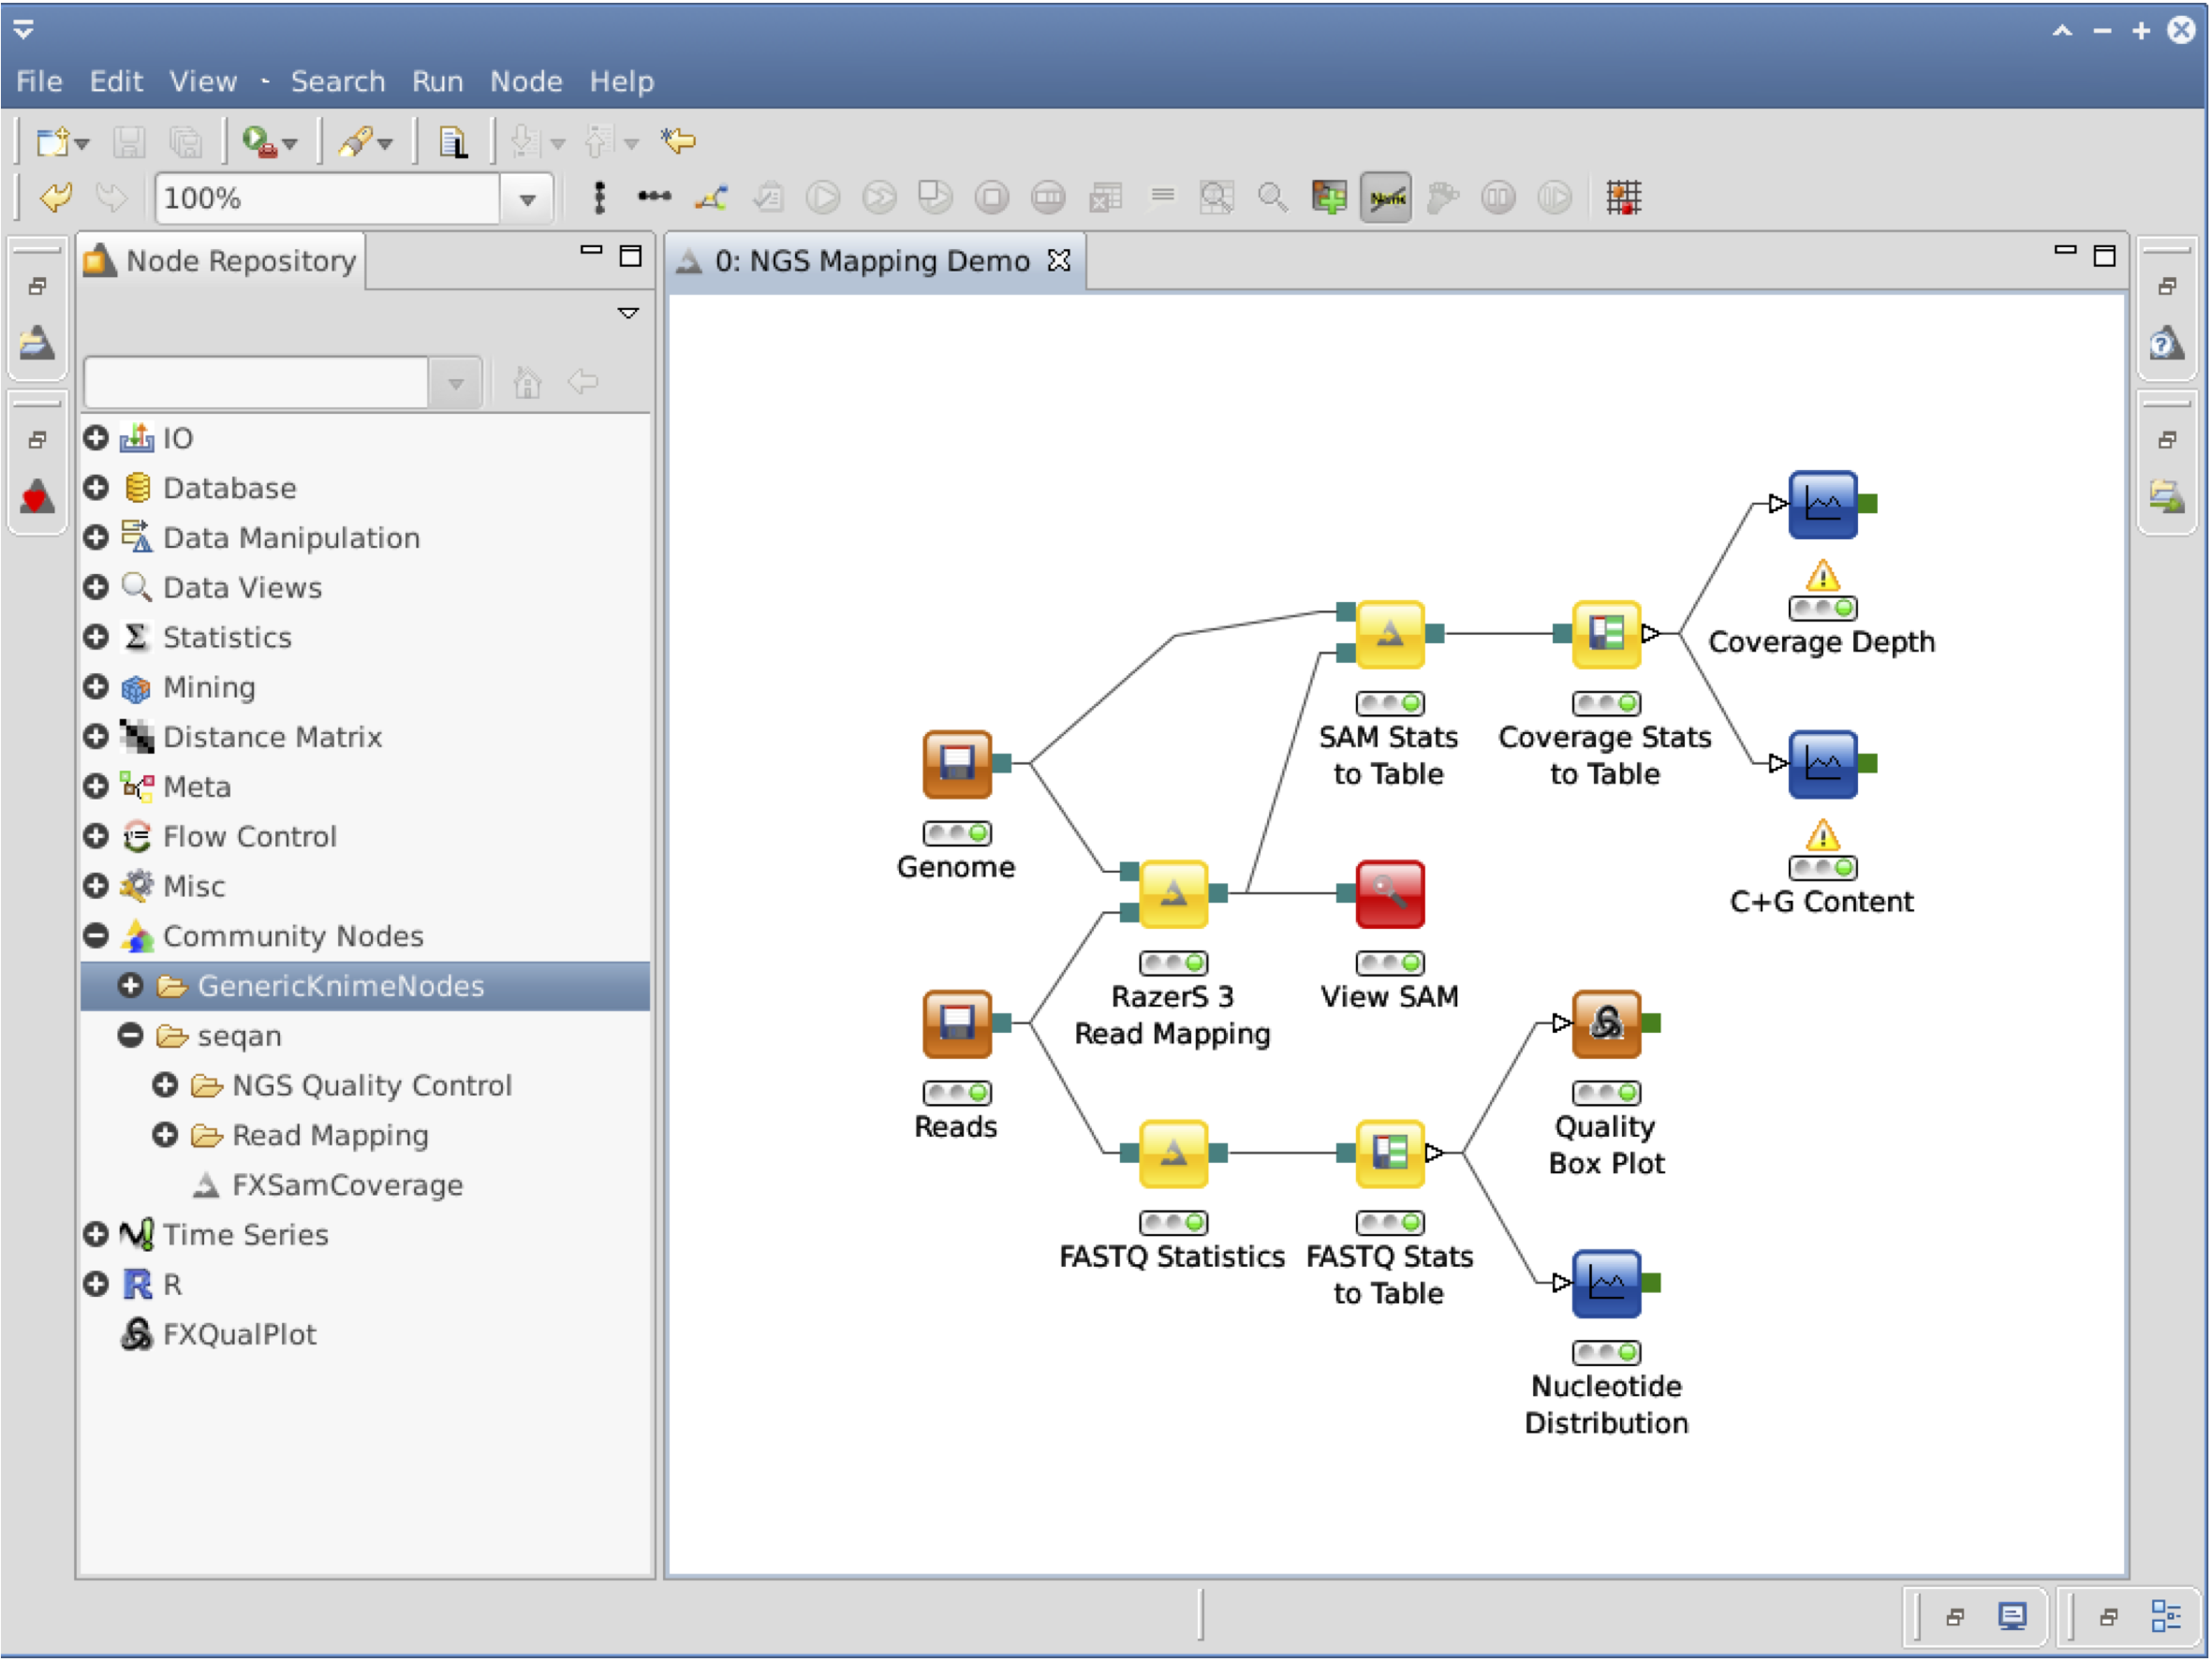
\includegraphics[width=1\linewidth]{Figures/knime-example.png}
  \caption{Beispiel-SeqAn-Workflow in KNIME}
  \label{fig:knime-example}
\end{figure}

\begin{figure}
  \centering
    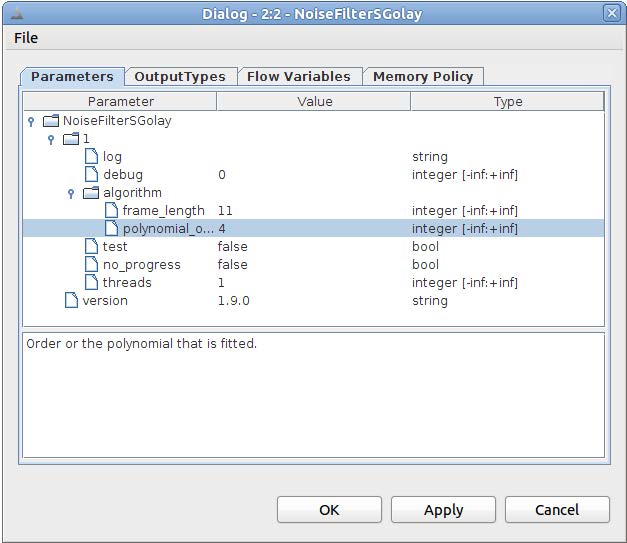
\includegraphics[width=0.65\linewidth]{Figures/knime-config.jpg}
  \caption{KNIME-Konfigurationsdialog für einen CTD-basierten Knoten}
  \label{fig:knime-config}
\end{figure}



\begin{comment}
\subsection{Intransparenzbeseitigung}

Die Fatalität des Problems der \code[apiua://code/-9223372036854775057]{versteckten Parameterübergabe} ist nicht hinreichend verstanden, um aktuell den SeqAn-Entwicklern die Problembeseitigung zu empfehlen.
\end{comment}


\subsection{Inkonsistenzbeseitigung}
\label{sec:Inkonsistenzbeseitigung}

Die Probleme \code{apiua://code/-9223372036854775116}, \code{apiua://code/-9223372036854774846} und \code{apiua://code/-9223372036854774861} wurden mit den SeqAn-Core-Entwicklern besprochen. Jedoch kam es nicht zu einer konkreten Planung zur Umsetzung dieser Maßnahme, was zwei Gründe hatte:
\begin{itemize}
  \item Zum Zeitpunkt der Vorstellung meiner Ergebnisse waren meine Lösungsvorschläge nicht konkret genug.
  \item Meine Kollegen verfolgten während der BioStore-Projektzeit genauso eigene Ziele, wie ich das mit der API-Usability-Erfoschung tat. Nach meiner Einschätzung des Standpunktes der SeqAn-Entwickler stand der Nutzen dieser Maßnahme in keinem guten Verhältnis zu den Kosten.
\end{itemize}



\subsection{Shortcuts}

Während des BioStore-Projekts, das vor einem knappen Jahr endete, konnte ich die Sensibilität für die mit den Shortcuts einhergehenden Probleme auf Seiten der SeqAn-Entwickler erhöhen. Jedoch waren meine damaligen Lösungsansätze nicht hinreichend fundiert, um die SeqAn-Entwickler zu einer Lösung der Probleme \code{apiua://code/-9223372036854774861} und \code{apiua://code/-9223372036854774860} zu bewegen.



\subsection{Fail-Fast}

Diese Maßnahme bestand aus zwei Schritten:
\begin{enumerate}
  \item Dass es Funktionen wie \texttt{length} gibt, die bei bestimmen Eingaben ungültige Rückgaben liefern, war einigen SeqAn-Entwicklern unabhängig von meinen Forschungsergebnissen bekannt. Der Entwickler Manuel Holtgrewe erachtete deren Korrektur ebenfalls für sinnvoll. Aktuell ist dieser Schritt noch nicht umgesetzt.
  \item Die Einschätzung, dass Leseoperationen Ausnahmen werfen müssen, wenn es zu einem Lesefehler kommt, teilten anfangs nur sehr wenige SeqAn-Entwickler aus Angst, SeqAn würde dadurch langsamer arbeiten. Die Notwendigkeit dieser Maßnahme und dessen Vereinbarkeit mit dem SeqAn-Entwurfsziel \textit{Performance} mittels \textit{Tags} fand zunehmend Zustimmung. Allerdings ging diese Maßnahme in den letzten Projektmonaten --- insbesondere aus Zeitgründen bei allen Beteiligten --- unter. Die Beseitigung steht also noch aus.
\end{enumerate}




\subsection{Dokumentation}
\label{sec:improve-dox}

Die SeqAn-Dokumentation besteht im weiteren Sinne aus den Installationsanleitungen, didaktischen Lernressourcen (Tutorials) und der Dokumentation selbst, die als Nachschlagewerk für SeqAn-Anwender dient.

Im Zuge der ersten Beseitigung grober Usability-Probleme habe ich gemeinsam mit meinen Kollegen bereits die Installationsanleitungen und die Tutorials umfassend überarbeitet. Die Wirksamkeit dieser Überarbeitungen habe ich bereits im \sref{sec:phase1-validierung} gezeigt. An dieser Stelle fasse ich diese Änderungen nur sehr knapp zusammen:


\subsubsection{Installationsanleitungen}

Die Installationsanleitungen waren fehlerhaft, uneinheitlich, unstrukturiert und verfügten über zu wenig Beispiele, um den Anleitungen folgen zu können. Ich habe eine inhaltliche und grafische Vorlage für alle plattformabhängigen Installationsanleitungen erstellt und dabei die folgenden Installationsanleitungsbestandteile etabliert:
\begin{enumerate}
\itemsep1pt\parskip0pt\parsep0pt
  \item Prerequisites --- Was bereits installiert sein muss + Verweise
  \item Install --- Die eigentliche SeqAn-Installation
  \item A First Build --- Überprüfung, ob Installation korrekt verlief
  \item Hello World! --- Skelett für erste eigene SeqAn-Anwendung
  \item Further Steps --- Verweise auf Dokumentation und Tutorials
\end{enumerate}

Sämtliche Installationsanleitungen wurden korrigiert und vereinheitlicht. \fref{fig:getting-started-windows2} zeigt einen Ausschnitt aus der Installationsanleitung für Windows.

\begin{figure}[ht!]
  \centering
    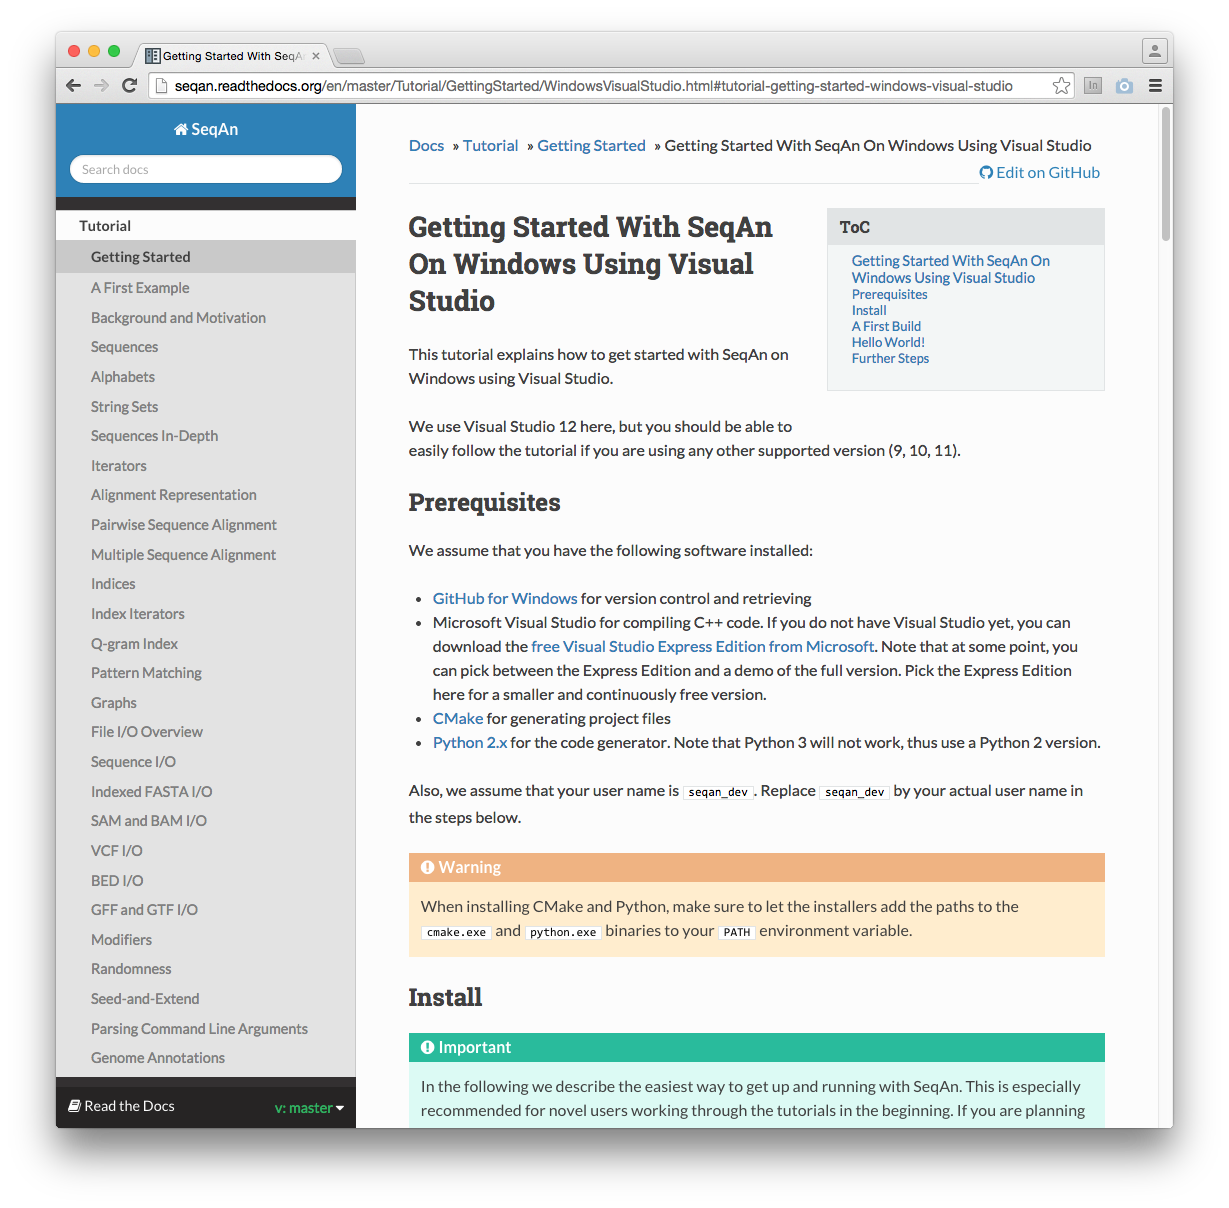
\includegraphics[width=1.0\linewidth]{Figures/getting-started-windows.png}
  \caption[SeqAn-Installation unter Windows]{Ausschnitt aus der verbesserten SeqAn-Installationsanleitung für Windows}
  \label{fig:getting-started-windows2}
\end{figure}



\subsubsection{Tutorials}

Basierend auf dem etablierten Lernphasenmodell \citep{Gagne:1985tx} und den Analyseergebnissen einer Vielzahl von Daten (Details siehe \sref{sec:phase1}) habe ich die Struktur der Tutorials überarbeitet und Qualitätskriterien formuliert. Diese Ergebnisse habe ich in Form eines Tutorials über das Schreiben von Tutorials zusammengefasst und in die Entwickler-Dokumentation integriert\footnote{\url{http://seqan.readthedocs.org/en/master/HowTo/WriteTutorials.html}}. Das Dokument richtet sich an die Autoren von SeqAn-Tutorials, wurde von diesen sehr positiv aufgenommen, gilt seitdem als verbindliche Vorlage für neue Tutorials und stellt damit einen langfristigen Beitrag für die verbesserte API-Usability von SeqAn dar.

Das Dokument besteht aus den folgenden Abschnitten:
\begin{enumerate}
\itemsep1pt\parskip0pt\parsep0pt
  \item Konventionen, die beim Verfassen von Tutorials zu beachten sind
  \item Struktur --- Aufbau eines Tutorials, explizite Metaangaben
  \item Didaktik --- Anwenderzentrierung, Übungsaufgaben
  \item Integration --- Vernetzung des Tutorials für bessere Auffindbarkeit
  \item Vorlage --- für die Erstellung eines neuen Tutorials
\end{enumerate}

Es wurden mehrere neue Tutorials durch das Auftrennen existierender Tutorials geschaffen. Besonders erwähnenswert ist dabei das neue Anfänger-Tutorial ``A First Example''\footnote{\url{http://seqan.readthedocs.org/en/master/Tutorial/FirstStepsInSeqAn.html}}, das eine besonders geringe Einstiegshürde für Anwender mit den in der \gls{gtm}-Analyse gefundenen \code[apiua://code/-9223372036854775494]{paradigmatischen Prägungen} aufweist. Es lohnt sich für den Leser dieser Dissertation das Anfänger-Tutorial einmal selbst zu öffnen.

Die Tutorials wurden sukzessive über eine längere Diskussionsphase hinweg gemeinsam von mir und den jeweiligen Autoren verbessert (siehe \fref{fig:tutorial-improved-final}) und dienen fortan als Aufgaben-bezogener SeqAn-Überblick \citep[vgl.][]{Fairbanks:2006jw,Ko:2011vw,Pugh:Ks4cicwp,Robillard:2009cs}.

\begin{figure}[ht!]
  \centering
    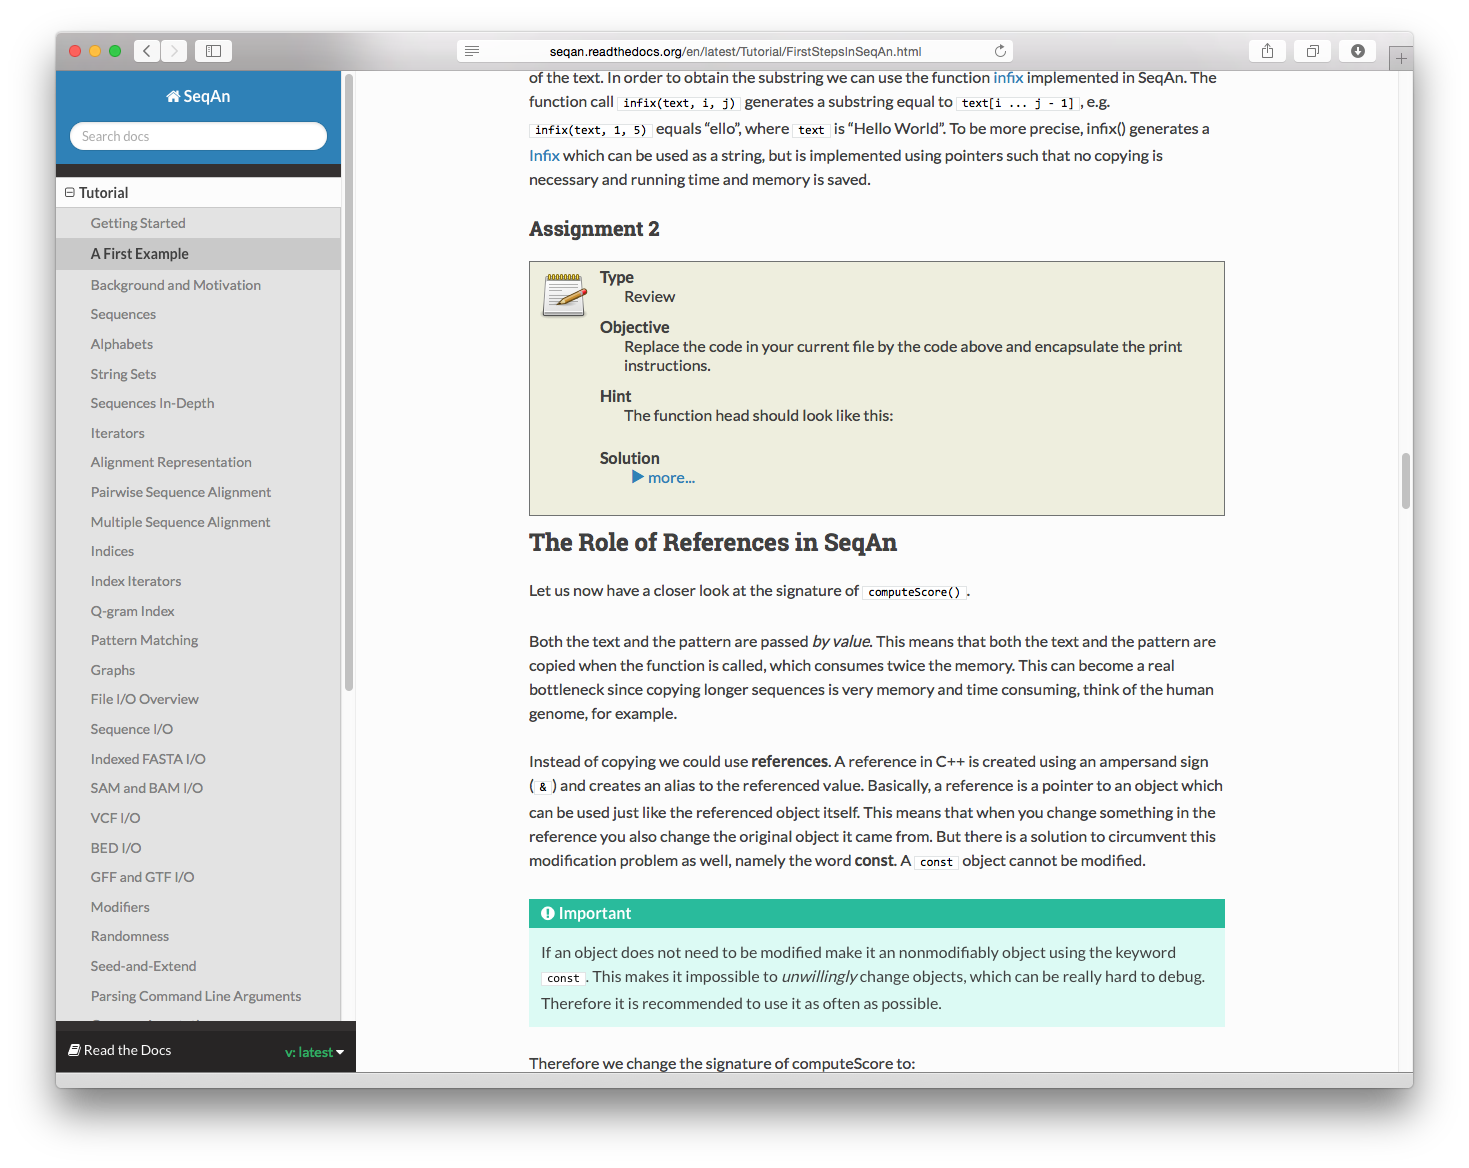
\includegraphics[width=1\linewidth]{Figures/tutorial-improved-final.png}
  \caption{Beispiel für ein überarbeitetes Tutorial}
  \label{fig:tutorial-improved-final}
\end{figure}




\subsubsection{Dokumentation}

Dokumentationen bilden ein wichtiges Bindeglied zwischen dem, was der Anwender möchte und dem, was die Library anbietet \citep{Robillard:2009cs,Kintsch:1988bz,Pennington:1987dc}. Aus diesem Grund und meinen \gls{gtm}-Analyseergebnissen habe ich die eigentliche SeqAn-Dokumentation technisch von Grund auf neu entwickelt. Die inhaltliche Überarbeitung wurde von den SeqAn-Entwicklern durchgeführt. Die \fref{fig:dox-large-all} zeigt die alte und die neue Dokumentation im Vergleich. Alternativ bietet es sich an, während des Lesens dieses Abschnitts die Dokumentation unter \href{http://docs.seqan.de/seqan/develop/}{docs.seqan.de/seqan/develop/} selbst zu öffnen.

Im Folgenden erläutere ich die Änderungen gegenüber der alten Dokumentation.

\newgeometry{inner=2cm,outer=1.5cm,top=1.5cm,bottom=1.5cm}
\thispagestyle{empty}
\begin{landscape}
\begin{figure}
        \centering
        \begin{subfigure}[b]{0.38\linewidth}
                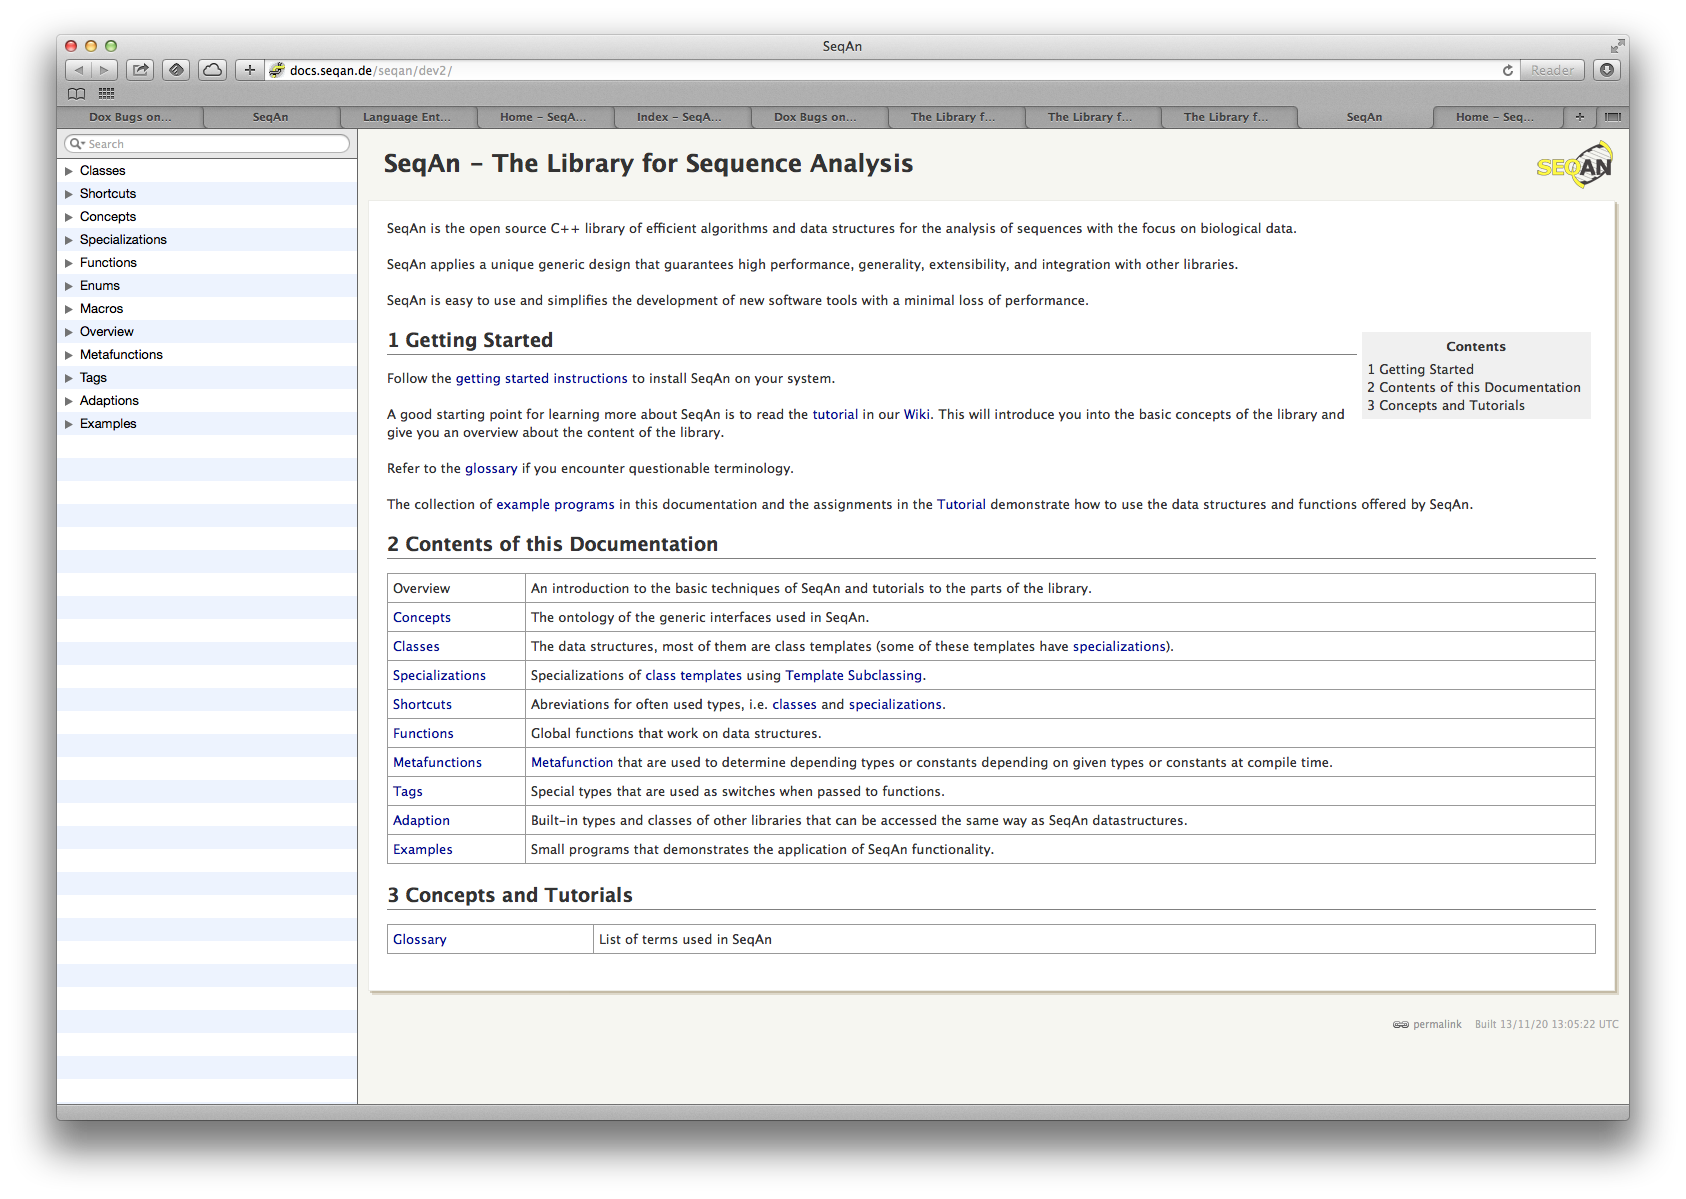
\includegraphics[width=\linewidth]{Figures/dox/dox-2_0_0-large-home.png}
                \caption{Startseite in Version 2.0.0}
                \label{fig:dox-large-home-2.0.0}
        \end{subfigure}
        \hspace{1cm}
        \begin{subfigure}[b]{0.38\linewidth}
                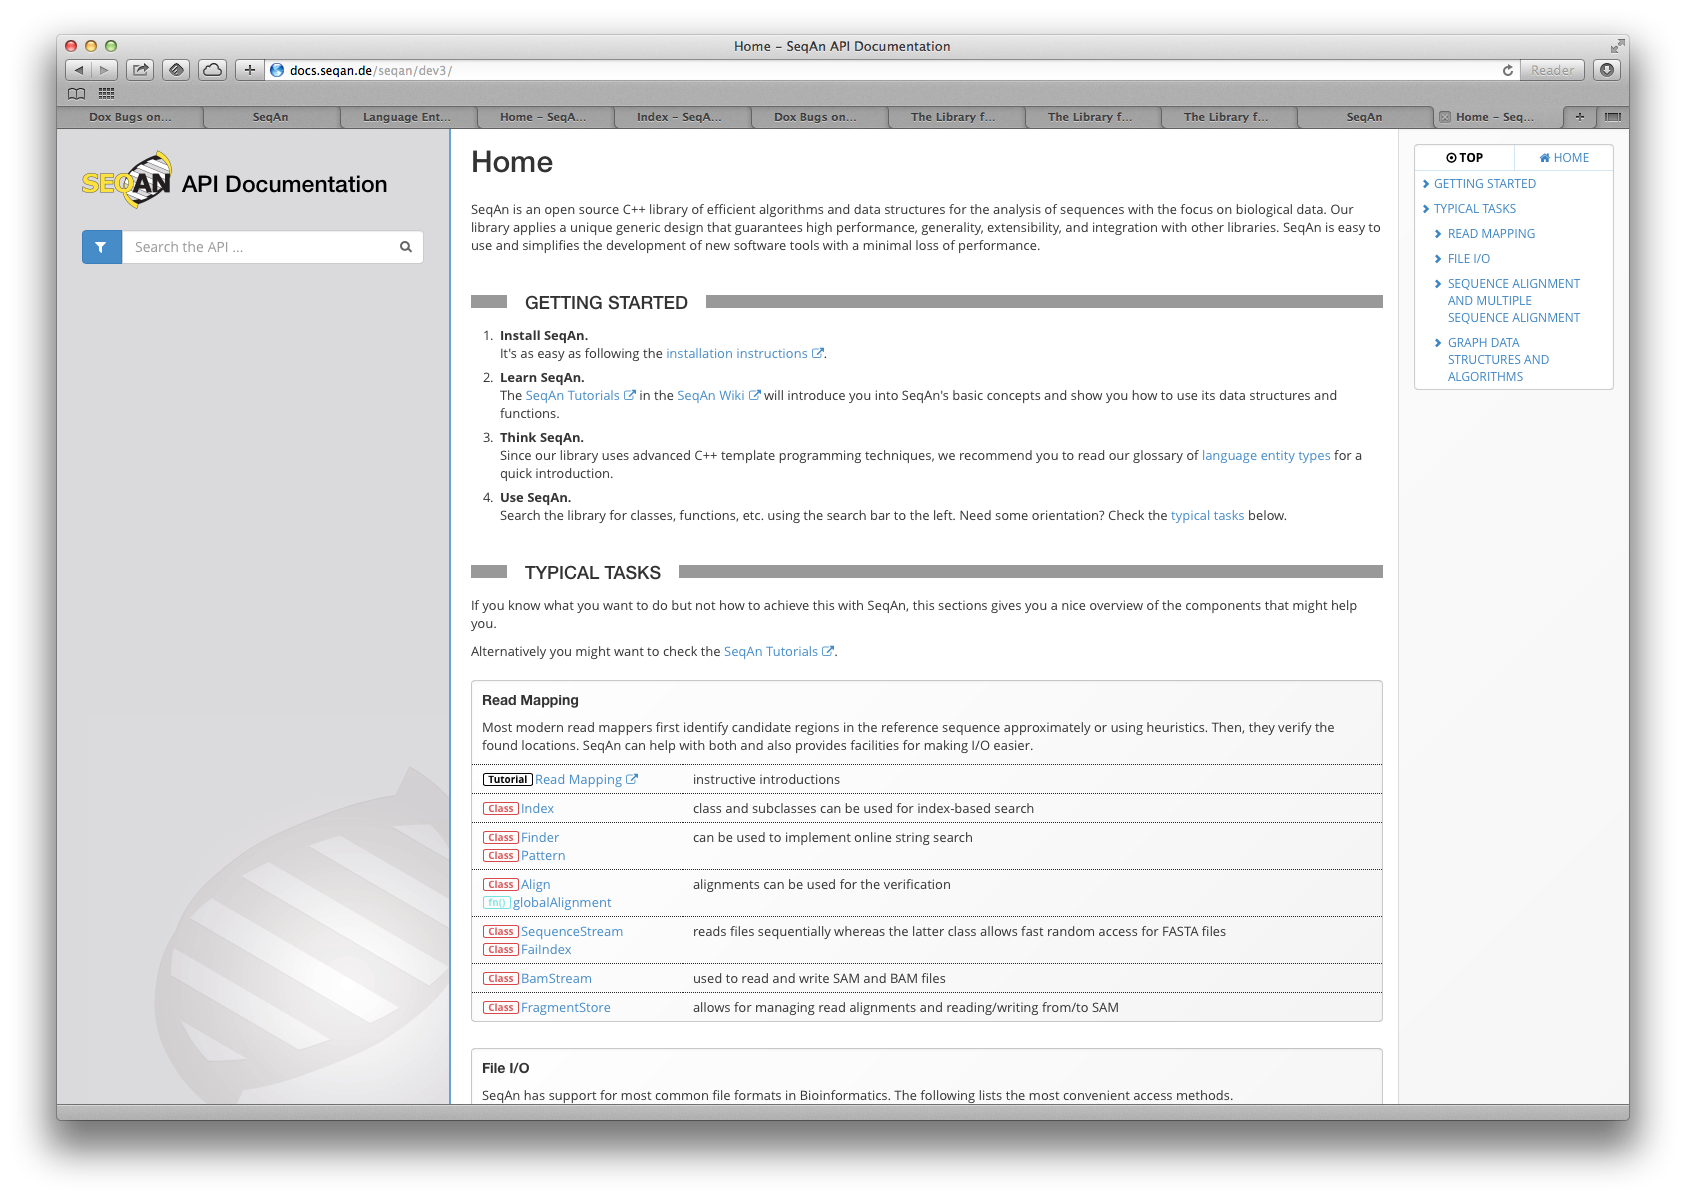
\includegraphics[width=\linewidth]{Figures/dox/dox-3_0_0-large-home.png}
                \caption{Startseite in Version 3.0.0}
                \label{fig:dox-large-home-3.0.0}
        \end{subfigure}%
        \vskip\baselineskip
        \begin{subfigure}[b]{0.38\linewidth}
                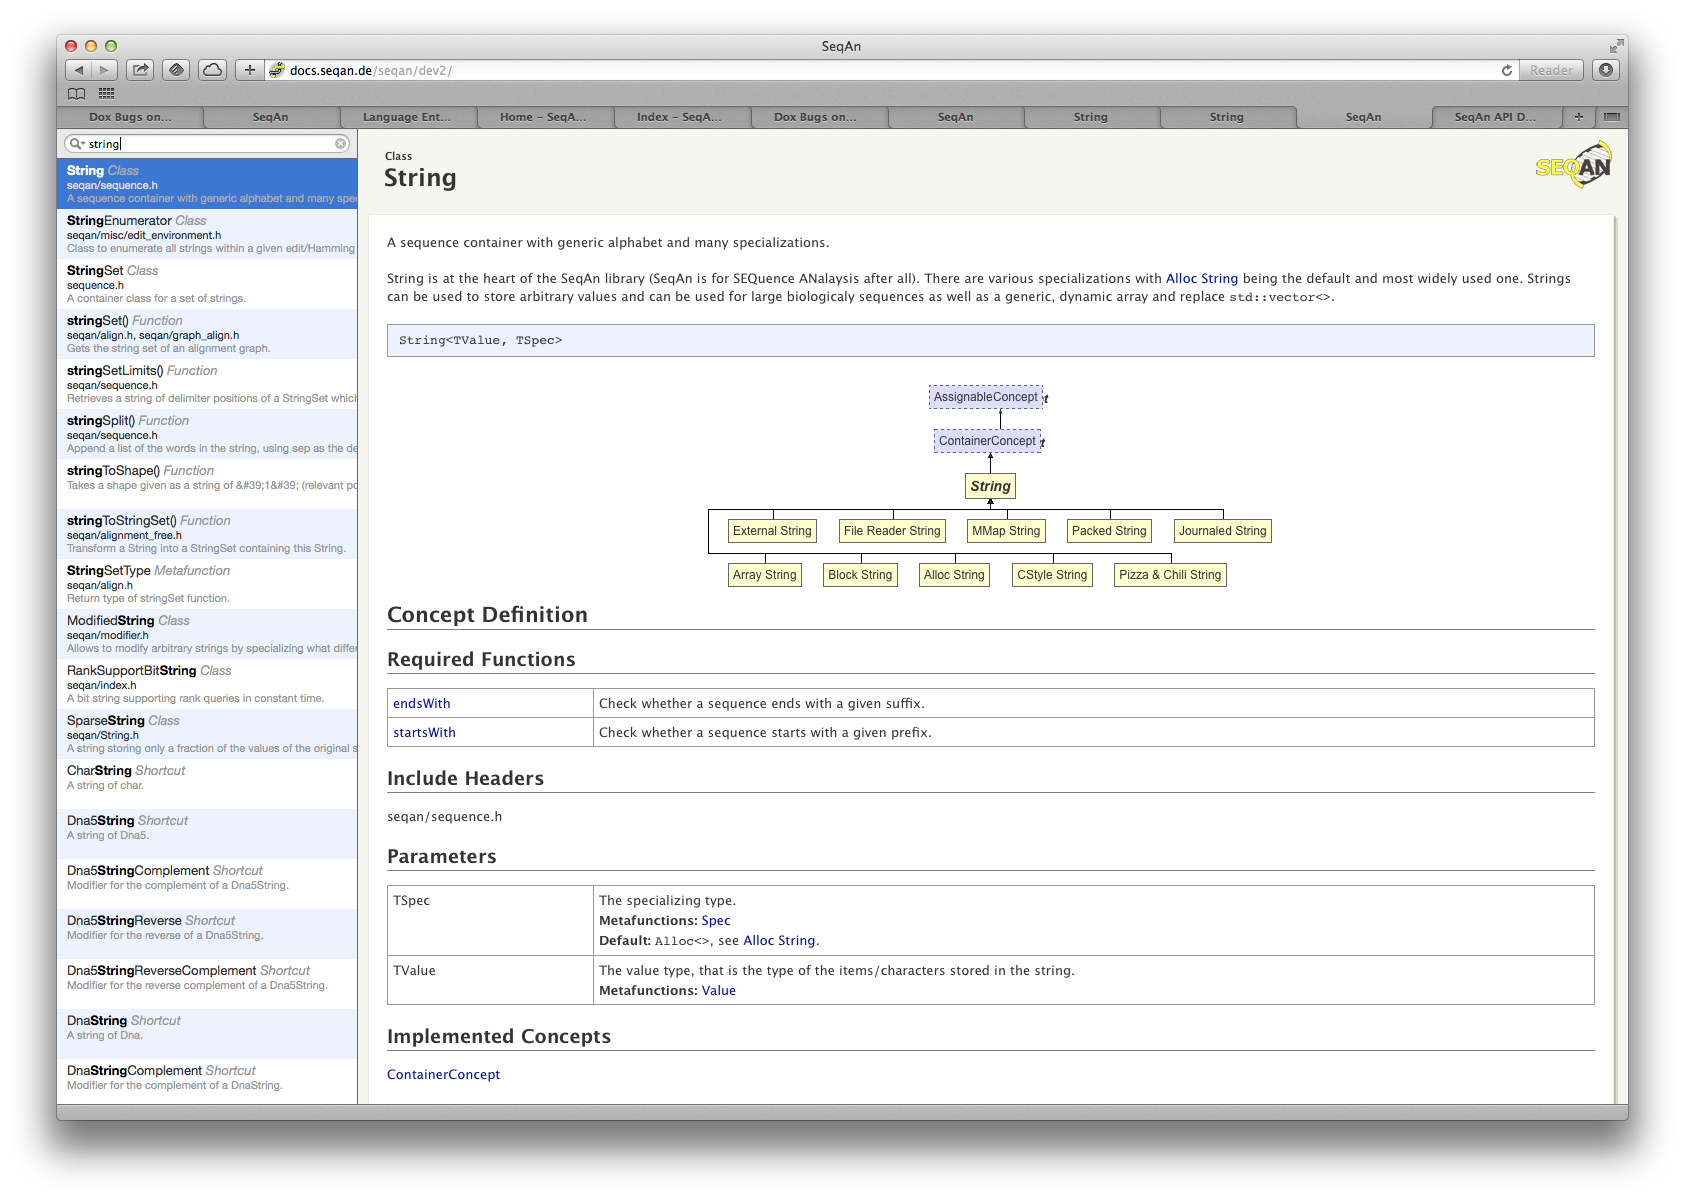
\includegraphics[width=\linewidth]{Figures/dox/dox-2_0_0-large-string-opened.png}
                \caption{Geöffnete \texttt{String}-Klasse in Version 2.0.0}
                \label{fig:dox-large-string-opened-2.0.0}
        \end{subfigure}
        \hspace{1cm}
        \begin{subfigure}[b]{0.38\linewidth}
                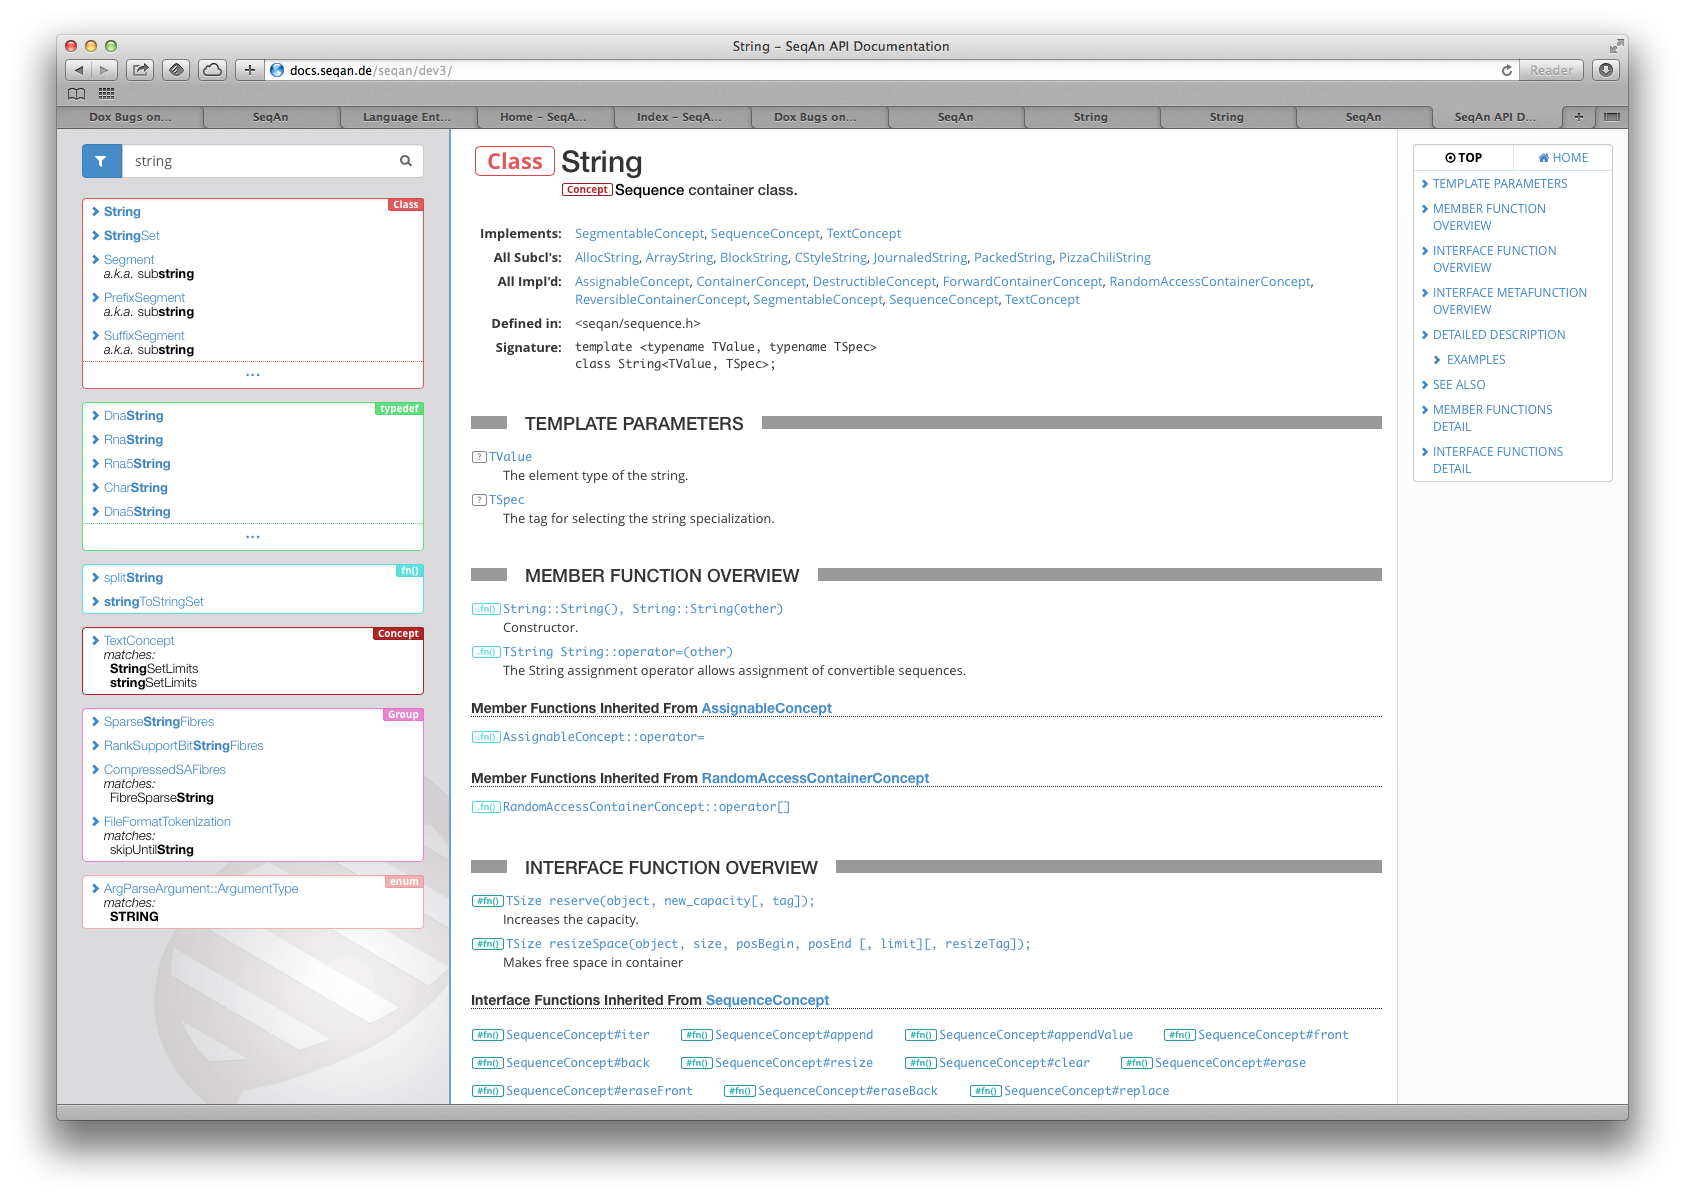
\includegraphics[width=\linewidth]{Figures/dox/dox-3_0_0-large-string-opened.png}
                \caption{Geöffnete \texttt{String}-Klasse in Version 3.0.0}
                \label{fig:dox-large-string-opened-3.0.0}
        \end{subfigure}
        \caption[Alte und neue Dokumentation im Vergleich --- in normaler Breite]{Die Abbildungen zeigen die alte und neue Dokumentation.}
        \label{fig:dox-large-all}
\end{figure}
\end{landscape}
\restoregeometry










\paragraph{Dokumentationssystem}

In Vorbereitung auf die technische Neuentwicklung der Dokumentation haben meine Kollegen und ich zunächst das in SeqAn verwendete Dokumentationssystem überarbeitet.

Der SeqAn-Entwickler Gogol Döring entwarf das \code[apiua://code/-9223372036854774817]{Dokumentationssystem} \textit{DDDoc} im Zuge einer \textit{expliziten-argumentativen} \code{apiua://code/-9223372036854775281}. Notwendig war (und ist) ein selbst entwickeltes Dokumentationssystem, da SeqAn, die noch nicht in den C\texttt{++}-Sprachstandard aufgenommene Sprachentität \textit{Concept} verwendet.\footnote{Gogol-Dörings Einschätzung, dass Concepts unbedingt Bestandteil der Dokumentation sein müssen, konnte ich empirisch bestätigen. Wie die Probleme \code{apiua://code/-9223372036854775280} und \code{apiua://code/-9223372036854775544} zeigen, können ohne Concepts die inhaltliche Zusammengehörigkeit technisch global implementierter \mbox{(Meta-)Funktionen} vom Anwender nicht erkannt werden. Tatsächlich handelt es sich nämlich bei den meisten globalen Funktionen inhaltlich um \mbox{Interface-(Meta-)Funktionen.}}

Wie das folgende kleine Beispiel zeigt, unterscheidet sich DDDoc von bekannten Dokumentationssystemen wie JavaDoc oder Doxygen, indem es ungewöhnlich zu lesen und zu schreiben ist.

\begin{center}
\begin{minted}[linenos=false, firstnumber=1]{cpp}
/**
.Spec.SimpleScore
..general:Class.Score
..summary:Basic scoring scheme.
..description:
This class allows to do alignments with simple match/mismatch-based scores.
..remarks:This class also supports different gap open and extension costs.
..include:seqan/score.h
*/
\end{minted}
\captionof{listing}{DDDoc-Beispiel für die Template-Spezialisierung \texttt{SimpleScore}}
\label{lst:dddoc}
\end{center}

\bigskip

Mit meinem Vorschlag, das Format zu überarbeiten, rannte ich bei den SeqAn-Entwicklern offene Türen ein. Eine Überarbeitung würde außerdem die Möglichkeit bieten, die in DDDoc fehlende Unterscheidung zwischen den Beziehungen ``wird von Funktion verwendet'' und ``ist Teil der Schnittstelle eines Typs'' zu beheben. Aus diesen Gründen wurde ein Doxygen-Derivat namens \textit{Dox} entwickelt, das auch Concepts und damit auch globale Funktionsinterfaces und Templatevererbung unterstützt. Implementiert wurde ebenso ein C{}\verb!++!-Parser.

Das folgende Beispiel zeigt denselben Dokumentationseintrag im neuen Dox-Format:

\begin{center}
\begin{minted}[linenos=false, firstnumber=1]{cpp}
/*!
 * @class SimpleScore
 * @extends Score
 * @summary Basic scoring scheme.
 *
 * @signature template <typename TValue>
 *            class Score<Tvalue, Simple>;
 *
 * This class allows to do alignments with simple match/mismatch-based 
 * scores.
 */
template <typename TValue>
class Score<TValue, Simple> {...};
\end{minted}
\captionof{listing}{Dox-Beispiel für die Template-Spezialisierung \texttt{SimpleScore}}
\label{lst:dox}
\end{center}

\bigskip

Wie man erkennen kann, ist das neue Doxygen-Format durch seine Ähnlichkeit zu JavaDoc und Doxygen leichter zu lesen und zu schreiben.

Das nächste und letzte Beispiel zeigt den Dokumentationseintrag für die technisch globale, aber inhaltlich zum \texttt{Score} gehörige Interface-Funktion \texttt{scoreGapOpen}:

\begin{center}
\begin{minted}[linenos, firstnumber=1]{cpp}
/*!
 * @fn Score#scoreGapOpen
 *
 * @signature TValue scoreGapOpen(sc);
 *
 * @return TValue The gap open score value for <tt>sc</tt>.
 *         Tvalue is the value type of <tt>sc</tt>.
 * @param sc The @link Score @endlink object to query.
 */
template <typename TValue, typename TSpec, typename TSeqHValue, typename TSeqVValue>
inline TValue
scoreGapOpen(...)
\end{minted}
\captionof{listing}{Dox-Beispiel für die zur Klasse \texttt{Score} gehörige Interface-Funktion \texttt{scoreGapOpen}}
\label{lst:dox2}
\end{center}

\bigskip

Über mehrere Monate haben die SeqAn-Entwickler sämtliche DDDoc-Einträge zu Dox-Einträgen umgewandelt. Beim Debuggen dieser Umwandlungen half u.a. ein in der neuen Dokumentation implementierter Entwicklermodus.



\paragraph{Entwicklermodus}

Für die neue Dokumentation habe ich einen Entwicklermodus entwickelt, der sich an die SeqAn-Entwickler richtet. Der Entwicklermodus kann bei geöffneter Dokumentation durch die Tastenkombination \texttt{Shift+Ctrl}\footnote{Zu beachten ist, dass der rechte Bereich, also nicht der Suchbereich, über den Fokus verfügen muss.} aktiviert werden und wurde von mir so implementiert, dass er um beliebige Funktionen erweitert werden kann. Aktuell unterstützt er SeqAn-Entwickler bei den folgenden Tätigkeiten:
\begin{itemize}
  \item SeqAn-Entwickler können für jeden Dokumentationseintrag den dazugehörigen Dox-Eintrag im Quellcode einblenden lassen (siehe \fref{fig:dox-devmode-dox}).
  \item Insbesondere für das Schreiben von Tutorials benötigen SeqAn-Entwickler den Link zu einem bestimmten Eintrag. Dieser kann nicht ohne Weiteres aus der Adresszeile entnommen werden. Einerseits verwendet die Dokumentation \textit{IFrames}\footnote{\url{https://www.w3.org/wiki/HTML/Elements/iframe}}. Andererseits gibt es den Bedarf, auch einen ganz bestimmten Untereintrag innerhalb eines Dokumentationseintrages zu verlinken. Im Entwicklermodus werden alle verlinkbaren Elemente hervorgehoben. Ein Klick auf eines dieser Elemente bringt einen modalen Dialog hervor, der alle Verlinkungsmöglichkeiten anzeigt und auf Wunsch in die Zwischenablage kopiert (siehe \fref{fig:dox-devmode-permalink}).
\end{itemize}

Der Entwicklermodus wurde von den SeqAn-Entwicklern sehr gut angenommen, was man leicht an den schnellen Beschwerden, im Falle von entdeckten Bugs, sehen konnte.

\begin{figure}[ht!]
  \centering
    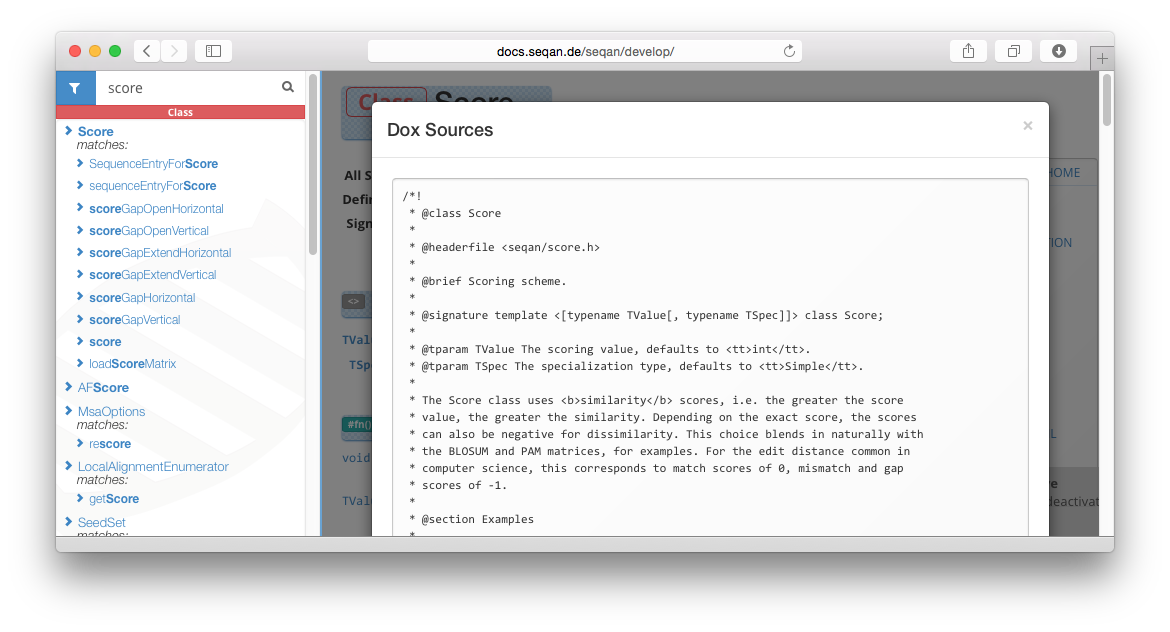
\includegraphics[width=0.9\linewidth]{Figures/dox/devmode-dox.png}
    \caption{Entwicklermodus --- Dox-Quelle für den aktuellen Dokumentationseintrag}
    \label{fig:dox-devmode-dox}
\end{figure}

\begin{figure}[ht!]
  \centering
    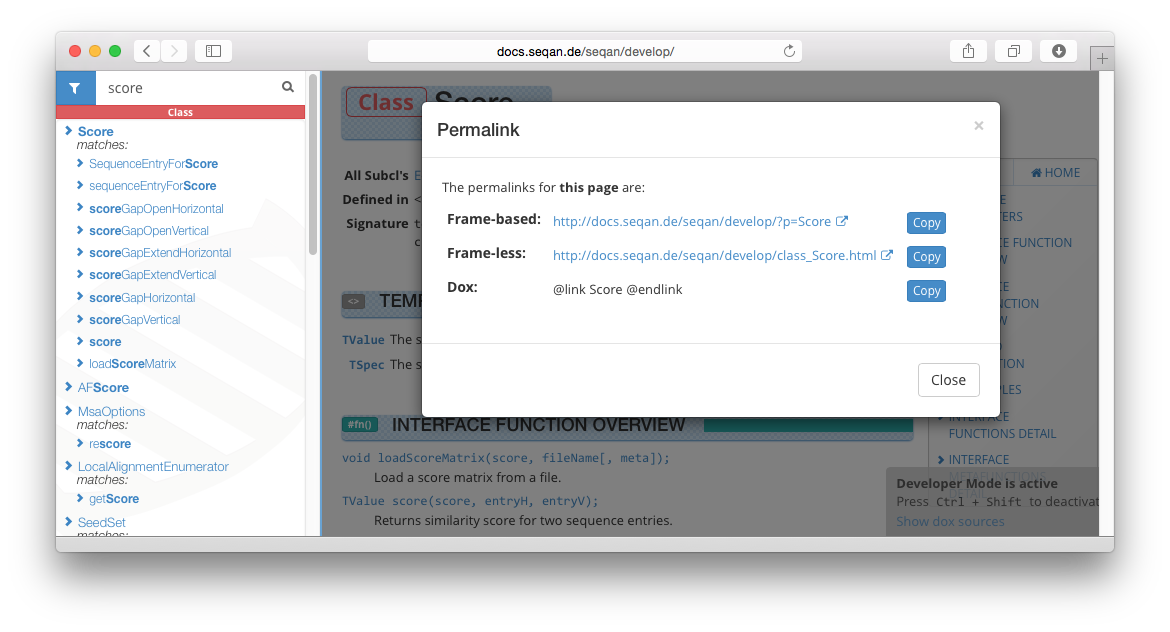
\includegraphics[width=0.9\linewidth]{Figures/dox/devmode-permalink.png}
    \caption[Entwicklermodus --- Anzeige aller Links für das aktuell selektierte Element]{Entwicklermodus: Anzeige aller Links für das aktuell selektierte Element. Im Hintergrund des modalen Dialogs kann man drei bläulich hinterlegte Elemente erkennen, die verlinkbar sind.}
    \label{fig:dox-devmode-permalink}
\end{figure}

%API-Entwickler müssen gute Dokumentation schreiben \citep{Kramer:1999ih}



\paragraph{Gesamtüberblick}

Die Notwendigkeit eines Gesamtüberblicks konnte ich empirisch zeigen und lässt sich auch direkt und indirekt aus der Literatur entnehmen. So verhindert ein fehlender Gesamtüberblick Top-Down-Lernen \citep[vgl.][]{Brooks:1983fj} und das Erkennen von Zusammengehörigkeit verteilter Informationen \citep[vgl.][]{BenShneiderman:gn} --- insbesondere für Anfänger \citep{Stylos:2008jt,Piccioni:2013uq}.

Werden an keiner Stelle Entwurfsentscheidungen gebündelt dargestellt, werden Anwender beim Anpassungen von Beispiel-Code eingeschränkt \citep{Bruch:2006bv}. Dies führt dazu, dass Anwender häufiger Fehler bei der Anpassung machen, und mit geringerer Wahrscheinlichkeit die korrekte Intention des Codes wiedergeben \citep{Fairbanks:2006jw}.

Außerdem muss die Startseite der Dokumentation über eine Aufgaben-bezogene, logische Gruppierung der Library-Elemente verfügen, da es klassenübergreifende Aufgaben gibt, deren Lösung sich für API-Anfänger sonst nicht ohne Weiteres erschließen würde. \citep{DaqingHou:2005ba,clarke:2006}

Die überarbeitete Startseite der SeqAn-Dokumentation verfügt nun über folgende Elemente:
\begin{itemize}\itemsep1pt\parskip0pt\parsep0pt
  \item Knappe Beschreibung von SeqAn
  \item \textit{Getting Started}
  \begin{itemize}
    \item Verweis auf die Installationsanleitungen
    \item Verweise auf die Tutorials und ähnliche Inhalte (Profiling, CMake, etc.)
    \item Verweis auf die Sprachentitätstypen-Übersichtseite
  \end{itemize}
  \item Typische SeqAn-Aufgaben mit Verweisungen auf die dazugehörigen Tutorials, Klassen und Funktionen. Die vier typischen Aufgaben lauten:
  \begin{itemize}
    \item Read-Mapping
    \item Ein- u. Ausgabe
    \item Sequence-Alignment
    \item Graphen
  \end{itemize}
\end{itemize}

Des Weiteren wurde das kaum auffindbare und veraltete Background-and-Motivation-Tutorial\footnote{\url{http://seqan.readthedocs.org/en/master/Tutorial/BackgroundAndMotivation.html}} umfassend überarbeitet. Es erklärt nun die Motivation der SeqAn zu Grunde liegenden Entwurfsentscheidungen und veranschaulicht den SeqAn-Performance-Gewinn an Hand eines ohne SeqAn geschriebenen Beispiels.

%High-level Design-Dokumentation notwendig \citep{Robillard:2009cs}
%Globale Designentscheidungen müssen auf Startseite der Doku erklärt werden \citep{Robillard:2009cs}




\paragraph{Sprachentitätstypen}

Das Konzept der \code{apiua://code/-9223372036854775413} (engl. \textit{language entity types}) ist in SeqAn von besonders großer Relevanz, da SeqAn durch den Gebrauch von Concepts Sprachentitätstypen verwendet, die dem Gros der SeqAn-Anwender unbekannt sind (siehe \sref{sec:gt-let}). Dabei ist es von elementarer Wichtigkeit, bedeutende Konzepte in einer Dokumentation zu erklären \citep{Jeong:kf,Ko:2011vw,Monperrus:2011bf}.

Mein Ziel war es, Anwender unaufdringlich auf die Existenz neuer Sprachentitätstypen hinzuweisen und es ihnen zu erlauben, sich auf leichtgewichtige Art darüber zu informieren. Dieser Ansatz wird als \textit{knowledge pushing} bezeichnet und wurde bereits in ähnlicher Weise von \cite{Watson:2009da,sunshine2014searching} erfolgreich angewendet.

Die Umsetzung erfolgte wie folgt:
\begin{itemize}
  \item Alle in der Dokumentation genannten Sprachentitäten, wie \texttt{length} oder \texttt{String}, werden durch ein kleines Label annotiert.
  \item Jedes Label kennzeichnet einen Sprachentitätstyp.
  \item Die Labels werden durch zwei Merkmale unterschieden:
  \begin{enumerate}
    \item Farbe, welche die Zusammengehörigkeit verschiedener Sprachentitätstypen symbolisiert.
    \item Ideogramm, also ein textuelles Piktogramm, das den Sprachentitätstyp phänotypisch ausdrückt.
  \end{enumerate}
  \item Die existierenden Sprachentitätstypen lauten:
  \begin{itemize}
    \item[] \raisebox{-0.4ex}{
\includegraphics[height=1em]{Figures/lets/typedef.png}} Typdefinition mittels \texttt{typedef}
    \hspace{1em} \raisebox{-0.4ex}{
\includegraphics[height=1em]{Figures/lets/variable.png}} Variable\footnote{Beim Schreiben dieser Dissertation wurde mir klar, dass \textit{var} ein geeigneteres Ideogramm darstellt. Ein entsprechender Issue-Tracker-Eintrag existiert: \url{https://github.com/seqan/seqan/issues/1034}}
    
    \item[] \raisebox{-0.4ex}{
\includegraphics[height=1em]{Figures/lets/concept.png}} Concept
    \hspace{1em} \raisebox{-0.4ex}{
\includegraphics[height=1em]{Figures/lets/class.png}} Klasse
    \hspace{1em} \raisebox{-0.4ex}{
\includegraphics[height=1em]{Figures/lets/spec.png}} Spezialisierung
    \hspace{1em} \raisebox{-0.4ex}{
\includegraphics[height=1em]{Figures/lets/enum.png}} Enum
    
    \item[] \raisebox{-0.4ex}{
\includegraphics[height=1em]{Figures/lets/globalmetafunction.png}} Globale Metafunktion
    \hspace{1em} \raisebox{-0.4ex}{
\includegraphics[height=1em]{Figures/lets/interfacemetafunction.png}} Interface-Metafunktion
    \hspace{1em} \raisebox{-0.4ex}{
\includegraphics[height=1em]{Figures/lets/tag.png}} Tag
    
    \item[] \raisebox{-0.4ex}{
\includegraphics[height=1em]{Figures/lets/globalfunction.png}} Globale Funktion
    \hspace{1em} \raisebox{-0.4ex}{
\includegraphics[height=1em]{Figures/lets/interfacefunction.png}} Interface-Funktion
    \hspace{1em} \raisebox{-0.4ex}{
\includegraphics[height=1em]{Figures/lets/memberfunction.png}} Member-Funktion

    \item[] \raisebox{-0.4ex}{
\includegraphics[height=1em]{Figures/lets/adaption.png}} Adaption
    \hspace{1em} \raisebox{-0.4ex}{
\includegraphics[height=1em]{Figures/lets/makro.png}} Makro
  \end{itemize}
  \item Bewegt der Anwender die Maus über ein Label, wird eine minimale Beschreibung des dazugehörigen Sprachentitättyps eingeblendet (siehe \fref{fig:dox-let-hover}).
  \item Klickt der Anwender bei eingeblendeter minimaler Beschreibung auf das Label, wird die ausführlichere Beschreibung des Sprachentitättyps geöffnet (siehe \fref{fig:dox-let-detail}).
  \item Sowohl Suchergebnisse als auch Funktionsauflistungen innerhalb von Dokumentationseinträgen sind nach den Sprachentitätstypen gruppiert (siehe \fref{fig:dox-large-string-opened-3.0.0}).
  \item Die Suchfunktion der Dokumentation erlaubt die Filterung der Ergebnisse nach Sprachentitätstypen. Tatsächlich ging es mir aber nicht um die Funktion selbst, sondern darum, dass neugierige Anwender so auf eine vollständige Auflistung der in SeqAn präsenten Sprachentitätstypen stoßen, ohne sich mit diesen gleich aktiv auseinandersetzen zu müssen.
\end{itemize}

\begin{figure}[ht!]
  \centering
    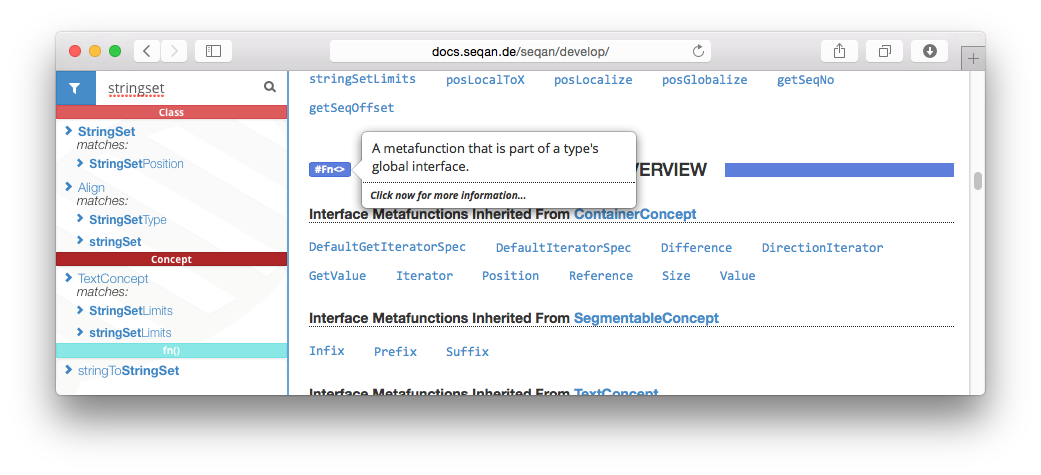
\includegraphics[width=0.9\linewidth]{Figures/dox/let-hover.png}
    \caption{Kurzbeschreibung des Sprachentitättyps \textit{Interface-Metafunktion}}
    \label{fig:dox-let-hover}
\end{figure}

\begin{figure}[ht!]
  \centering
    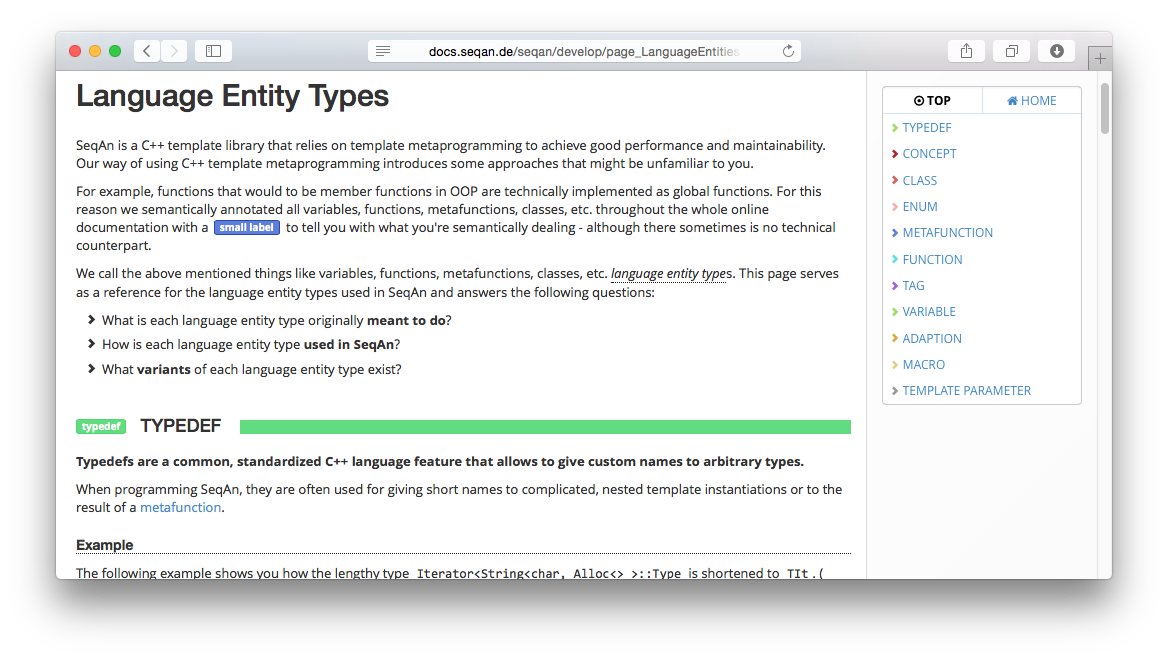
\includegraphics[width=0.9\linewidth]{Figures/dox/let-detail.png}
    \caption{Ausführliche Beschreibung der in SeqAn verwendeten Sprachentitätstypen}
    \label{fig:dox-let-detail}
\end{figure}



\paragraph{Seitenaufbau}

Der Aufbau von Dokumentationsseiten wurde von mir und einem SeqAn-Entwickler überarbeitet. Abstrakt sind Seiten wie folgt gegliedert:
\begin{enumerate}
\itemsep1pt\parskip0pt\parsep0pt
  \item Zusammenfassung zum Nachschlagen
  \item Detaillierte Beschreibung
\end{enumerate}

Im Grunde gibt es zwei Seitentypen:
\begin{description}
  \item[Containerseiten] kommen zur Dokumentation von Concepts, Klassen und Spezialisierungen zum Einsatz\footnote{Beispiel String-Klasse: \url{http://docs.seqan.de/seqan/develop/?p=String}}, da diese Sprachentitätstypen über Untereinträge verfügen. Hierbei umfasst die Zusammenfassung einen Bereich für Metainformationen und eine Auflistung aller verfügbaren Funktionen. Die Metainformationen zählen bei Klassen beispielsweise auf, welche Concepts direkt und indirekt implementiert werden, welche Spezialisierungen existieren, in welcher Datei die Klasse definiert ist und welche Signatur die Klasse besitzt. Die Auflistung der Funktionen ist gegliedert nach Member-Funktionen, Interface-Funktionen und Interface-Metafunktionen. Der Detailbereich erläutert im Falle einer Klasse den Gebrauch der Klasse samt Beispielen und erklärt detailliert sämtliche oben genannten Funktionen im Detail.
  \item[Elementseiten] sind atomar und kommen für alle anderen Sprachentitätstypen zum Einsatz\footnote{Beispiel globalAlignment-Funktion: \url{http://docs.seqan.de/seqan/develop/?p=globalAlignment}}, da diese über keine Untereinträge verfügen. Im Falle von (semantisch) globalen Funktionen umfasst die Zusammenfassung eine Auflistung aller Parameter und die Beschreibung der Rückgaben. Der Detailbereich erläutert dann wiederum ausführlich Sinn und Zweck der Funktion und beschreibt dies an Hand von Beispielen.
\end{description}

In SeqAn werden häufig Referenzen technisch als Eingaben übergeben, inhaltlich aber als Rückgaben behandelt. Ob ein Parameter als Ein- und/oder Ausgabe behandelt wird, wird durch die folgenden Icons ausgezeichnet: 
\includegraphics[height=.7em]{Figures/dox/in.png}, 
\includegraphics[height=.7em]{Figures/dox/out.png} und 
\includegraphics[height=.7em]{Figures/dox/inout.png}.


\paragraph{Beispiele}

Beispiele sind neben der Gesamtübersicht der wichtigste Bestandteil einer benutzerfreundlichen Dokumentation \citep{Robillard:2010bh}, was ich an Hand der verschiedenen, durch die Abwesenheit (guter) Beispiele eingeschränkten Beispiel-bezogenen Strategien empirisch belegen konnte (siehe \sref{sec:dox}).

Im Zuge der inhaltlichen Überarbeitung der Dokumentation wurden für die wichtigsten Dokumentationseinträge existierende Beispiele verbessert und fehlende Beispiele ergänzt. Dabei wurden alle Beispiele um die Programmausgabe ergänzt, was besonders für API-Endanwender wichtig ist \citep{Gross:2010iz}.



\paragraph{Suchfunktion}

Die vollständig neu entwickelte Suchfunktion verfügt über die folgenden Funktionen:
\begin{itemize}
  \item Sprachentitäten können nun über Aliasse/Synonyme verfügen. Auf diese Weise wurden die im \textit{Vocabulary Problem} \citep{Furnas:1987hl} veranlagten Usability-Probleme gemildert. Der Suchbegriff \texttt{substring} beispielweise führt nun auch zu dem Treffer \textit{infix}. Wurde ein Eintrag mit Hilfe eines Synonyms gefunden, wird dem Anwender dies mitgeteilt. Auf diese Weise lernt der Anwender bedarfsgerecht die korrekte Bezeichnung in SeqAn. Anwender, die ohnehin den korrekten Begriff verwendet haben, erfahren nicht von den Synonymen. Auf diese Weise wird verhindert, dass unterschiedlich benannte, aber inhaltlich identische Sprachentitäten innerhalb von SeqAn gepflegt werden müssen.
  \item Die Suchergebnisse sind nun gewichtet, so dass beispielsweise der Suchbegriff \texttt{string} auch tatsächlich die \texttt{String}-Klasse als ersten Suchtreffer hervorbringt.
  \item Die Suchergebnisse sind nach Sprachentitätstypen gruppiert und auf maximal fünf Einträge je Typ begrenzt. Auslassungspunkte am Ende einer Treffergruppe deuten darauf hin. Ein Klick darauf zeigt alle Suchtreffer der Gruppe.
  \item Suchergebnisse können auch Dokumentationsteileinträge sein. So ist der erste Suchtreffer für \texttt{infix}, die \texttt{Infix}-Interface-Metafunktion innerhalb des Concepts \texttt{SegmentableConcept}. Der Anwender kann selbst wählen, ob der den Dokumentationseintrag oder -untereintrag öffnen möchte.
  \item Die Suche kann ohne Maus und ausschließlich mit der Tastatur bedient werden. Dazu erhält das Suchfeld automatisch den Fokus, die Sucheingabe kann mit \texttt{Esc} gelöscht und innerhalb der Suchergebnisse mit den Pfeiltasten navigiert werden.
\end{itemize}

  



\paragraph{Darstellung}

Die Online-Dokumentation ist \textit{responsive}\footnote{\url{https://developers.google.com/web/fundamentals/layouts/rwd-fundamentals/}}, passt sich also einer großen Bandbreite von Fenstergrößen an. Dies ist nicht nur schick, sondern auch hilfreich. Bei SeqAn-Anfängern konnte ich einen häufigen Wechsel zwischen Entwicklungsumgebung und Online-Dokumentation beobachten. Da die neue SeqAn-Dokumentation selbst bei einem 600 Pixel schmalen Fenster (bei 72 DPI) ohne Einschränkung nutzbar ist, können SeqAn-Anwender die Dokumentation auch neben der Entwicklungsumgebung platzieren. Auch ist eine Nutzung der Dokumentation auf mobilen Geräten möglich, wie es einige Anwender forderten.

Des Weiteren habe ich großen Wert auf eine hohe Ästhetik gelegt. Ich denke, dieses u.a. durch den Einsatz von subtilen Farbverläufen und dezenten Animationen erreicht zu haben. Spaß an der Bedienung ist ein wesentlicher Aspekt des Anwendererlebnisses und spielt damit auch für SeqAns kommerziellen Erfolg eine Rolle.

\fref{fig:dox-small-all} stellt die gleichen Inhalte wie \fref{fig:dox-large-all} auf Seite \pageref{fig:dox-large-all} dar --- nur mit dem Unterschied eines schmaleren Browser-Fensters.

\newgeometry{inner=2cm,outer=1cm,top=1.5cm,bottom=1.5cm}
\thispagestyle{empty}
%\begin{landscape}
\begin{figure}
        \centering
        \begin{subfigure}[b]{0.48\linewidth}
                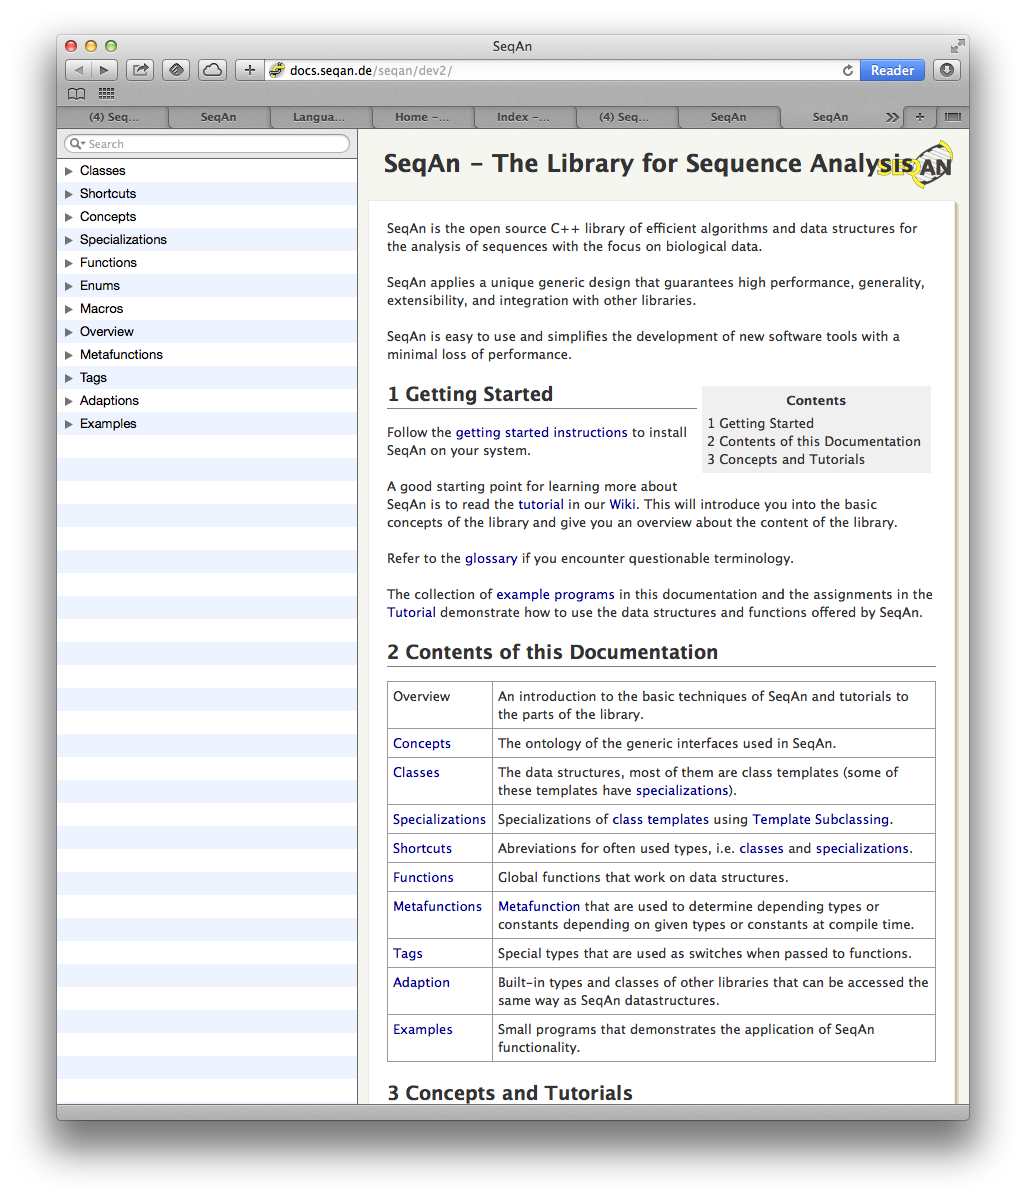
\includegraphics[width=\linewidth]{Figures/dox/dox-2_0_0-small-home.png}
                \caption{Startseite in Version 2.0.0}
                \label{fig:dox-small-home-2.0.0}
        \end{subfigure}
        \hfill
        \begin{subfigure}[b]{0.48\linewidth}
                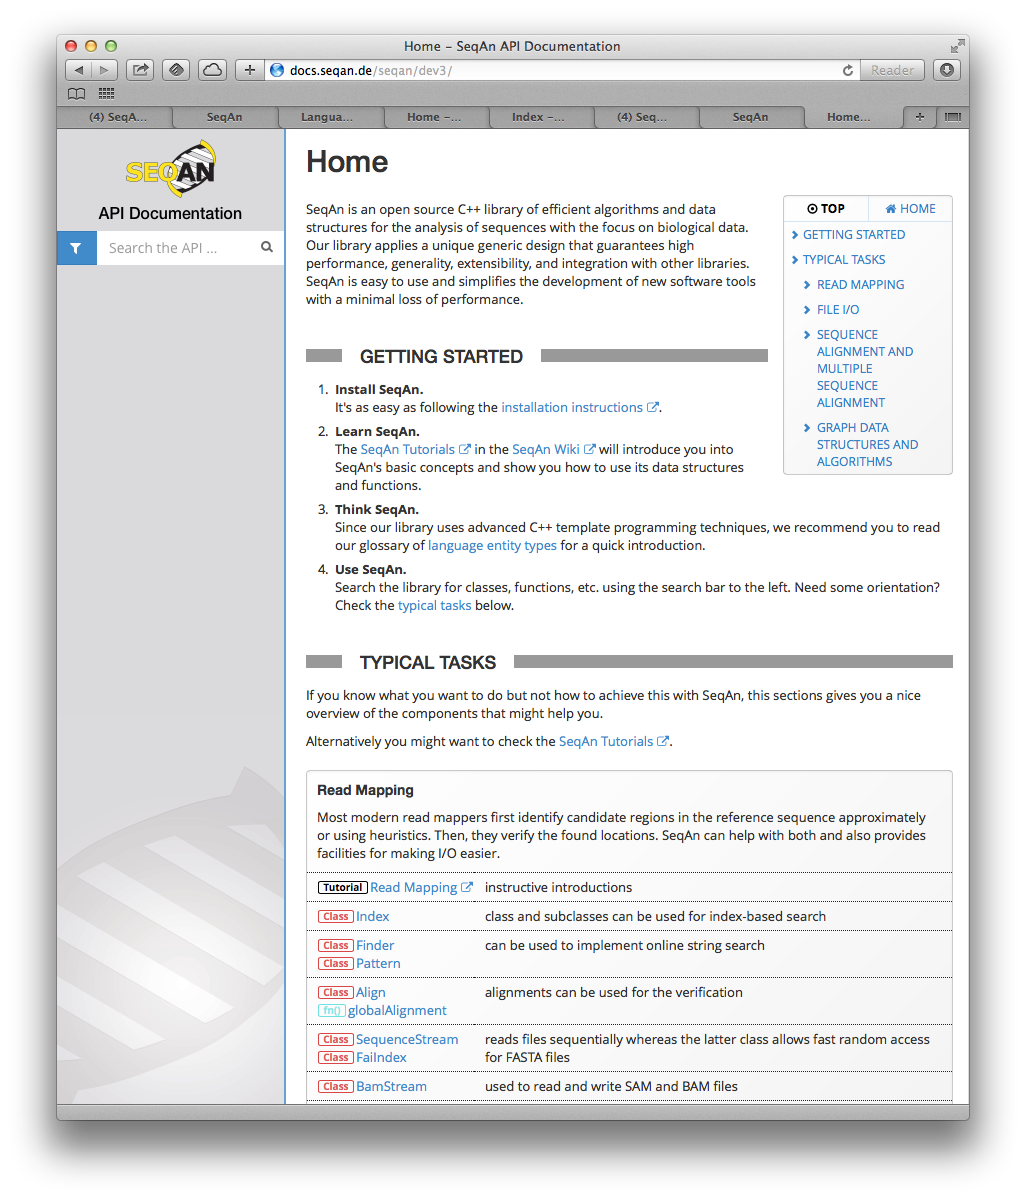
\includegraphics[width=\linewidth]{Figures/dox/dox-3_0_0-small-home.png}
                \caption{Startseite in Version 3.0.0}
                \label{fig:dox-small-home-3.0.0}
        \end{subfigure}%
        \vskip\baselineskip
        \begin{subfigure}[b]{0.48\linewidth}
                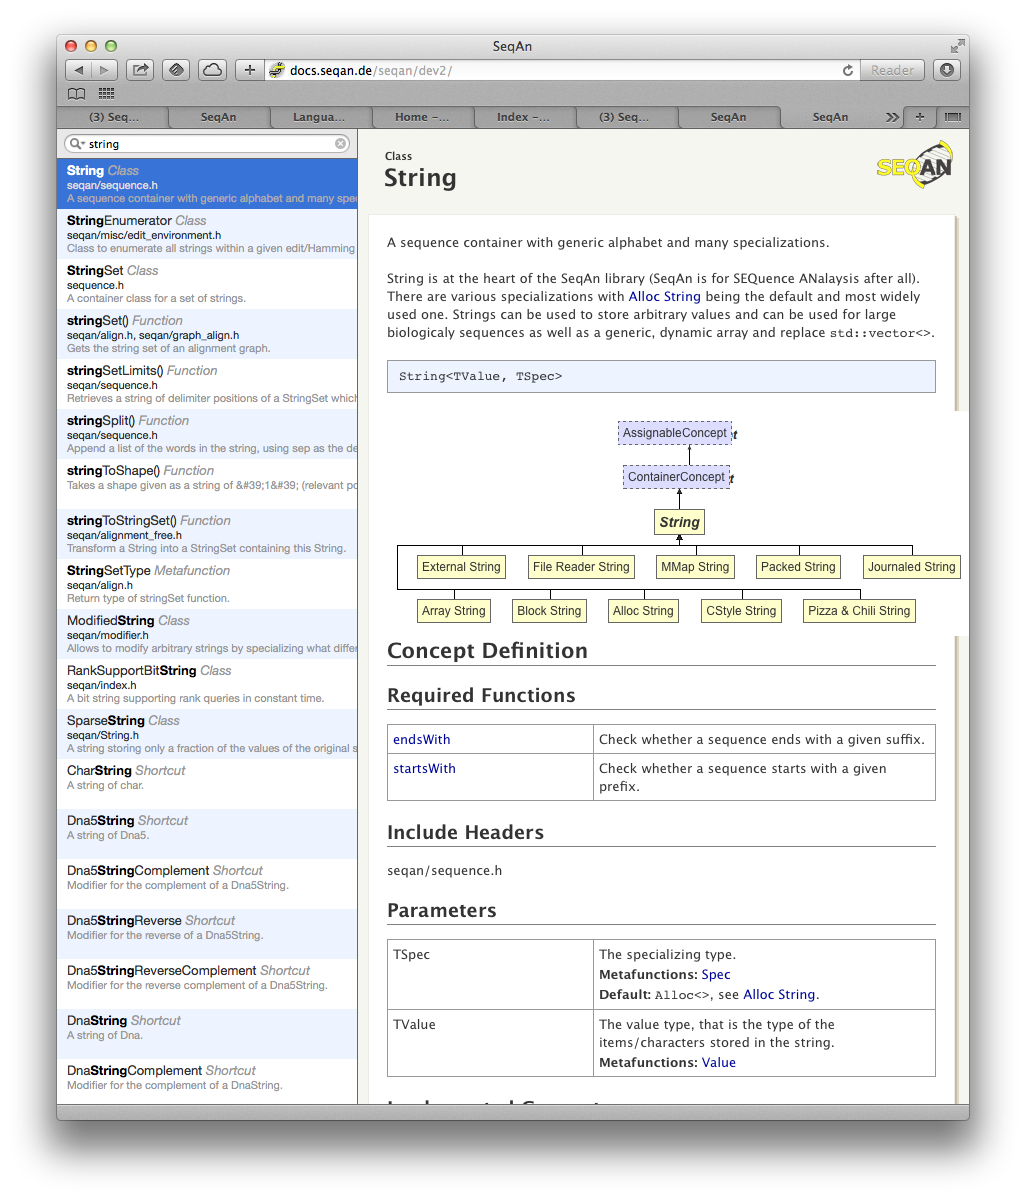
\includegraphics[width=\linewidth]{Figures/dox/dox-2_0_0-small-string-opened.png}
                \caption{Geöffnete \texttt{String}-Klasse in Version 2.0.0}
                \label{fig:dox-small-string-opened-2.0.0}
        \end{subfigure}
        \hfill
        \begin{subfigure}[b]{0.48\linewidth}
                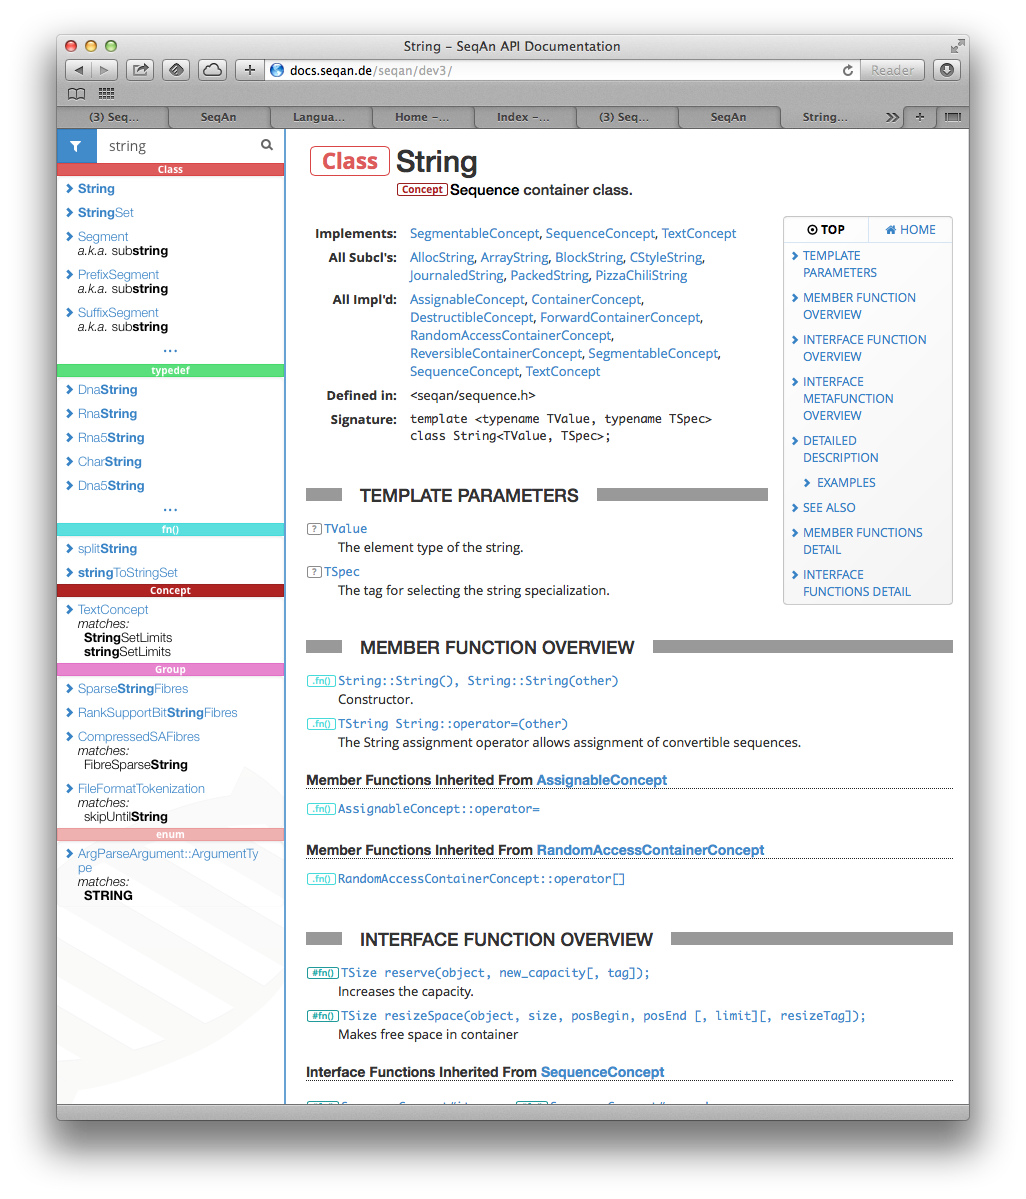
\includegraphics[width=\linewidth]{Figures/dox/dox-3_0_0-small-string-opened.png}
                \caption{Geöffnete \texttt{String}-Klasse in Version 3.0.0}
                \label{fig:dox-small-string-opened-3.0.0}
        \end{subfigure}
        \caption[Alte und neue Dokumentation im Vergleich --- in smaler Breite]{Die Abbildungen zeigen die alte und neue Dokumentation in schmaler Breite.}
        \label{fig:dox-small-all}
\end{figure}
%\end{landscape}
\restoregeometry




\paragraph{Integration}

Die neue Dokumentation ist besser in anderen Lernressourcen, wie den Tutorials, integriert. Dies wurde nicht zuletzt durch den weiter oben beschrieben Entwicklermodus gefördert, der SeqAn-Entwicklern alle möglichen Links für einen Dokumentations-(teil-)eintrag bereitstellt.  

Außerdem habe ich bei der Neuentwicklung auf die Indexierbarkeit durch Suchmaschinen geachtet. Dazu habe ich das Programm, welches die Dokumentation generiert, so angepasst, dass Inhalte sowohl statisch (für Suchmaschinen), als auch dynamisch (für Anwender) vorliegen.

Des Weiteren erfordert die Dokumentation --- trotz seines Funktionszuwachses --- keine Server-Komponente. Die mit SeqAn heruntergeladene Dokumentation verfügt online wie offline über den gleichen Funktionsumfang.







\begin{comment}
\newlength{\doxlargewidth}
\setlength{\doxlargewidth}{\linewidth}

\newlength{\doxnarrowwidth}
\setlength{\doxnarrowwidth}{0.61\doxlargewidth}

Donec urna leo, vulputate vitae porta eu, vehicula blandit libero. Phasellus eget massa et leo condimentum mollis. Nullam molestie, justo at pellentesque vulputate, sapien velit ornare diam, nec gravida lacus augue non diam. Integer mattis lacus id libero ultrices sit amet mollis neque molestie. Integer ut leo eget mi volutpat congue. Vivamus sodales, turpis id venenatis placerat, tellus purus adipiscing magna, eu aliquam nibh dolor id nibh. Pellentesque habitant morbi tristique senectus et netus et malesuada fames ac turpis egestas. Sed cursus convallis quam nec vehicula. Sed vulputate neque eget odio fringilla ac sodales urna feugiat.

\begin{figure}
  \centering
    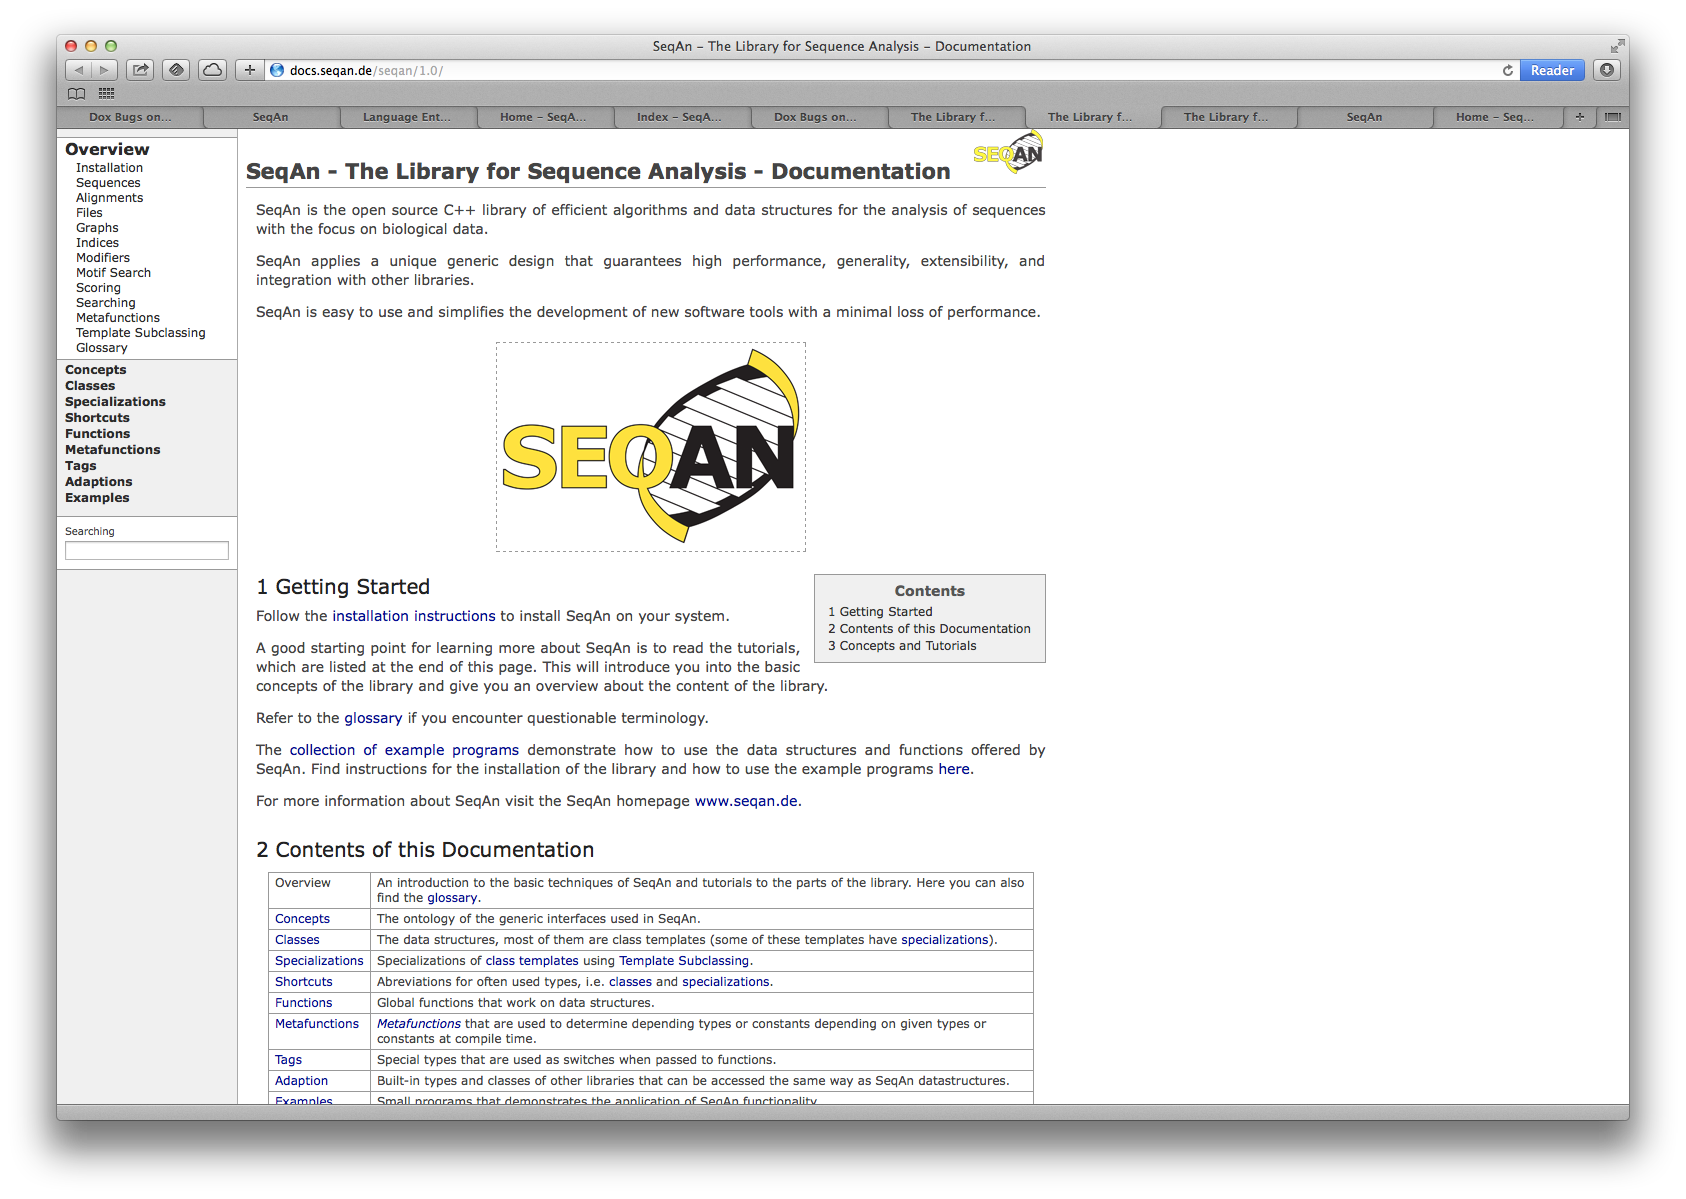
\includegraphics[width=\doxlargewidth]{Figures/dox/dox-1_0_0-large-home.png}
    \caption{Seqan-Online-Dokumentation in Version 1.0 - Breite Ansicht - Startseite}
    \label{fig:dox-1_0_0-large-home}
\end{figure}

\begin{figure}
  \centering
    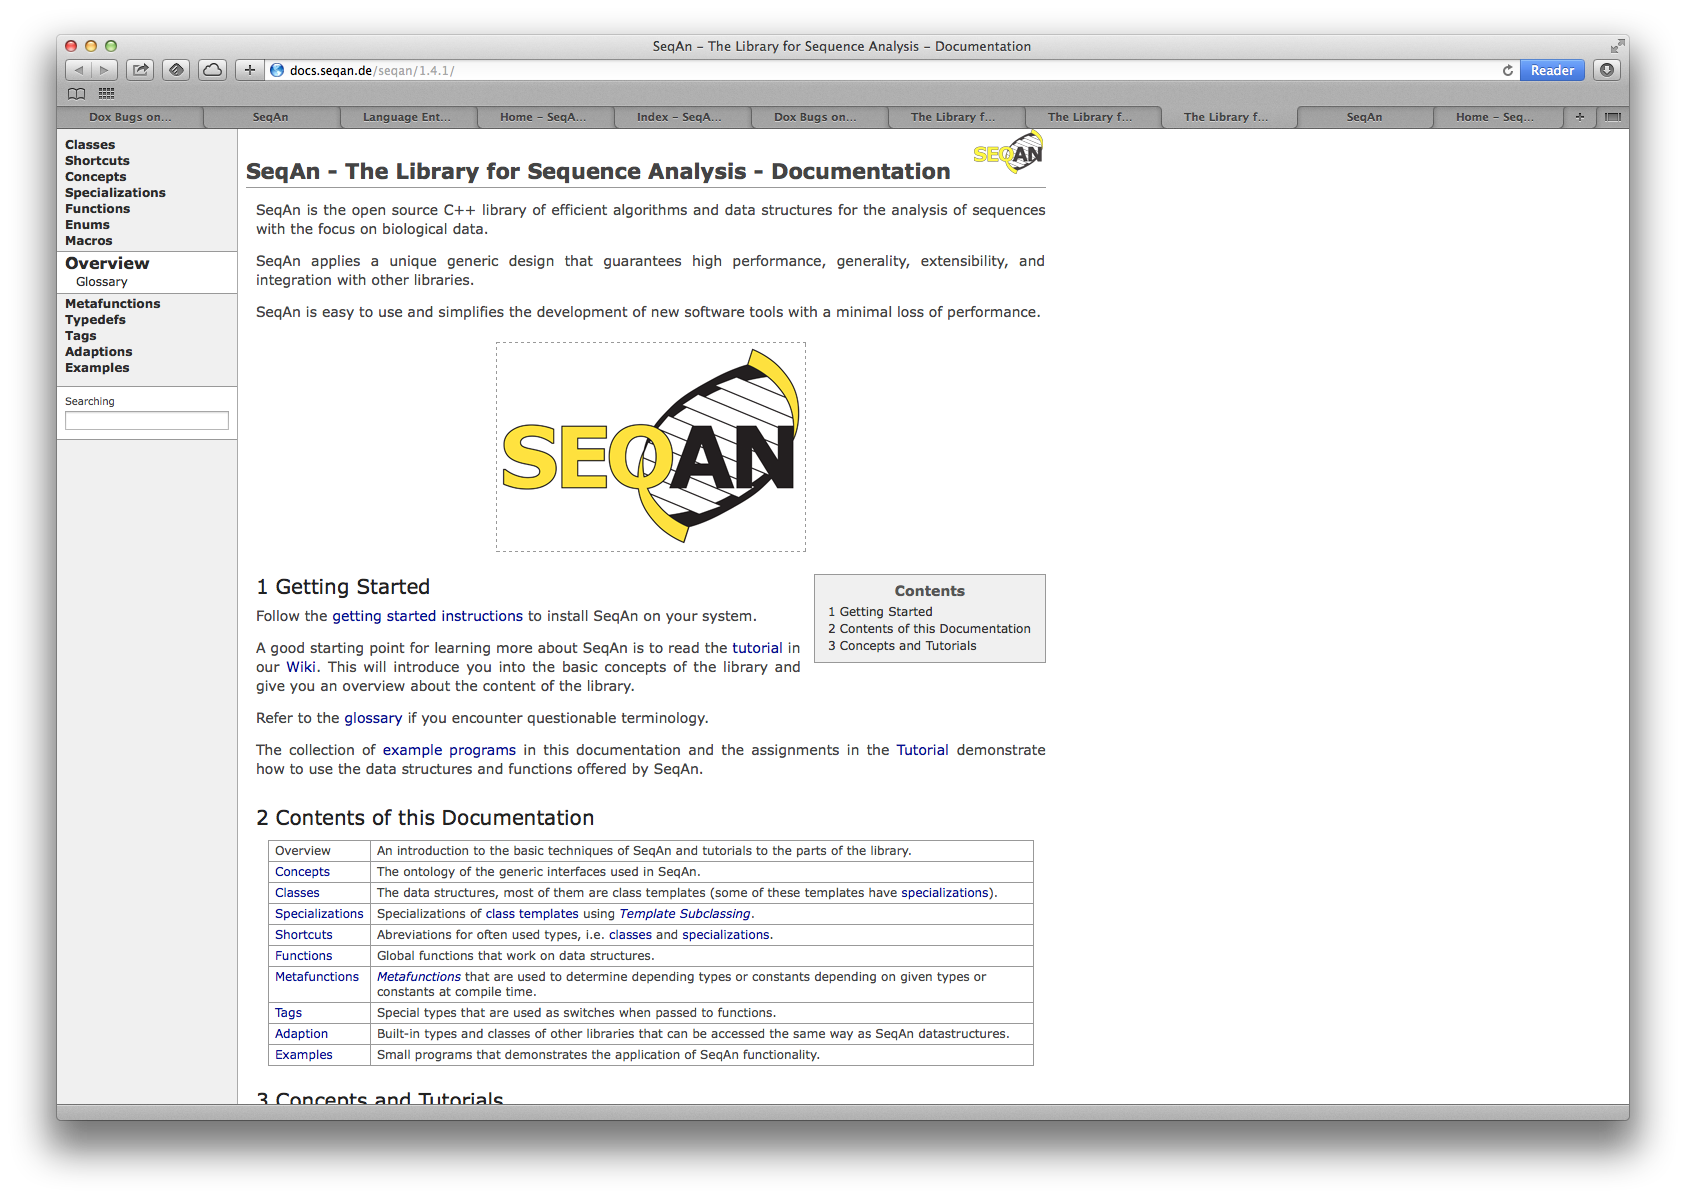
\includegraphics[width=\doxlargewidth]{Figures/dox/dox-1_4_1-large-home.png}
    \caption{Seqan-Online-Dokumentation in Version 1.4.1 - Breite Ansicht - Startseite}
    \label{fig:dox-1_4_1-large-home}
\end{figure}

Donec urna leo, vulputate vitae porta eu, vehicula blandit libero. Phasellus eget massa et leo condimentum mollis. Nullam molestie, justo at pellentesque vulputate, sapien velit ornare diam, nec gravida lacus augue non diam. Integer mattis lacus id libero ultrices sit amet mollis neque molestie. Integer ut leo eget mi volutpat congue. Vivamus sodales, turpis id venenatis placerat, tellus purus adipiscing magna, eu aliquam nibh dolor id nibh. Pellentesque habitant morbi tristique senectus et netus et malesuada fames ac turpis egestas. Sed cursus convallis quam nec vehicula. Sed vulputate neque eget odio fringilla ac sodales urna feugiat.

\begin{figure}
  \centering
    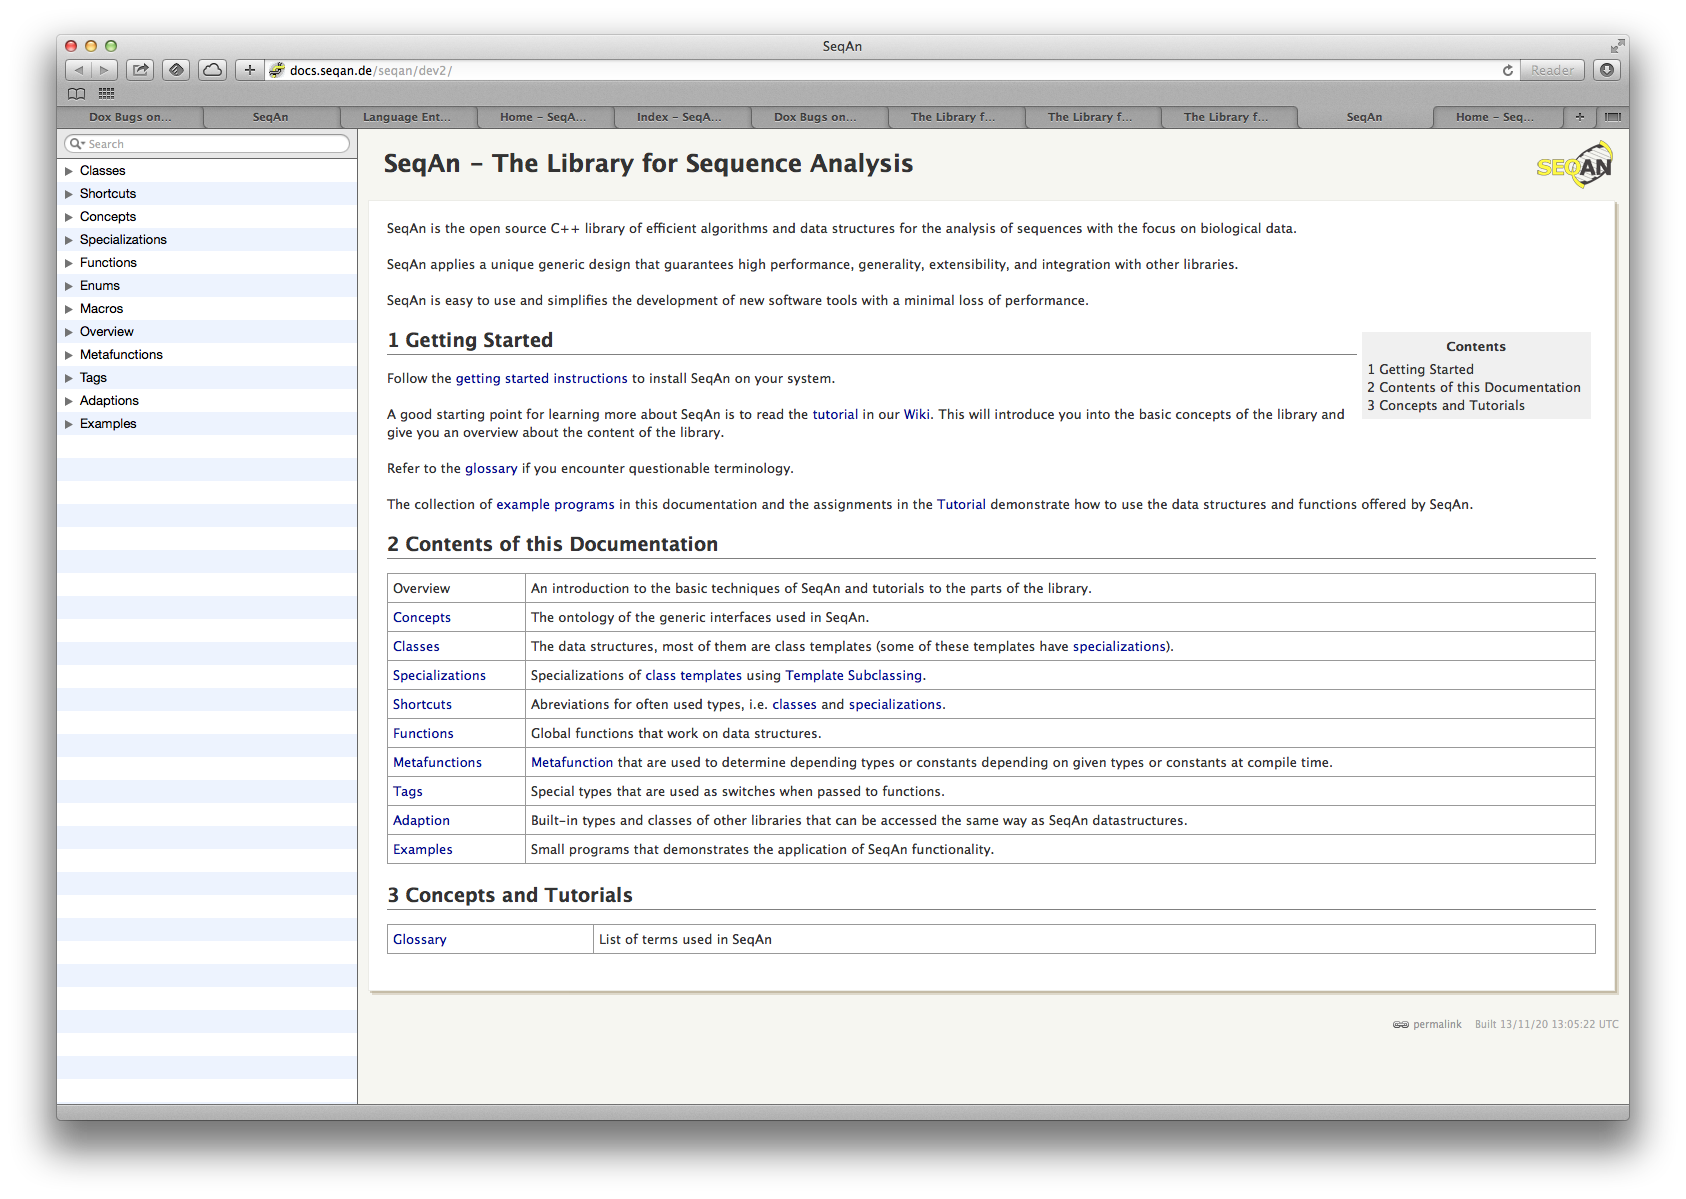
\includegraphics[width=\doxlargewidth]{Figures/dox/dox-2_0_0-large-home.png}
    \caption{Seqan-Online-Dokumentation in Version 2.0 - Breite Ansicht - Startseite}
    \label{fig:dox-2_0_0-large-home}
\end{figure}

\begin{figure}
  \centering
    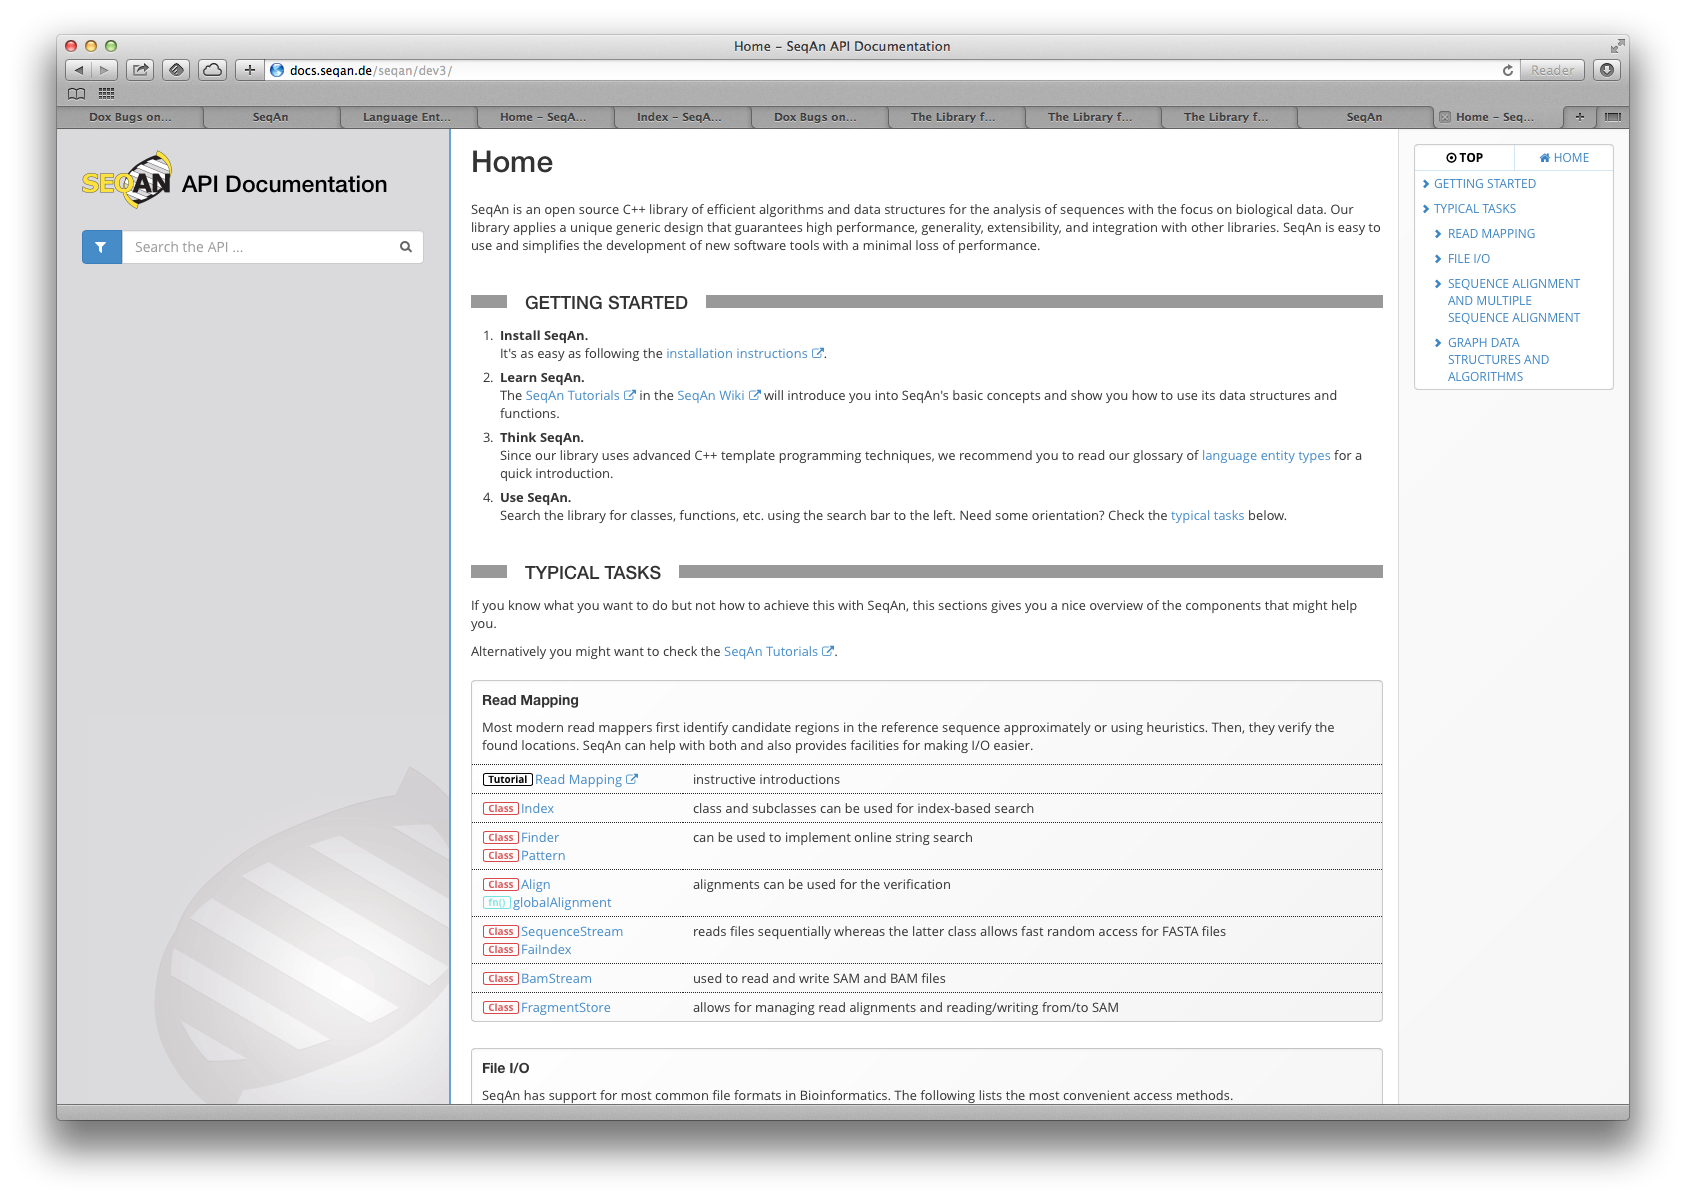
\includegraphics[width=\doxlargewidth]{Figures/dox/dox-3_0_0-large-home.png}
    \caption{Seqan-Online-Dokumentation in Version 3.0 - Breite Ansicht - Startseite}
    \label{fig:dox-3_0_0-large-home}
\end{figure}

Donec urna leo, vulputate vitae porta eu, vehicula blandit libero. Phasellus eget massa et leo condimentum mollis. Nullam molestie, justo at pellentesque vulputate, sapien velit ornare diam, nec gravida lacus augue non diam. Integer mattis lacus id libero ultrices sit amet mollis neque molestie. Integer ut leo eget mi volutpat congue. Vivamus sodales, turpis id venenatis placerat, tellus purus adipiscing magna, eu aliquam nibh dolor id nibh. Pellentesque habitant morbi tristique senectus et netus et malesuada fames ac turpis egestas. Sed cursus convallis quam nec vehicula. Sed vulputate neque eget odio fringilla ac sodales urna feugiat.

Donec urna leo, vulputate vitae porta eu, vehicula blandit libero. Phasellus eget massa et leo condimentum mollis. Nullam molestie, justo at pellentesque vulputate, sapien velit ornare diam, nec gravida lacus augue non diam. Integer mattis lacus id libero ultrices sit amet mollis neque molestie. Integer ut leo eget mi volutpat congue. Vivamus sodales, turpis id venenatis placerat, tellus purus adipiscing magna, eu aliquam nibh dolor id nibh. Pellentesque habitant morbi tristique senectus et netus et malesuada fames ac turpis egestas. Sed cursus convallis quam nec vehicula. Sed vulputate neque eget odio fringilla ac sodales urna feugiat.


\begin{figure}
  \centering
    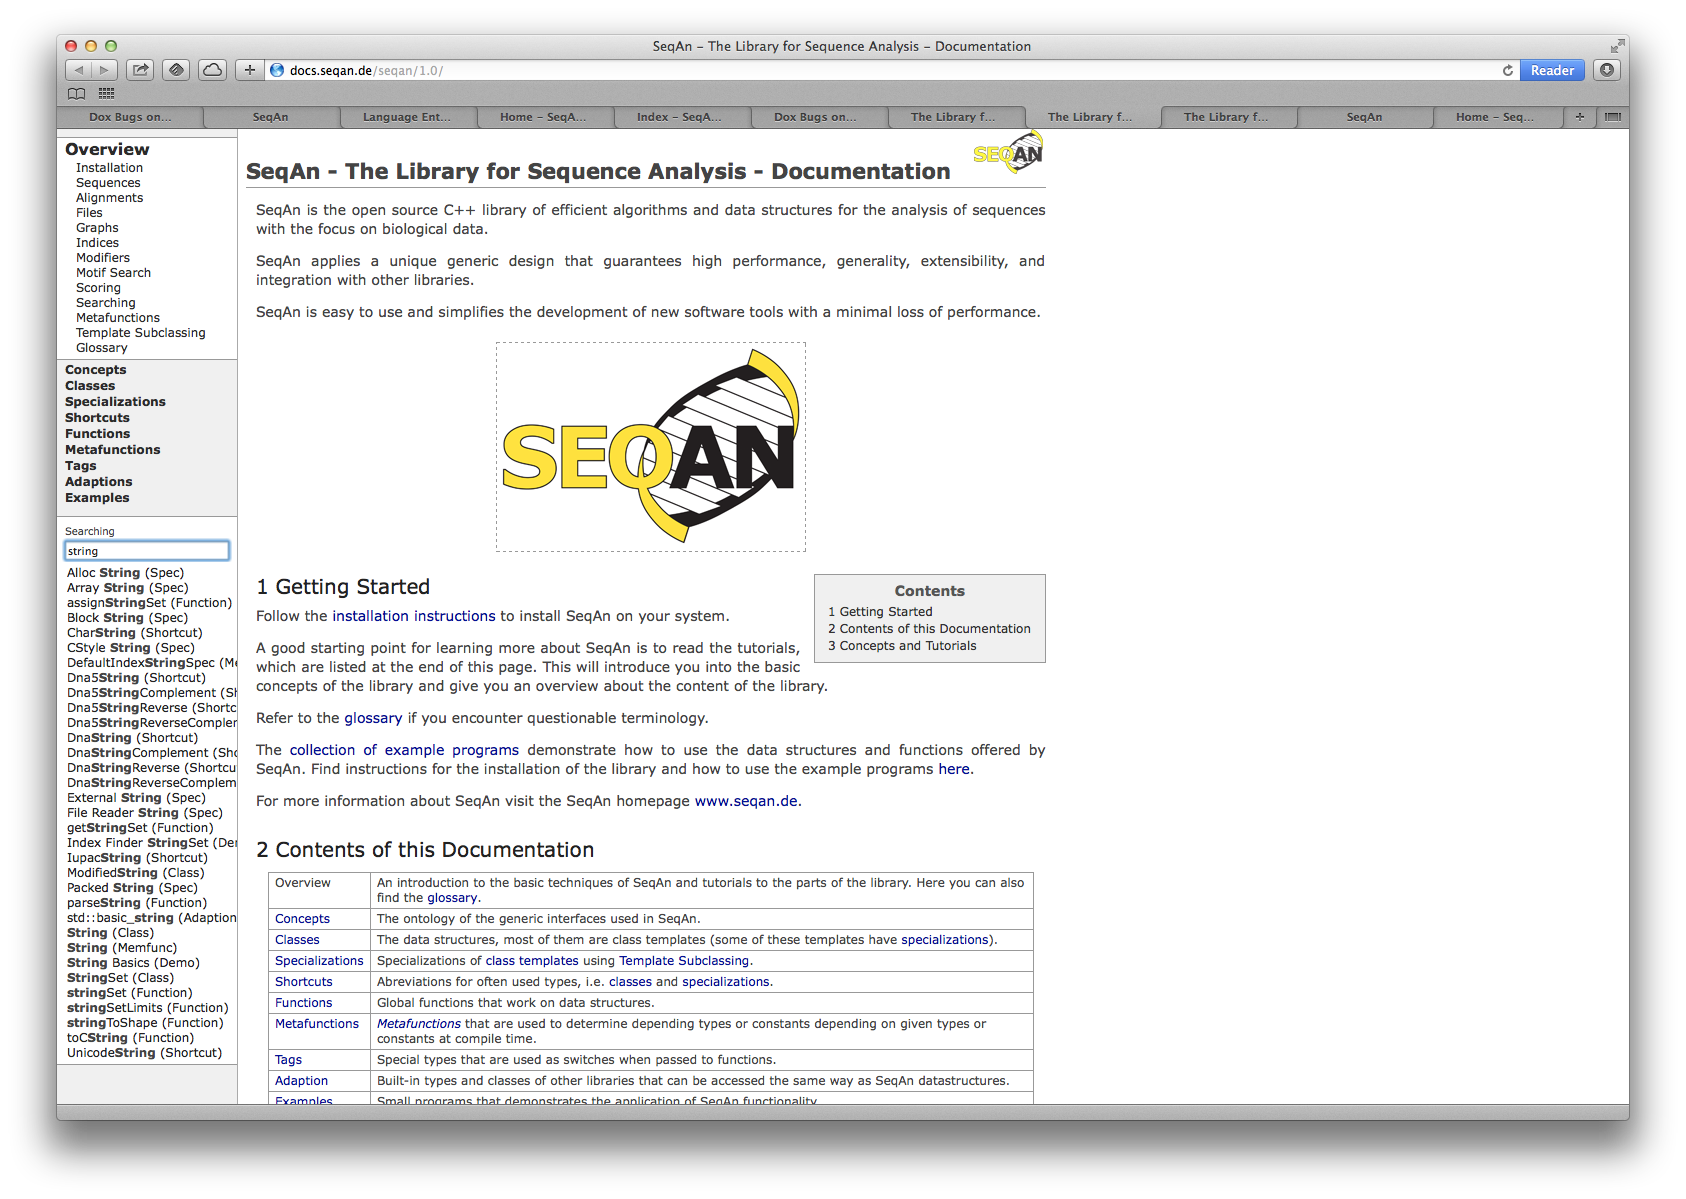
\includegraphics[width=\doxlargewidth]{Figures/dox/dox-1_0_0-large-string.png}
    \caption{Seqan-Online-Dokumentation in Version 1.0 - Breite Ansicht - Suche nach ``String''}
    \label{fig:dox-1_0_0-large-string}
\end{figure}

\begin{figure}
  \centering
    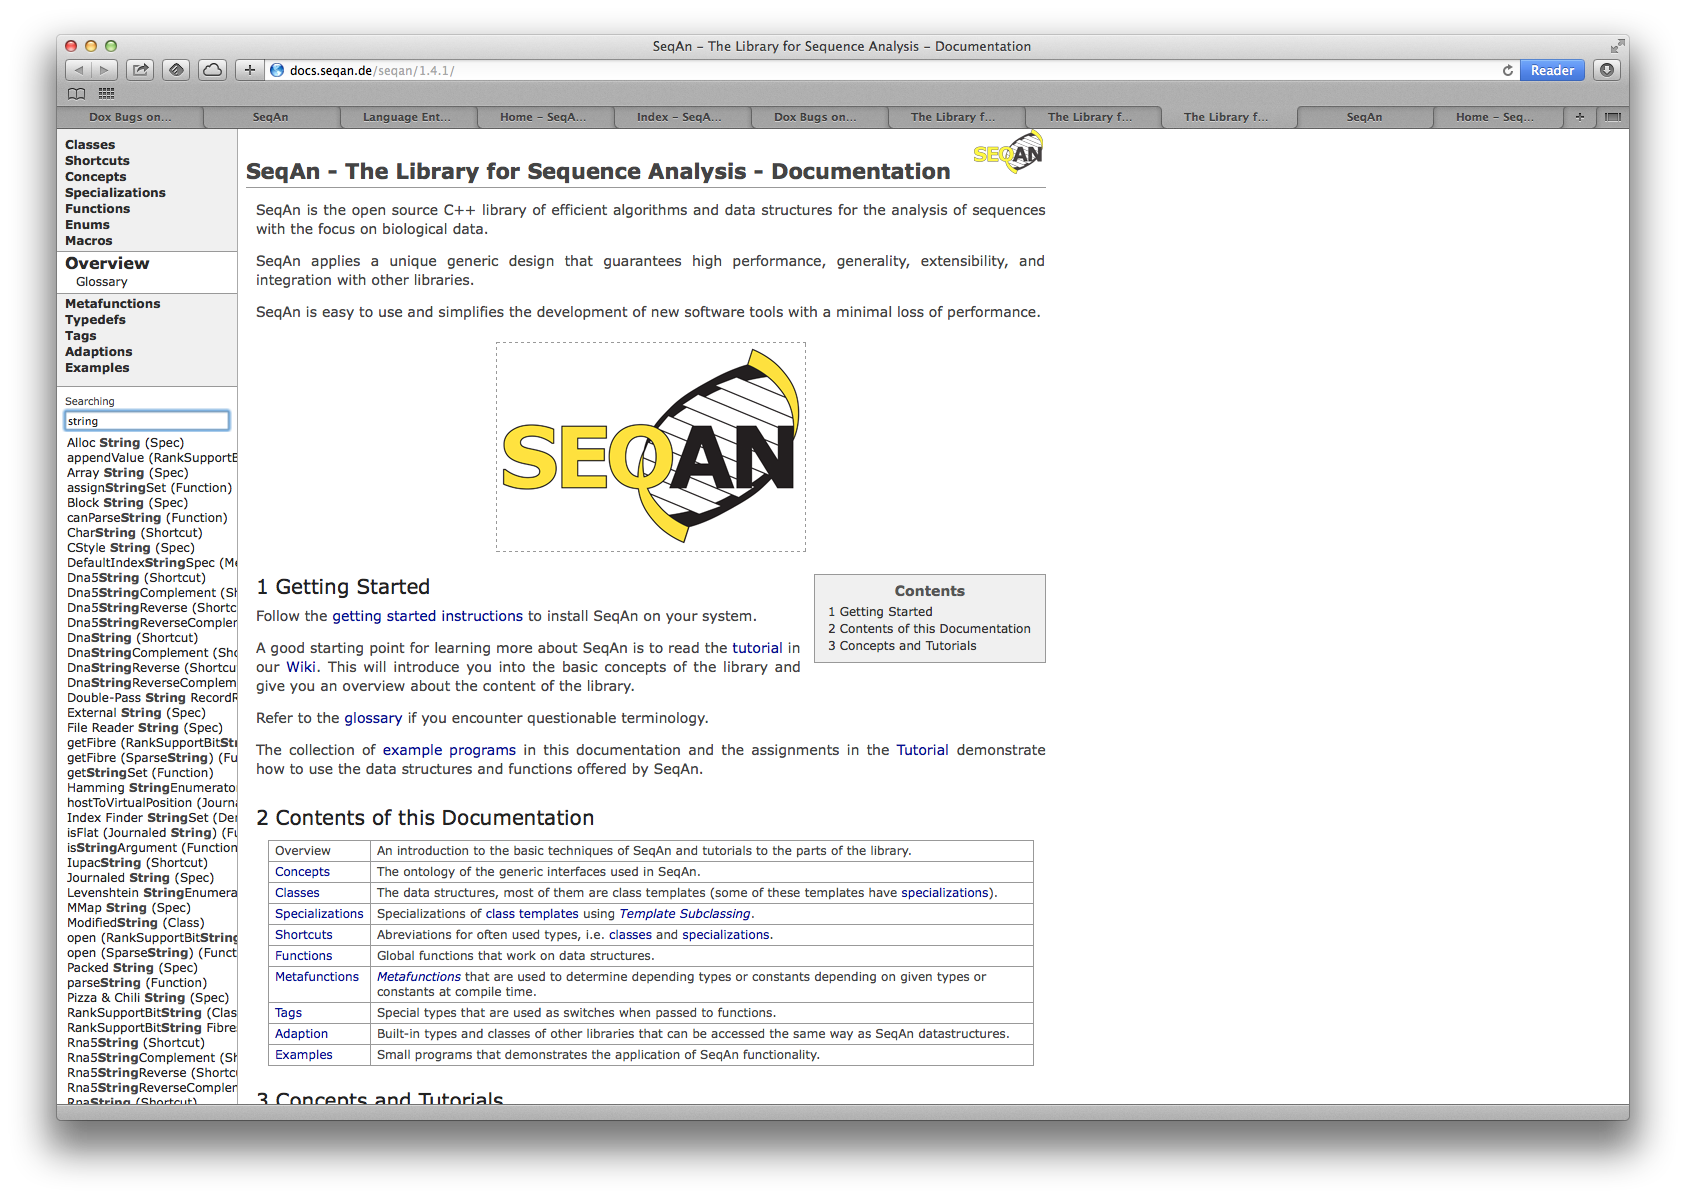
\includegraphics[width=\doxlargewidth]{Figures/dox/dox-1_4_1-large-string.png}
    \caption{Seqan-Online-Dokumentation in Version 1.4.1 - Breite Ansicht - Suche nach ``String''}
    \label{fig:dox-1_4_1-large-string}
\end{figure}

Donec urna leo, vulputate vitae porta eu, vehicula blandit libero. Phasellus eget massa et leo condimentum mollis. Nullam molestie, justo at pellentesque vulputate, sapien velit ornare diam, nec gravida lacus augue non diam. Integer mattis lacus id libero ultrices sit amet mollis neque molestie. Integer ut leo eget mi volutpat congue. Vivamus sodales, turpis id venenatis placerat, tellus purus adipiscing magna, eu aliquam nibh dolor id nibh. Pellentesque habitant morbi tristique senectus et netus et malesuada fames ac turpis egestas. Sed cursus convallis quam nec vehicula. Sed vulputate neque eget odio fringilla ac sodales urna feugiat.

\begin{figure}
  \centering
    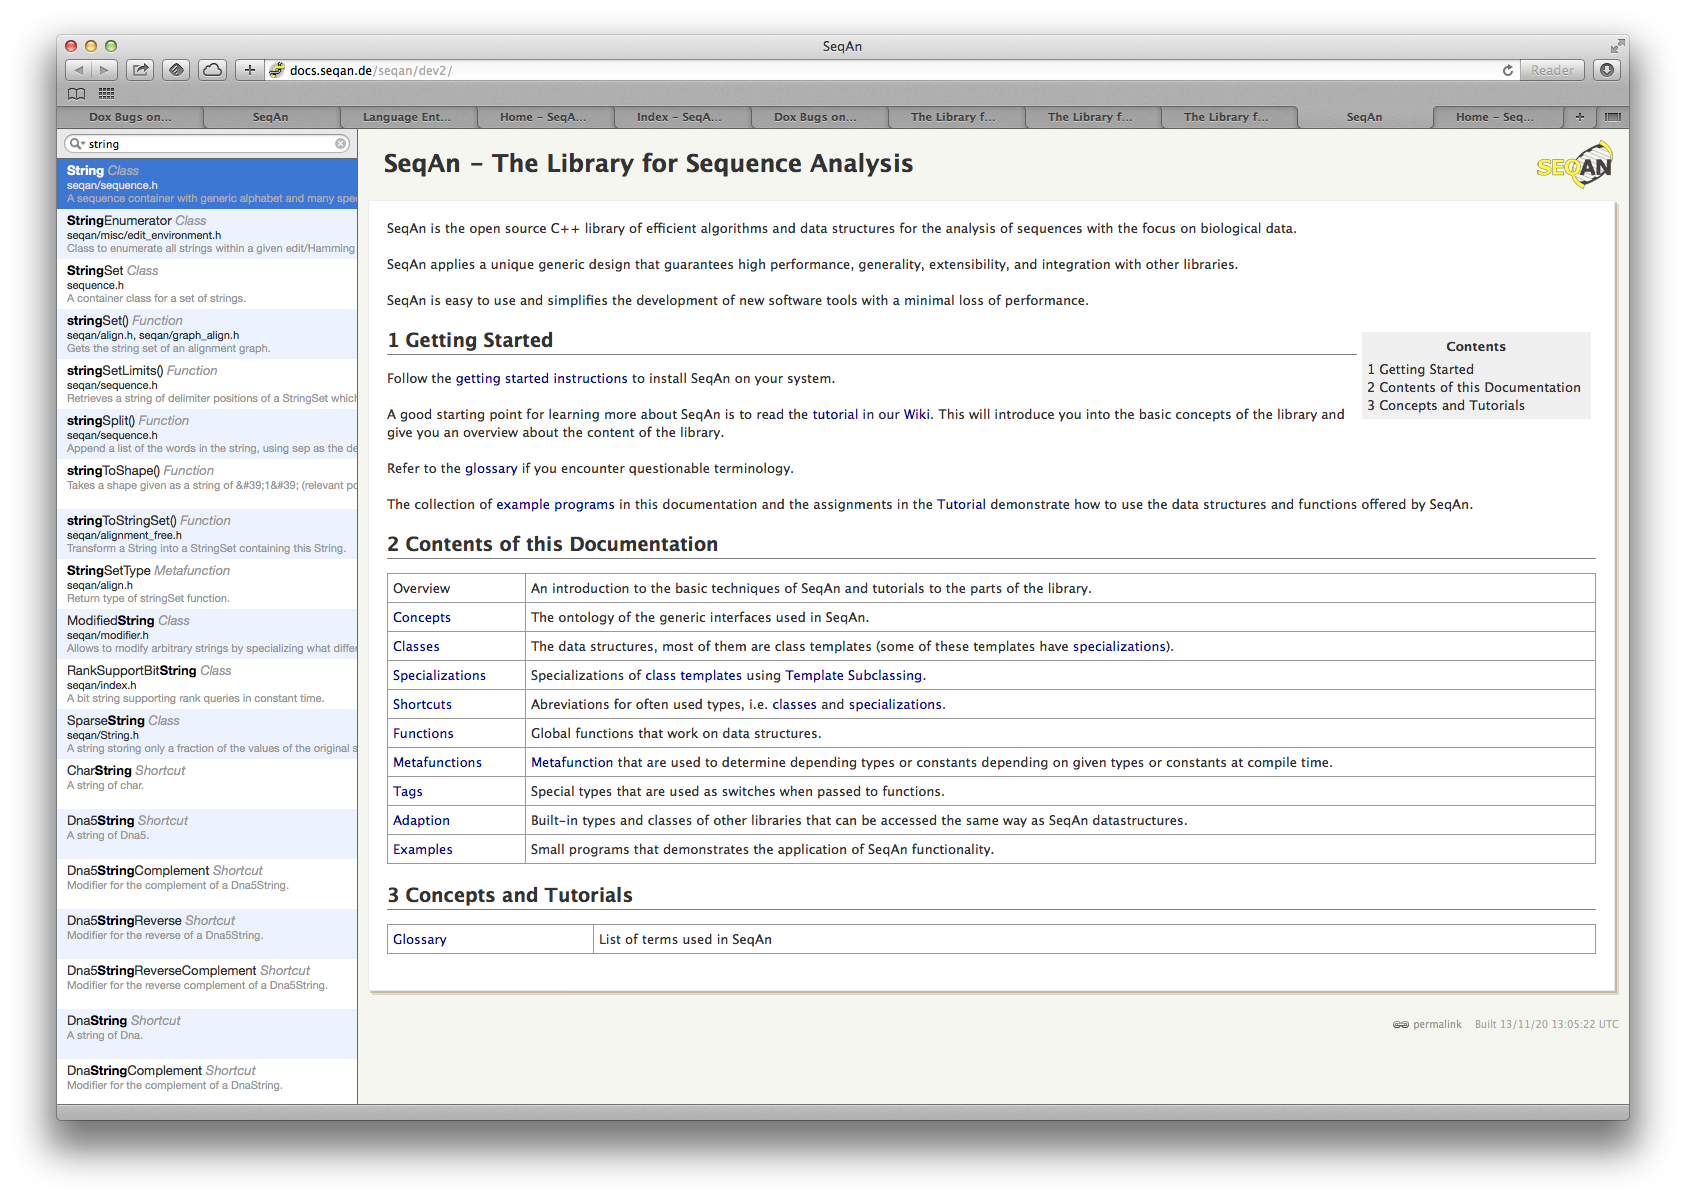
\includegraphics[width=\doxlargewidth]{Figures/dox/dox-2_0_0-large-string.png}
    \caption{Seqan-Online-Dokumentation in Version 2.0 - Breite Ansicht - Suche nach ``String''}
    \label{fig:dox-2_0_0-large-string}
\end{figure}

\begin{figure}
  \centering
    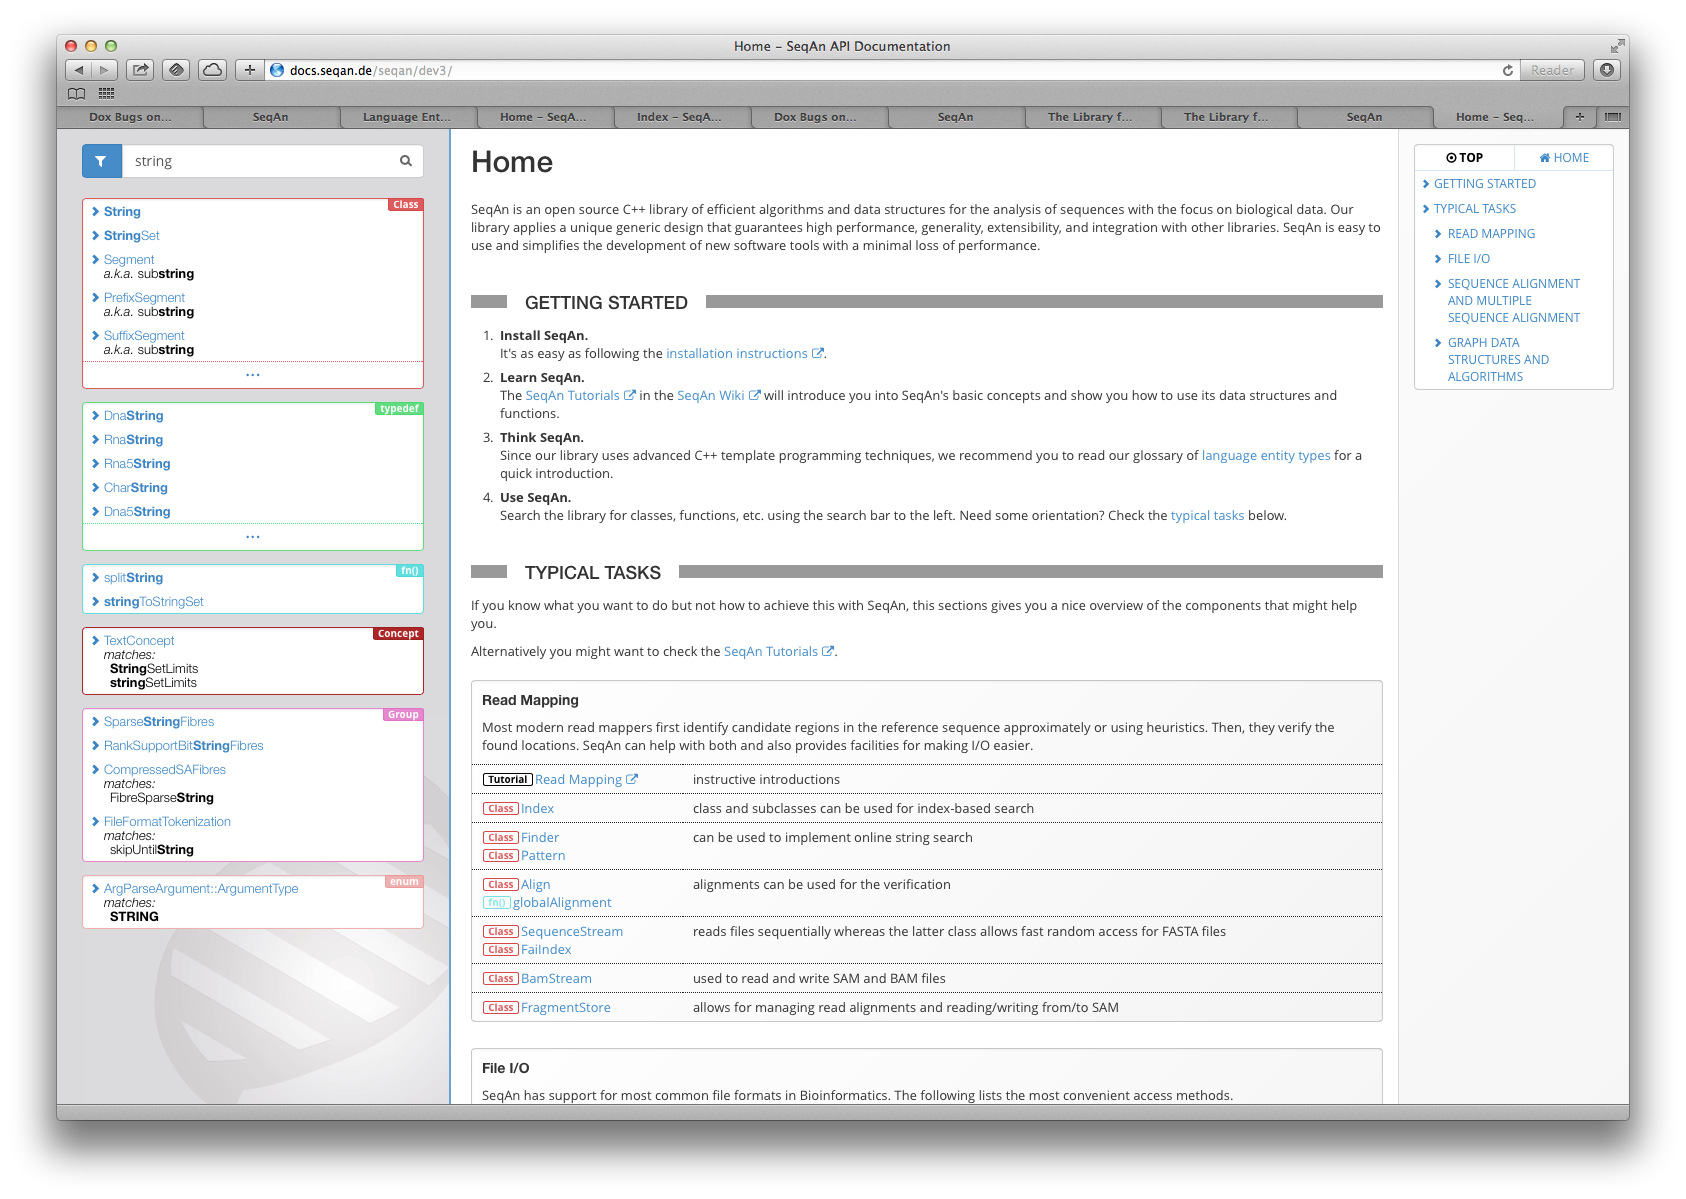
\includegraphics[width=\doxlargewidth]{Figures/dox/dox-3_0_0-large-string.png}
    \caption{Seqan-Online-Dokumentation in Version 3.0 - Breite Ansicht - Suche nach ``String''}
    \label{fig:dox-3_0_0-large-string}
\end{figure}

Donec urna leo, vulputate vitae porta eu, vehicula blandit libero. Phasellus eget massa et leo condimentum mollis. Nullam molestie, justo at pellentesque vulputate, sapien velit ornare diam, nec gravida lacus augue non diam. Integer mattis lacus id libero ultrices sit amet mollis neque molestie. Integer ut leo eget mi volutpat congue. Vivamus sodales, turpis id venenatis placerat, tellus purus adipiscing magna, eu aliquam nibh dolor id nibh. Pellentesque habitant morbi tristique senectus et netus et malesuada fames ac turpis egestas. Sed cursus convallis quam nec vehicula. Sed vulputate neque eget odio fringilla ac sodales urna feugiat.

\begin{figure}
  \centering
    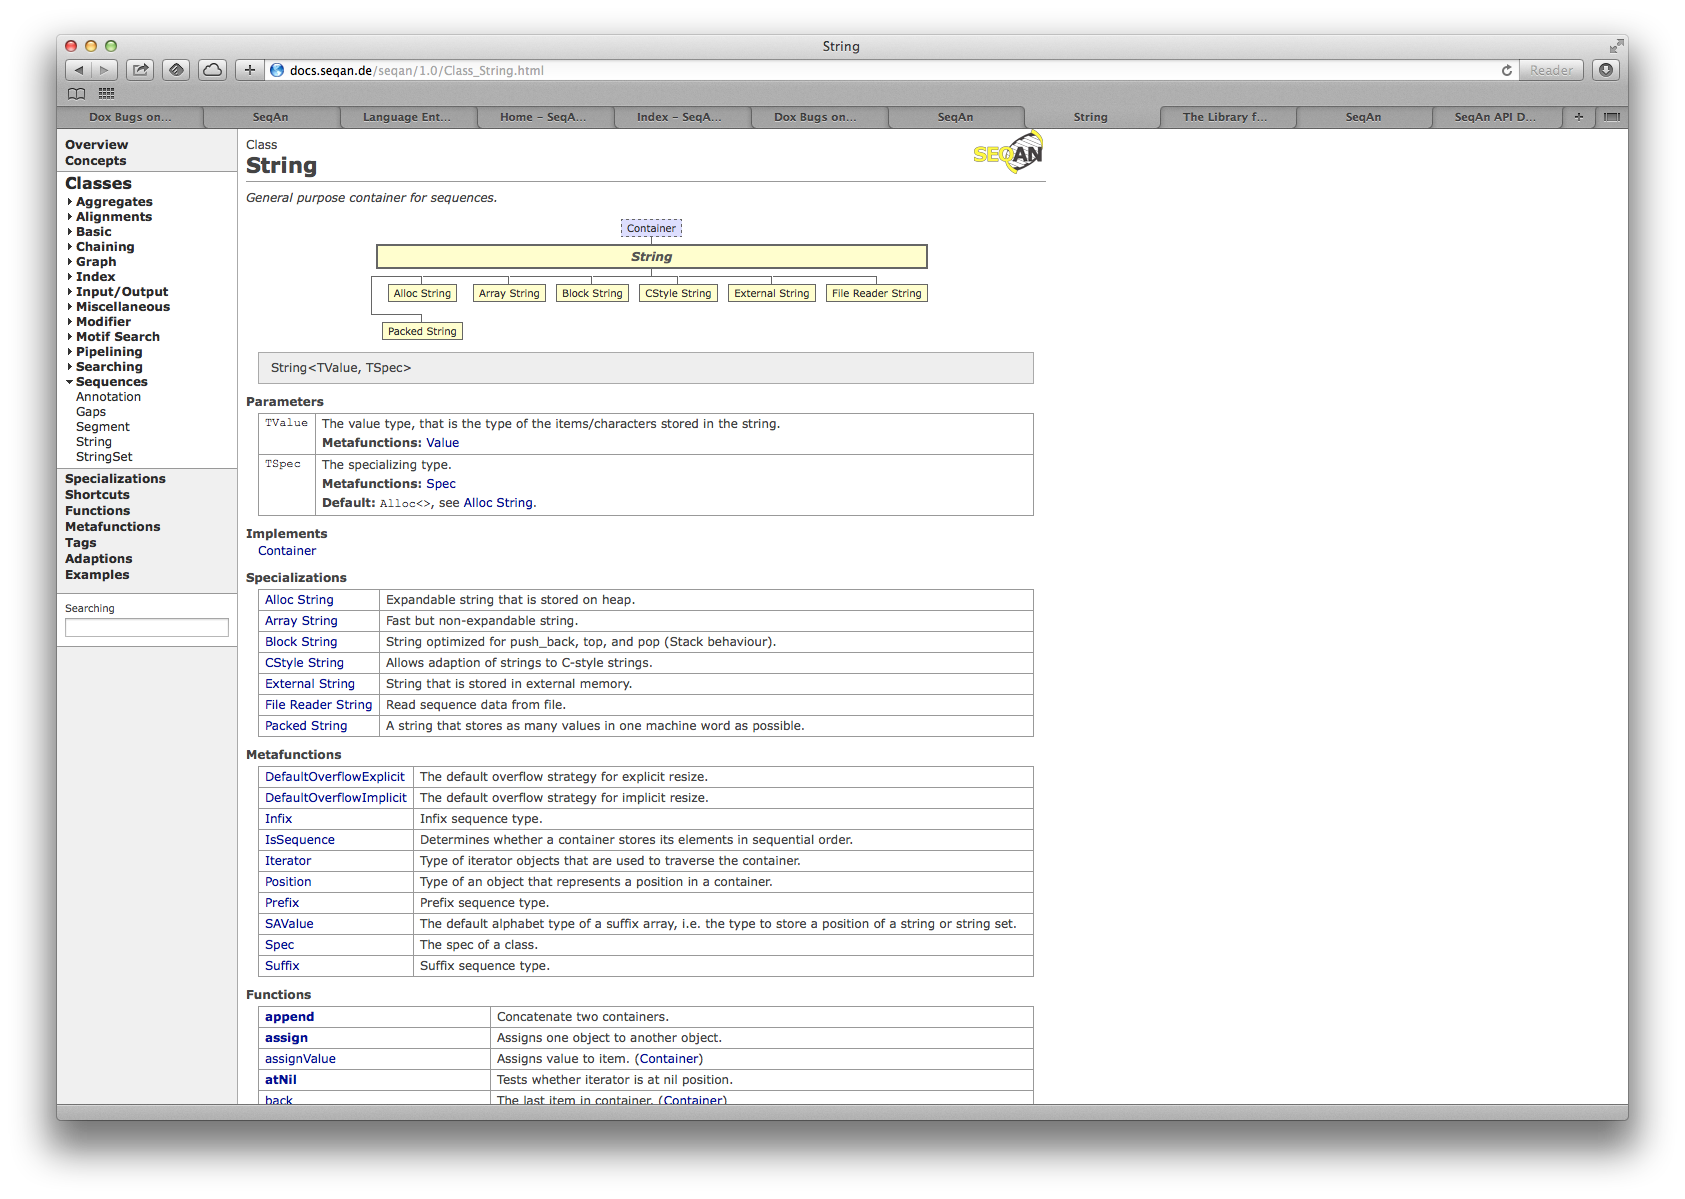
\includegraphics[width=\doxlargewidth]{Figures/dox/dox-1_0_0-large-string-opened.png}
    \caption{Seqan-Online-Dokumentation in Version 1.0 - Breite Ansicht - Klasse ``String''}
    \label{fig:dox-1_0_0-large-string-opened}
\end{figure}

\begin{figure}
  \centering
    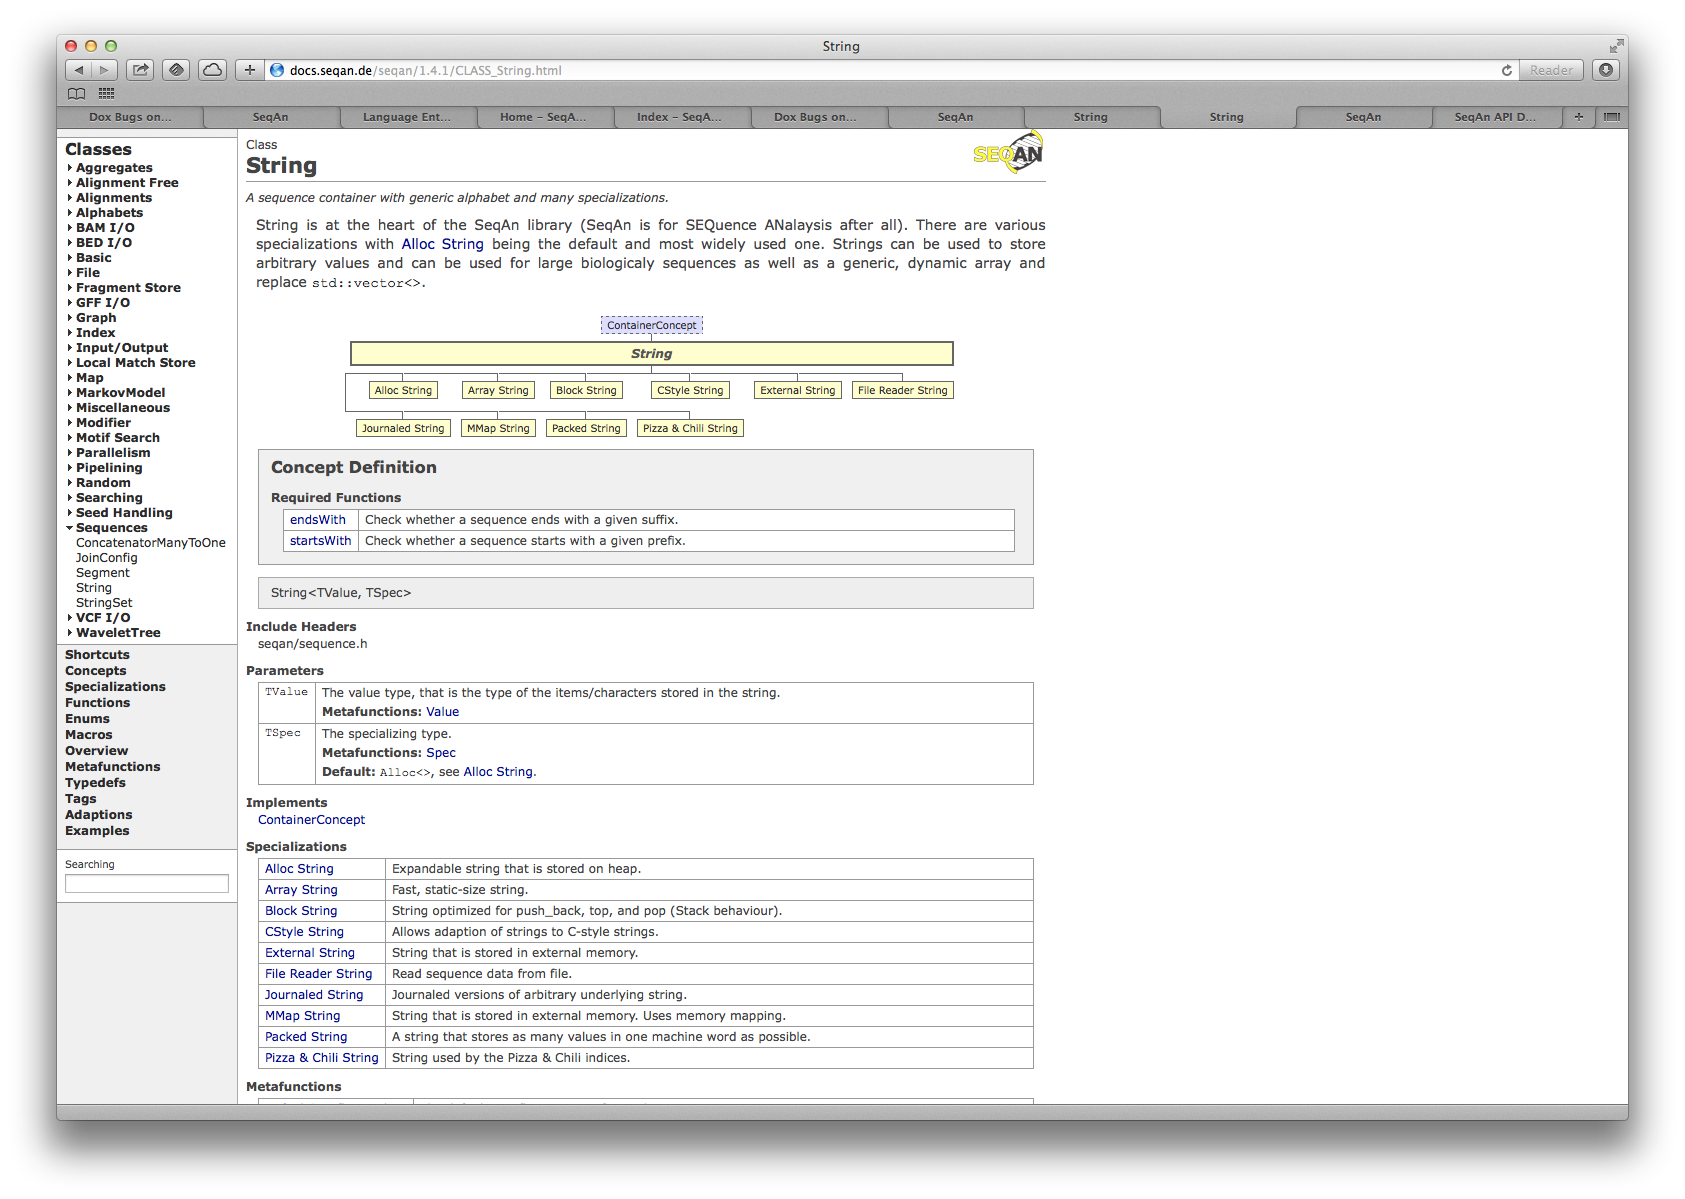
\includegraphics[width=\doxlargewidth]{Figures/dox/dox-1_4_1-large-string-opened.png}
    \caption{Seqan-Online-Dokumentation in Version 1.4.1 - Breite Ansicht - Klasse ``String''}
    \label{fig:dox-1_4_1-large-string-opened}
\end{figure}

Donec urna leo, vulputate vitae porta eu, vehicula blandit libero. Phasellus eget massa et leo condimentum mollis. Nullam molestie, justo at pellentesque vulputate, sapien velit ornare diam, nec gravida lacus augue non diam. Integer mattis lacus id libero ultrices sit amet mollis neque molestie. Integer ut leo eget mi volutpat congue. Vivamus sodales, turpis id venenatis placerat, tellus purus adipiscing magna, eu aliquam nibh dolor id nibh. Pellentesque habitant morbi tristique senectus et netus et malesuada fames ac turpis egestas. Sed cursus convallis quam nec vehicula. Sed vulputate neque eget odio fringilla ac sodales urna feugiat.

Donec urna leo, vulputate vitae porta eu, vehicula blandit libero. Phasellus eget massa et leo condimentum mollis. Nullam molestie, justo at pellentesque vulputate, sapien velit ornare diam, nec gravida lacus augue non diam. Integer mattis lacus id libero ultrices sit amet mollis neque molestie. Integer ut leo eget mi volutpat congue. Vivamus sodales, turpis id venenatis placerat, tellus purus adipiscing magna, eu aliquam nibh dolor id nibh. Pellentesque habitant morbi tristique senectus et netus et malesuada fames ac turpis egestas. Sed cursus convallis quam nec vehicula. Sed vulputate neque eget odio fringilla ac sodales urna feugiat.

\begin{figure}
  \centering
    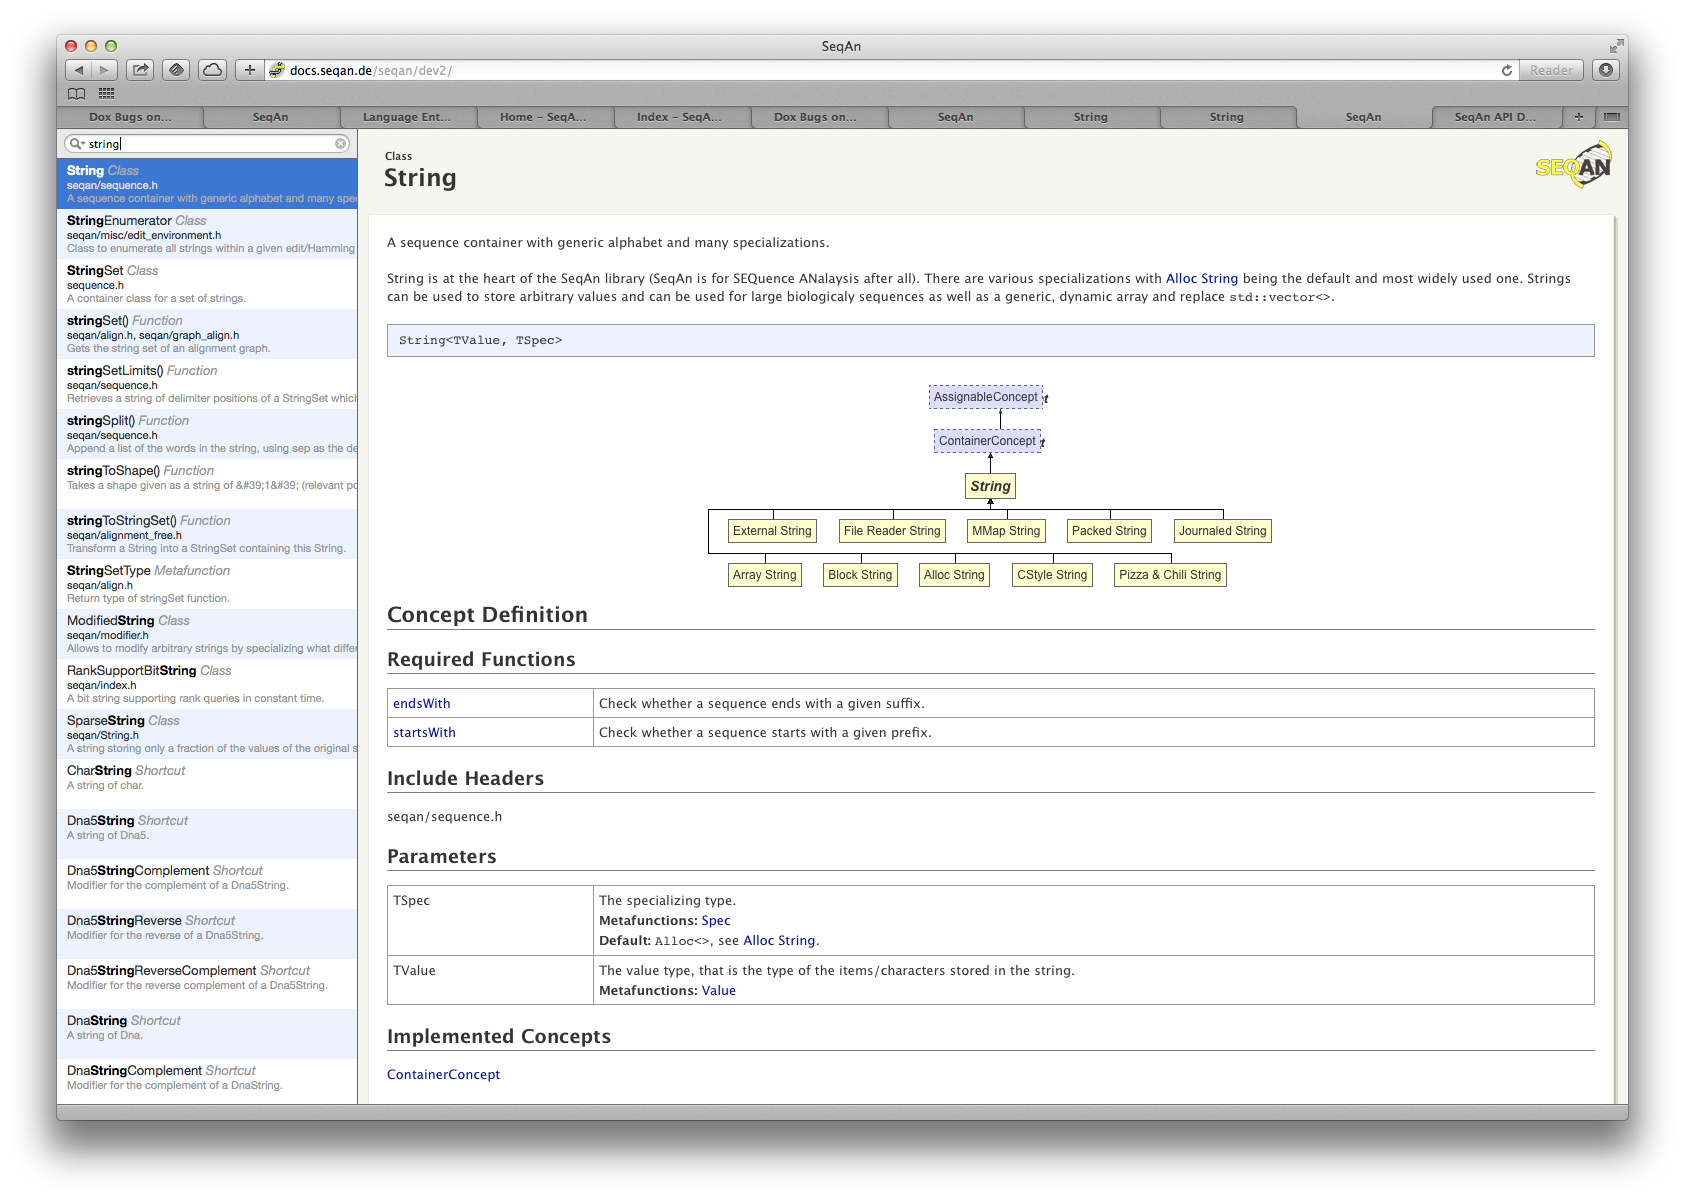
\includegraphics[width=\doxlargewidth]{Figures/dox/dox-2_0_0-large-string-opened.png}
    \caption{Seqan-Online-Dokumentation in Version 2.0 - Breite Ansicht - Klasse ``String''}
    \label{fig:dox-2_0_0-large-string-opened}
\end{figure}

\begin{figure}
  \centering
    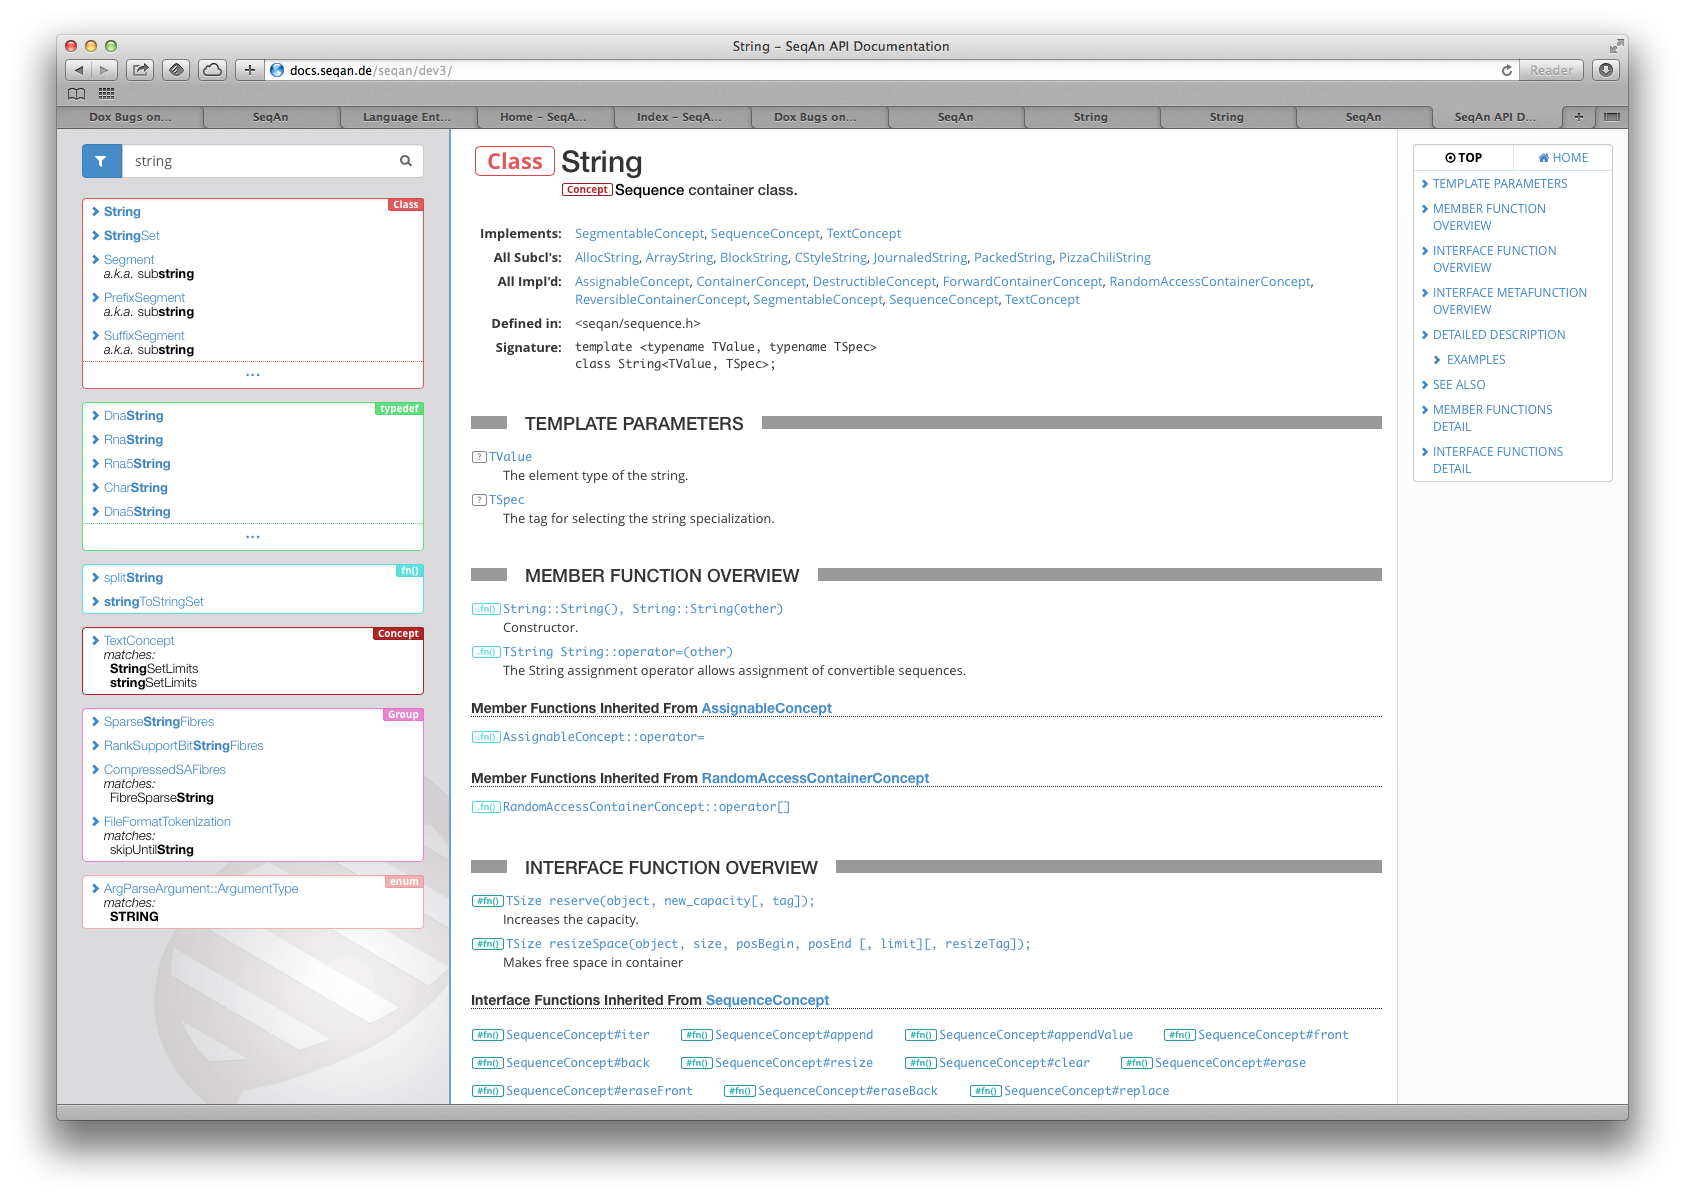
\includegraphics[width=\doxlargewidth]{Figures/dox/dox-3_0_0-large-string-opened.png}
    \caption{Seqan-Online-Dokumentation in Version 3.0 - Breite Ansicht - Klasse ``String''}
    \label{fig:dox-3_0_0-large-string-opened}
\end{figure}

Donec urna leo, vulputate vitae porta eu, vehicula blandit libero. Phasellus eget massa et leo condimentum mollis. Nullam molestie, justo at pellentesque vulputate, sapien velit ornare diam, nec gravida lacus augue non diam. Integer mattis lacus id libero ultrices sit amet mollis neque molestie. Integer ut leo eget mi volutpat congue. Vivamus sodales, turpis id venenatis placerat, tellus purus adipiscing magna, eu aliquam nibh dolor id nibh. Pellentesque habitant morbi tristique senectus et netus et malesuada fames ac turpis egestas. Sed cursus convallis quam nec vehicula. Sed vulputate neque eget odio fringilla ac sodales urna feugiat.

Donec urna leo, vulputate vitae porta eu, vehicula blandit libero. Phasellus eget massa et leo condimentum mollis. Nullam molestie, justo at pellentesque vulputate, sapien velit ornare diam, nec gravida lacus augue non diam. Integer mattis lacus id libero ultrices sit amet mollis neque molestie. Integer ut leo eget mi volutpat congue. Vivamus sodales, turpis id venenatis placerat, tellus purus adipiscing magna, eu aliquam nibh dolor id nibh. Pellentesque habitant morbi tristique senectus et netus et malesuada fames ac turpis egestas. Sed cursus convallis quam nec vehicula. Sed vulputate neque eget odio fringilla ac sodales urna feugiat.

\begin{figure}
  \centering
    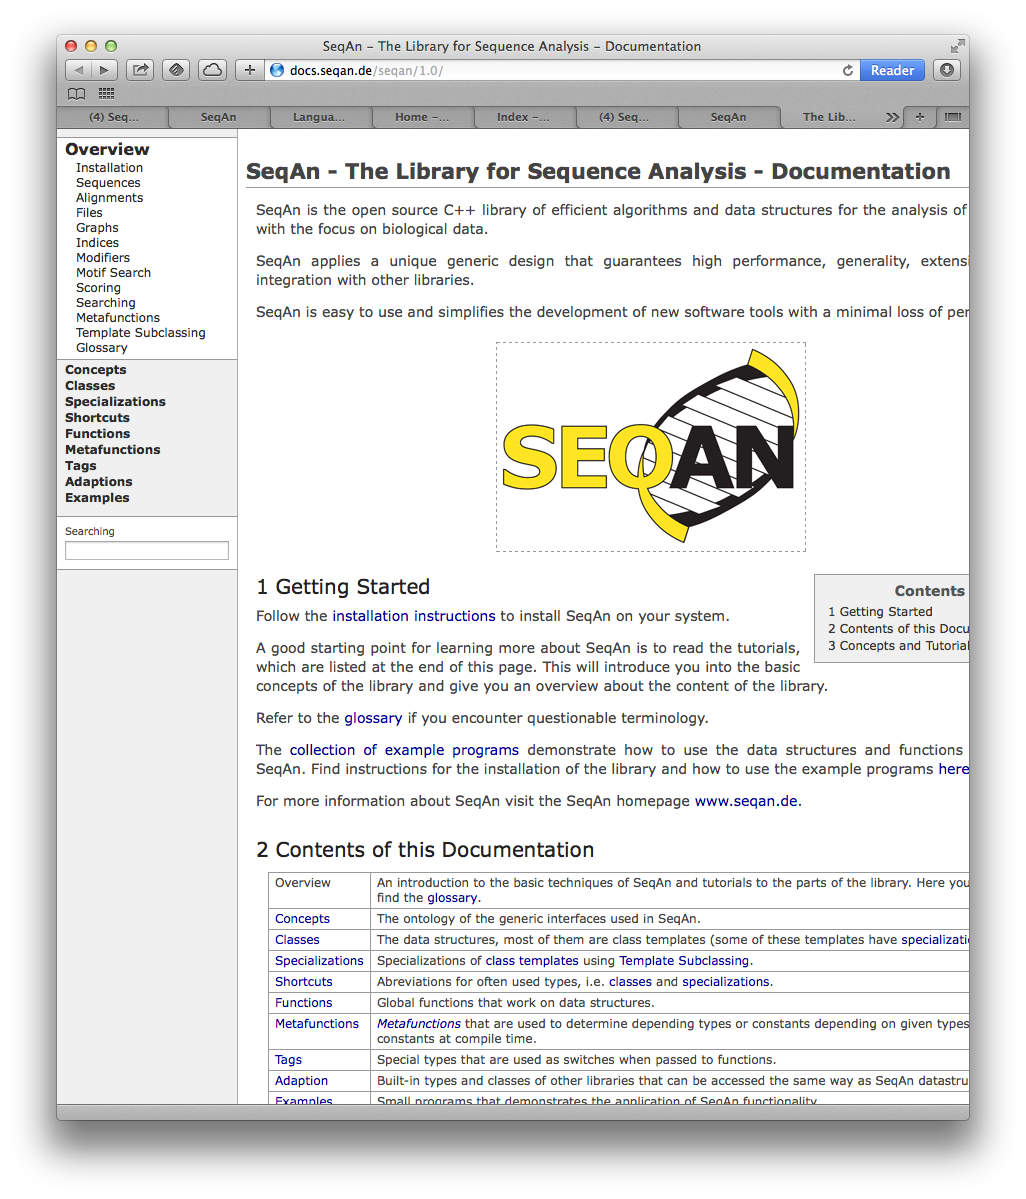
\includegraphics[width=\doxnarrowwidth]{Figures/dox/dox-1_0_0-small-home.png}
    \caption{Seqan-Online-Dokumentation in Version 1.0 - Smale Ansicht - Startseite}
    \label{fig:dox-1_0_0-small-home}
\end{figure}

\begin{figure}
  \centering
    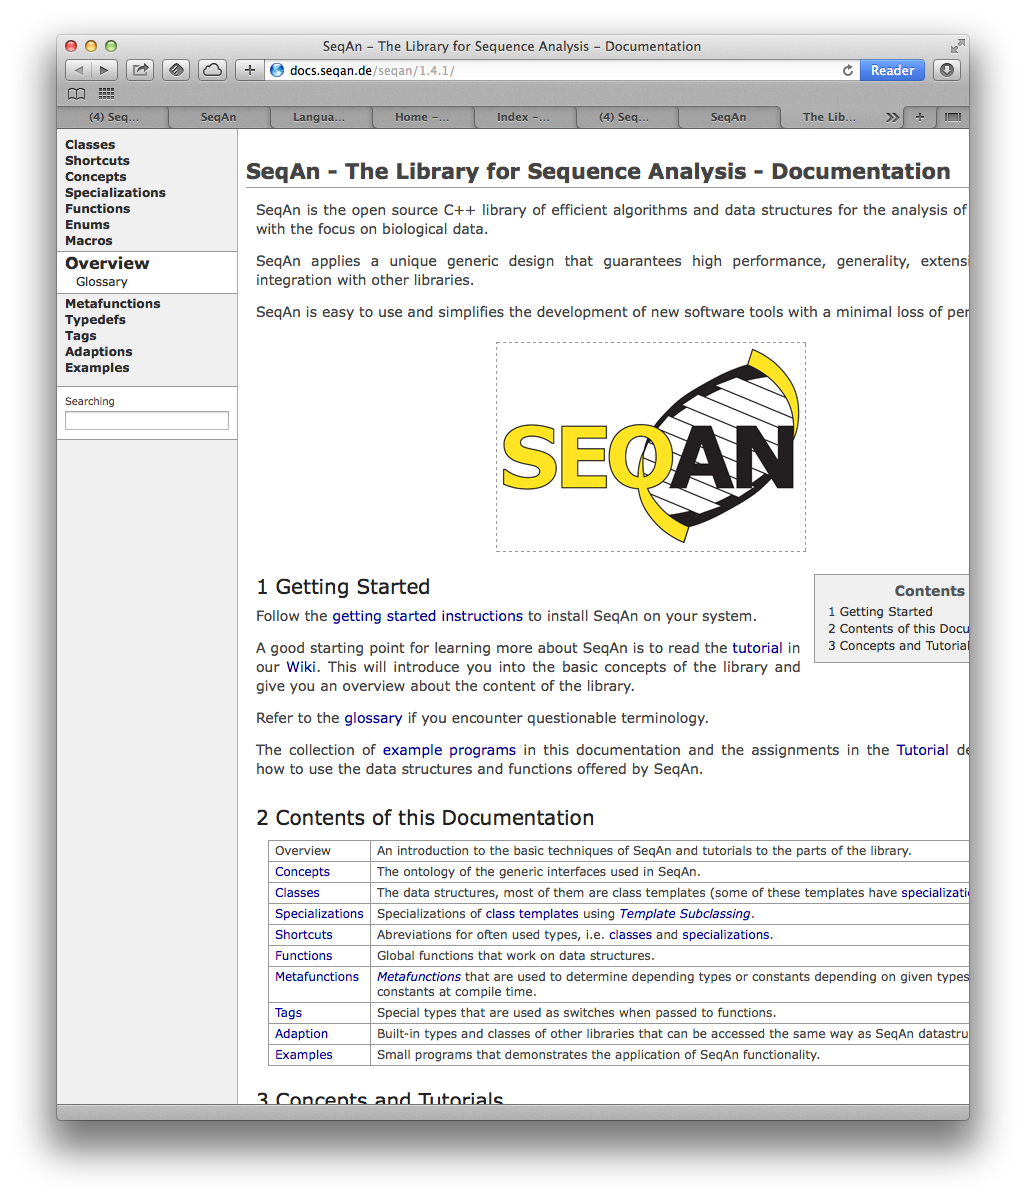
\includegraphics[width=\doxnarrowwidth]{Figures/dox/dox-1_4_1-small-home.png}
    \caption{Seqan-Online-Dokumentation in Version 1.4.1 - Smale Ansicht - Startseite}
    \label{fig:dox-1_4_1-small-home}
\end{figure}

\begin{figure}
  \centering
    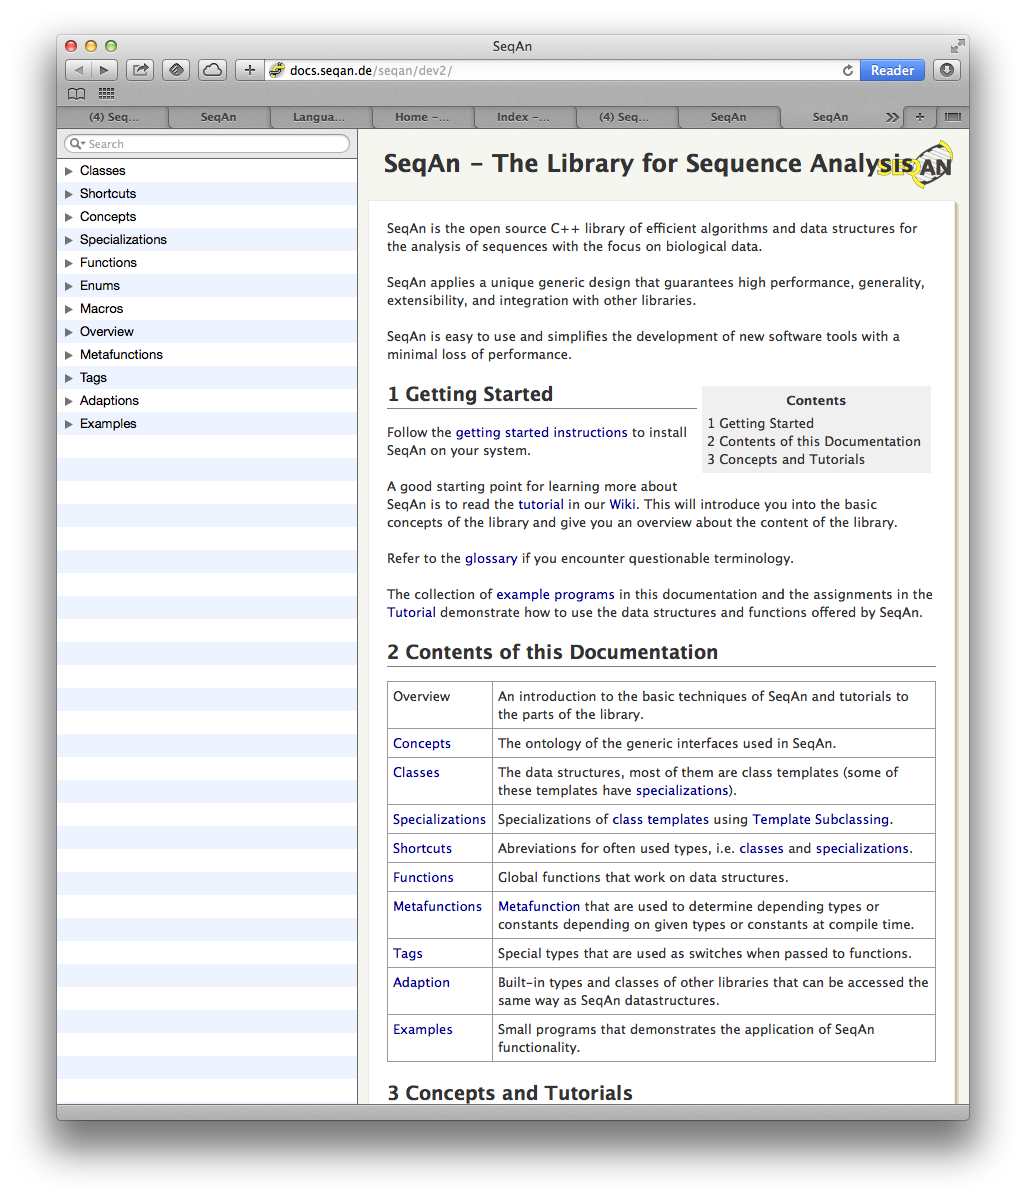
\includegraphics[width=\doxnarrowwidth]{Figures/dox/dox-2_0_0-small-home.png}
    \caption{Seqan-Online-Dokumentation in Version 2.0 - Smale Ansicht - Startseite}
    \label{fig:dox-2_0_0-small-home}
\end{figure}

\begin{figure}
  \centering
    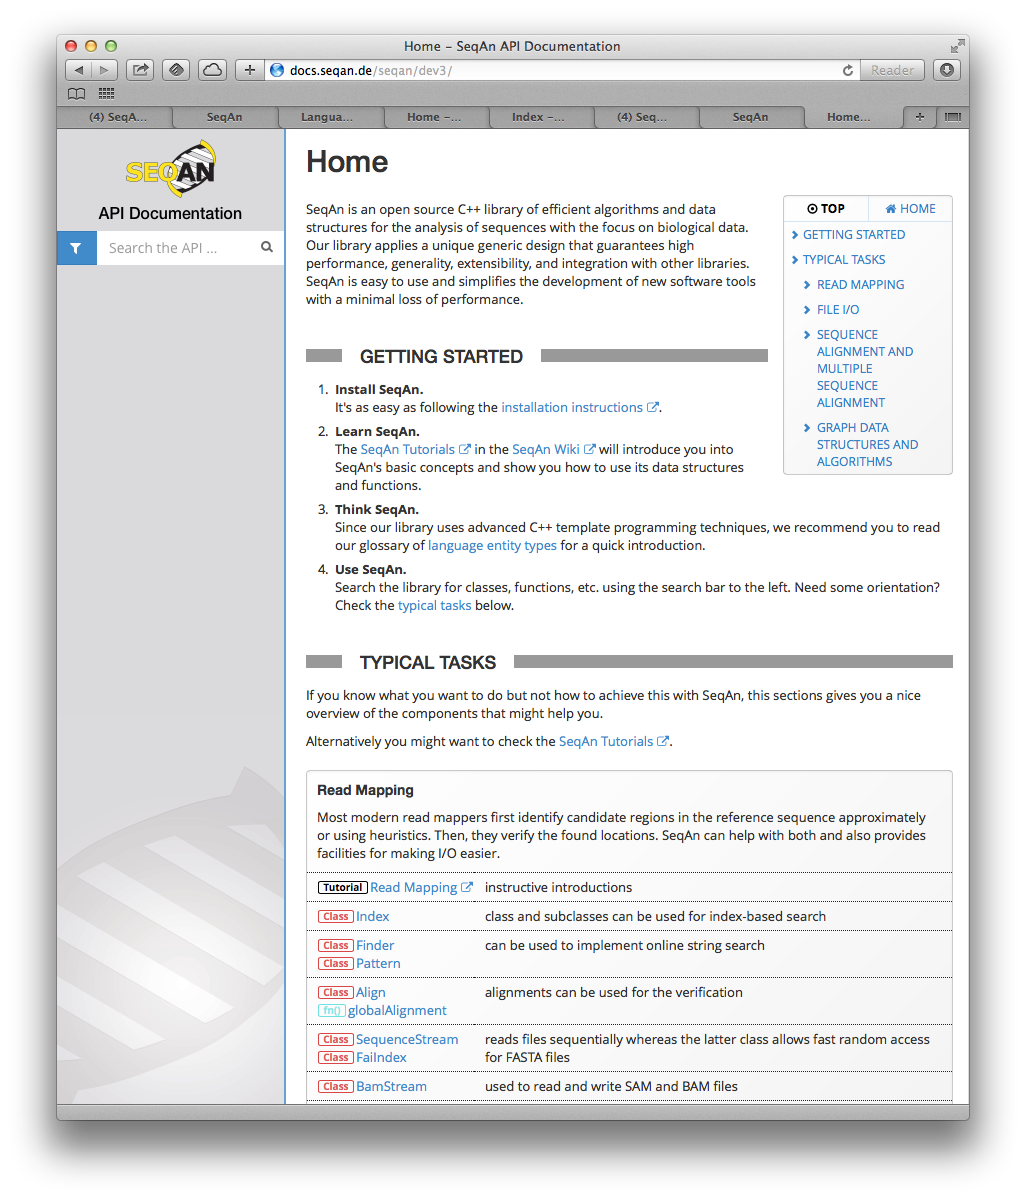
\includegraphics[width=\doxnarrowwidth]{Figures/dox/dox-3_0_0-small-home.png}
    \caption{Seqan-Online-Dokumentation in Version 3.0 - Smale Ansicht - Startseite}
    \label{fig:dox-3_0_0-small-home}
\end{figure}

Donec urna leo, vulputate vitae porta eu, vehicula blandit libero. Phasellus eget massa et leo condimentum mollis. Nullam molestie, justo at pellentesque vulputate, sapien velit ornare diam, nec gravida lacus augue non diam. Integer mattis lacus id libero ultrices sit amet mollis neque molestie. Integer ut leo eget mi volutpat congue. Vivamus sodales, turpis id venenatis placerat, tellus purus adipiscing magna, eu aliquam nibh dolor id nibh. Pellentesque habitant morbi tristique senectus et netus et malesuada fames ac turpis egestas. Sed cursus convallis quam nec vehicula. Sed vulputate neque eget odio fringilla ac sodales urna feugiat.

Donec urna leo, vulputate vitae porta eu, vehicula blandit libero. Phasellus eget massa et leo condimentum mollis. Nullam molestie, justo at pellentesque vulputate, sapien velit ornare diam, nec gravida lacus augue non diam. Integer mattis lacus id libero ultrices sit amet mollis neque molestie. Integer ut leo eget mi volutpat congue. Vivamus sodales, turpis id venenatis placerat, tellus purus adipiscing magna, eu aliquam nibh dolor id nibh. Pellentesque habitant morbi tristique senectus et netus et malesuada fames ac turpis egestas. Sed cursus convallis quam nec vehicula. Sed vulputate neque eget odio fringilla ac sodales urna feugiat.


\begin{figure}
  \centering
    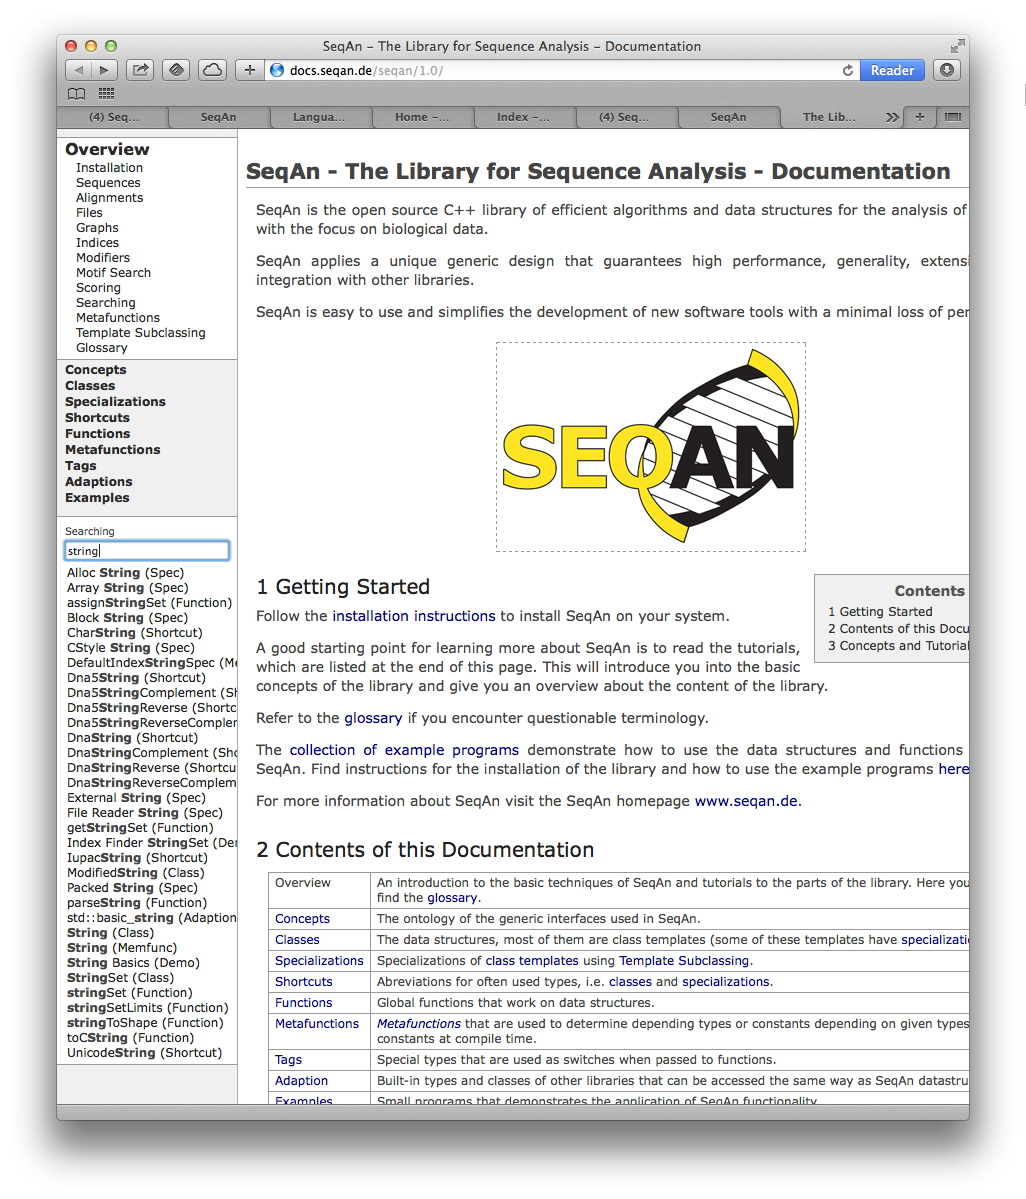
\includegraphics[width=\doxnarrowwidth]{Figures/dox/dox-1_0_0-small-string.png}
    \caption{Seqan-Online-Dokumentation in Version 1.0 - Smale Ansicht - Suche nach ``String''}
    \label{fig:dox-1_0_0-small-string}
\end{figure}

\begin{figure}
  \centering
    \includegraphics[width=\doxnarrowwidth]{Figures/dox/dox-1_4_1-small-string.png}
    \caption{Seqan-Online-Dokumentation in Version 1.4.1 - Smale Ansicht - Suche nach ``String''}
    \label{fig:dox-1_4_1-small-string}
\end{figure}

\begin{figure}
  \centering
    \includegraphics[width=\doxnarrowwidth]{Figures/dox/dox-2_0_0-small-string.png}
    \caption{Seqan-Online-Dokumentation in Version 2.0 - Smale Ansicht - Suche nach ``String''}
    \label{fig:dox-2_0_0-small-string}
\end{figure}

\begin{figure}
  \centering
    \includegraphics[width=\doxnarrowwidth]{Figures/dox/dox-3_0_0-small-string.png}
    \caption{Seqan-Online-Dokumentation in Version 3.0 - Smale Ansicht - Suche nach ``String''}
    \label{fig:dox-3_0_0-small-string}
\end{figure}

Donec urna leo, vulputate vitae porta eu, vehicula blandit libero. Phasellus eget massa et leo condimentum mollis. Nullam molestie, justo at pellentesque vulputate, sapien velit ornare diam, nec gravida lacus augue non diam. Integer mattis lacus id libero ultrices sit amet mollis neque molestie. Integer ut leo eget mi volutpat congue. Vivamus sodales, turpis id venenatis placerat, tellus purus adipiscing magna, eu aliquam nibh dolor id nibh. Pellentesque habitant morbi tristique senectus et netus et malesuada fames ac turpis egestas. Sed cursus convallis quam nec vehicula. Sed vulputate neque eget odio fringilla ac sodales urna feugiat.

Donec urna leo, vulputate vitae porta eu, vehicula blandit libero. Phasellus eget massa et leo condimentum mollis. Nullam molestie, justo at pellentesque vulputate, sapien velit ornare diam, nec gravida lacus augue non diam. Integer mattis lacus id libero ultrices sit amet mollis neque molestie. Integer ut leo eget mi volutpat congue. Vivamus sodales, turpis id venenatis placerat, tellus purus adipiscing magna, eu aliquam nibh dolor id nibh. Pellentesque habitant morbi tristique senectus et netus et malesuada fames ac turpis egestas. Sed cursus convallis quam nec vehicula. Sed vulputate neque eget odio fringilla ac sodales urna feugiat.

\begin{figure}
  \centering
    \includegraphics[width=\doxnarrowwidth]{Figures/dox/dox-1_0_0-small-string-opened.png}
    \caption{Seqan-Online-Dokumentation in Version 1.0 - Smale Ansicht - Klasse ``String''}
    \label{fig:dox-1_0_0-small-string-opened}
\end{figure}

\begin{figure}
  \centering
    \includegraphics[width=\doxnarrowwidth]{Figures/dox/dox-1_4_1-small-string-opened.png}
    \caption{Seqan-Online-Dokumentation in Version 1.4.1 - Smale Ansicht - Klasse ``String''}
    \label{fig:dox-1_4_1-small-string-opened}
\end{figure}

\begin{figure}
  \centering
    \includegraphics[width=\doxnarrowwidth]{Figures/dox/dox-2_0_0-small-string-opened.png}
    \caption{Seqan-Online-Dokumentation in Version 2.0 - Smale Ansicht - Klasse ``String''}
    \label{fig:dox-2_0_0-small-string-opened}
\end{figure}

\begin{figure}
  \centering
    \includegraphics[width=\doxnarrowwidth]{Figures/dox/dox-3_0_0-small-string-opened.png}
    \caption{Seqan-Online-Dokumentation in Version 3.0 - Smale Ansicht - Klasse ``String''}
    \label{fig:dox-3_0_0-small-string-opened}
\end{figure}








Donec urna leo, vulputate vitae porta eu, vehicula blandit libero. Phasellus eget massa et leo condimentum mollis. Nullam molestie, justo at pellentesque vulputate, sapien velit ornare diam, nec gravida lacus augue non diam. Integer mattis lacus id libero ultrices sit amet mollis neque molestie. Integer ut leo eget mi volutpat congue. Vivamus sodales, turpis id venenatis placerat, tellus purus adipiscing magna, eu aliquam nibh dolor id nibh. Pellentesque habitant morbi tristique senectus et netus et malesuada fames ac turpis egestas. Sed cursus convallis quam nec vehicula. Sed vulputate neque eget odio fringilla ac sodales urna feugiat.

\newgeometry{inner=2cm,outer=1.5cm,top=1.5cm,bottom=1.5cm}
\thispagestyle{empty}
\begin{landscape}
\begin{figure}
        \centering
        \begin{subfigure}[b]{0.38\linewidth}
                \includegraphics[width=\linewidth]{Figures/dox/dox-1_0_0-large-home.png}
                \caption{Version 1.0.0}
                \label{fig:dox-large-home-1.0.0}
        \end{subfigure}
        \hspace{1cm}
        \begin{subfigure}[b]{0.38\linewidth}
                \includegraphics[width=\linewidth]{Figures/dox/dox-1_4_1-large-home.png}
                \caption{Version 1.4.1}
                \label{fig:dox-large-home-1.4.1}
        \end{subfigure}%
        \vskip\baselineskip
        \begin{subfigure}[b]{0.38\linewidth}
                \includegraphics[width=\linewidth]{Figures/dox/dox-2_0_0-large-home.png}
                \caption{Version 2.0.0}
                \label{fig:dox-large-home-2.0.0}
        \end{subfigure}
        \hspace{1cm}
        \begin{subfigure}[b]{0.38\linewidth}
                \includegraphics[width=\linewidth]{Figures/dox/dox-3_0_0-large-home.png}
                \caption{Version 3.0.0}
                \label{fig:dox-large-home-3.0.0}
        \end{subfigure}
        \caption{Diese Abbildung zeigt die verschiedenen Online-Dokumentation-Versionen mit ihrer Startseite.}
        \label{fig:dox-large-home-all}
\end{figure}
\end{landscape}
\restoregeometry

\newgeometry{inner=2cm,outer=1cm,top=1.5cm,bottom=1.5cm}
\thispagestyle{empty}
%\begin{landscape}
\begin{figure}
        \centering
        \begin{subfigure}[b]{0.48\linewidth}
                \includegraphics[width=\linewidth]{Figures/dox/dox-1_0_0-small-home.png}
                \caption{Version 1.0.0}
                \label{fig:dox-small-home-1.0.0}
        \end{subfigure}
        \hfill
        \begin{subfigure}[b]{0.48\linewidth}
                \includegraphics[width=\linewidth]{Figures/dox/dox-1_4_1-small-home.png}
                \caption{Version 1.4.1}
                \label{fig:dox-small-home-1.4.1}
        \end{subfigure}%
        \vskip\baselineskip
        \begin{subfigure}[b]{0.48\linewidth}
                \includegraphics[width=\linewidth]{Figures/dox/dox-2_0_0-small-home.png}
                \caption{Version 2.0.0}
                \label{fig:dox-small-home-2.0.0}
        \end{subfigure}
        \hfill
        \begin{subfigure}[b]{0.48\linewidth}
                \includegraphics[width=\linewidth]{Figures/dox/dox-3_0_0-small-home.png}
                \caption{Version 3.0.0}
                \label{fig:dox-small-home-3.0.0}
        \end{subfigure}
        \caption{Diese Abbildung zeigt die verschiedenen Online-Dokumentation-Versionen in schmaler Breiter mit ihrer Startseite.}
        \label{fig:dox-small-home-all}
\end{figure}
%\end{landscape}
\restoregeometry

Donec urna leo, vulputate vitae porta eu, vehicula blandit libero. Phasellus eget massa et leo condimentum mollis. Nullam molestie, justo at pellentesque vulputate, sapien velit ornare diam, nec gravida lacus augue non diam. Integer mattis lacus id libero ultrices sit amet mollis neque molestie. Integer ut leo eget mi volutpat congue. Vivamus sodales, turpis id venenatis placerat, tellus purus adipiscing magna, eu aliquam nibh dolor id nibh. Pellentesque habitant morbi tristique senectus et netus et malesuada fames ac turpis egestas. Sed cursus convallis quam nec vehicula. Sed vulputate neque eget odio fringilla ac sodales urna feugiat.

\newgeometry{inner=2cm,outer=1.5cm,top=1.5cm,bottom=1.5cm}
\thispagestyle{empty}
\begin{landscape}
\begin{figure}
        \centering
        \begin{subfigure}[b]{0.38\linewidth}
                \includegraphics[width=\linewidth]{Figures/dox/dox-1_0_0-large-string.png}
                \caption{Version 1.0.0}
                \label{fig:dox-large-string-1.0.0}
        \end{subfigure}
        \hspace{1cm}
        \begin{subfigure}[b]{0.38\linewidth}
                \includegraphics[width=\linewidth]{Figures/dox/dox-1_4_1-large-string.png}
                \caption{Version 1.4.1}
                \label{fig:dox-large-string-1.4.1}
        \end{subfigure}%
        \vskip\baselineskip
        \begin{subfigure}[b]{0.38\linewidth}
                \includegraphics[width=\linewidth]{Figures/dox/dox-2_0_0-large-string.png}
                \caption{Version 2.0.0}
                \label{fig:dox-large-string-2.0.0}
        \end{subfigure}
        \hspace{1cm}
        \begin{subfigure}[b]{0.38\linewidth}
                \includegraphics[width=\linewidth]{Figures/dox/dox-3_0_0-large-string.png}
                \caption{Version 3.0.0}
                \label{fig:dox-large-string-3.0.0}
        \end{subfigure}
        \caption{Diese Abbildung zeigt die verschiedenen Online-Dokumentation-Versionen mit dem Suchbegriff ``String''.}
        \label{fig:dox-large-string-all}
\end{figure}
\end{landscape}
\restoregeometry

\newgeometry{inner=2cm,outer=1cm,top=1.5cm,bottom=1.5cm}
\thispagestyle{empty}
%\begin{landscape}
\begin{figure}
        \centering
        \begin{subfigure}[b]{0.48\linewidth}
                \includegraphics[width=\linewidth]{Figures/dox/dox-1_0_0-small-string.png}
                \caption{Version 1.0.0}
                \label{fig:dox-small-string-1.0.0}
        \end{subfigure}
        \hfill
        \begin{subfigure}[b]{0.48\linewidth}
                \includegraphics[width=\linewidth]{Figures/dox/dox-1_4_1-small-string.png}
                \caption{Version 1.4.1}
                \label{fig:dox-small-string-1.4.1}
        \end{subfigure}%
        \vskip\baselineskip
        \begin{subfigure}[b]{0.48\linewidth}
                \includegraphics[width=\linewidth]{Figures/dox/dox-2_0_0-small-string.png}
                \caption{Version 2.0.0}
                \label{fig:dox-small-string-2.0.0}
        \end{subfigure}
        \hfill
        \begin{subfigure}[b]{0.48\linewidth}
                \includegraphics[width=\linewidth]{Figures/dox/dox-3_0_0-small-string.png}
                \caption{Version 3.0.0}
                \label{fig:dox-small-string-3.0.0}
        \end{subfigure}
        \caption{Diese Abbildung zeigt die verschiedenen Online-Dokumentation-Versionen in schmaler Breiter mit dem Suchbegriff ``String''.}
        \label{fig:dox-small-string-all}
\end{figure}
%\end{landscape}
\restoregeometry

Donec urna leo, vulputate vitae porta eu, vehicula blandit libero. Phasellus eget massa et leo condimentum mollis. Nullam molestie, justo at pellentesque vulputate, sapien velit ornare diam, nec gravida lacus augue non diam. Integer mattis lacus id libero ultrices sit amet mollis neque molestie. Integer ut leo eget mi volutpat congue. Vivamus sodales, turpis id venenatis placerat, tellus purus adipiscing magna, eu aliquam nibh dolor id nibh. Pellentesque habitant morbi tristique senectus et netus et malesuada fames ac turpis egestas. Sed cursus convallis quam nec vehicula. Sed vulputate neque eget odio fringilla ac sodales urna feugiat.

\newgeometry{inner=2cm,outer=1.5cm,top=1.5cm,bottom=1.5cm}
\thispagestyle{empty}
\begin{landscape}
\begin{figure}
        \centering
        \begin{subfigure}[b]{0.38\linewidth}
                \includegraphics[width=\linewidth]{Figures/dox/dox-1_0_0-large-string-opened.png}
                \caption{Version 1.0.0}
                \label{fig:dox-large-string-opened-1.0.0}
        \end{subfigure}
        \hspace{1cm}
        \begin{subfigure}[b]{0.38\linewidth}
                \includegraphics[width=\linewidth]{Figures/dox/dox-1_4_1-large-string-opened.png}
                \caption{Version 1.4.1}
                \label{fig:dox-large-string-opened-1.4.1}
        \end{subfigure}%
        \vskip\baselineskip
        \begin{subfigure}[b]{0.38\linewidth}
                \includegraphics[width=\linewidth]{Figures/dox/dox-2_0_0-large-string-opened.png}
                \caption{Version 2.0.0}
                \label{fig:dox-large-string-opened-2.0.0}
        \end{subfigure}
        \hspace{1cm}
        \begin{subfigure}[b]{0.38\linewidth}
                \includegraphics[width=\linewidth]{Figures/dox/dox-3_0_0-large-string-opened.png}
                \caption{Version 3.0.0}
                \label{fig:dox-large-string-opened-3.0.0}
        \end{subfigure}
        \caption{Diese Abbildung zeigt die verschiedenen Online-Dokumentation-Versionen mit der geöffneten Klasse \textit{String}.}
        \label{fig:dox-large-string-opened-all}
\end{figure}
\end{landscape}
\restoregeometry

\newgeometry{inner=2cm,outer=1cm,top=1.5cm,bottom=1.5cm}
\thispagestyle{empty}
%\begin{landscape}
\begin{figure}
        \centering
        \begin{subfigure}[b]{0.48\linewidth}
                \includegraphics[width=\linewidth]{Figures/dox/dox-1_0_0-small-string-opened.png}
                \caption{Version 1.0.0}
                \label{fig:dox-small-string-opened-1.0.0}
        \end{subfigure}
        \hfill
        \begin{subfigure}[b]{0.48\linewidth}
                \includegraphics[width=\linewidth]{Figures/dox/dox-1_4_1-small-string-opened.png}
                \caption{Version 1.4.1}
                \label{fig:dox-small-string-opened-1.4.1}
        \end{subfigure}%
        \vskip\baselineskip
        \begin{subfigure}[b]{0.48\linewidth}
                \includegraphics[width=\linewidth]{Figures/dox/dox-2_0_0-small-string-opened.png}
                \caption{Version 2.0.0}
                \label{fig:dox-small-string-opened-2.0.0}
        \end{subfigure}
        \hfill
        \begin{subfigure}[b]{0.48\linewidth}
                \includegraphics[width=\linewidth]{Figures/dox/dox-3_0_0-small-string-opened.png}
                \caption{Version 3.0.0}
                \label{fig:dox-small-string-opened-3.0.0}
        \end{subfigure}
        \caption{Diese Abbildung zeigt die verschiedenen Online-Dokumentation-Versionen in schmaler Breiter mit der geöffneten Klasse \textit{String}.}
        \label{fig:dox-small-string-opened-all}
\end{figure}
%\end{landscape}
\restoregeometry
\end{comment}


\subsection{Kollaborationsplattform}

Im Zuge der Umstellung des Versionsverwaltungssystems von Subversion auf Git wurde von einer selbst gehosteten Lösung auf \textit{GitHub}\footnote{\url{https://github.com}} umgestellt. Diese Plattform bietet einen \textit{Issue-Tracker}\footnote{\url{https://github.com/seqan/seqan/issues}}, der von SeqAn-Anwendern sehr gut angenommen und von SeqAn-Entwicklern aktiv verwaltet wird. Auf dieser Plattform findet ein fruchtbarer Austausch zwischen Anwendern und Entwicklern statt\footnote{Beispiel: \url{https://github.com/seqan/seqan/issues/919}}. 


\begin{comment}
\subsection{Werkzeugunterstützung}

Den Algorithmus zur automatischen Erzeugung von Code-Beispielen von \cite{Buse:2012vv} habe ich aus Zeitgründen nicht den SeqAn-Entwicklern vorstellig machen können.
\end{comment}



\subsection{Usability-Priorisierung}

Die gesamtheitliche Erforschung der Entwicklung der SeqAn-Library brachte erst spät die trivial erscheinende Erkenntnis, dass es Gründe für die besondere Betonung der Performance gab und erst die kommerzielle Verbreiterung des SeqAn-Einsatzzweckes zu einer notwendigen Neugewichtung der Usability führt bzw. führen muss.

Mit dieser Arbeit liefere ich belastbare Argumente für meine Theorie, die dem SeqAn-Entwicklungsteam dabei helfen sollen, diesen Perspektivwechsel wahrzunehmen und eine verstärkte Betonung der Usability in Form von expliziten-empirischen Entwurfsentscheidungen zu fördern. Diese Einsicht auf Entwicklerseite würde mittelfristig zu einer ganzheitlichen Verbesserung der API-Usability von SeqAn führen.



\subsection{Zusammenfassung}

Für die Verbesserung der API-Usability von SeqAn haben die Bioinformatik-Arbeitsgruppe und ich umfangreiche Maßnahmen umgesetzt.

Neben den aus der ersten Verbesserungsiteration stammenden Prozessverbesserungen, konnten meine SeqAn-Kollegen und ich drei der vier wichtigsten Maßnahmen vollständig bearbeiten:
\begin{enumerate}
  \item SeqAn kann nun auch als Library verwendet werden, indem insbesondere Vorwärtsdeklarationen beseitigt wurden. So simpel dieser Punkt klingen mag, so fundamental war er auch für potentielle SeqAn-Anwender, die ihren bestehenden Build-Prozess nicht anpassen wollten oder konnten. 
  \item Die Dokumentation wurde technisch neu entwickelt und inhaltlich überarbeitet. Dazu wurde das neue Dokumentationsformat Dox entwickelt, ein Gesamtüberblick erarbeitet sowie Seitenaufbau, Beispiele, Suchfunktion, Darstellung und die Integration verbessert. Außerdem wurde das Konzept der Sprachentitätstypen gesamtheitlich innerhalb der Dokumentation implementiert. Ergänzt wird die Verbesserung der Dokumentation durch die bereits in der ersten Verbesserungsiteration generalüberholten Installationsanleitungen und Tutorials.
  \item SeqAn kann nun von API-Endanwendern genutzt werden. Dazu wurde eine Wrapper-API in Form einer Integration in die Workflow-Engine KNIME implementiert.% Zu diesem Zweck wurde ein neuer Argument-Parser entwickelt, der explizierte Schnittstellenbeschreibungen von SeqAn-Anwendungen in einem definierten Format ausgeben kann. Diese Beschreibungen dienen wiederum dem ebenfalls weiterentwickelten Generic Workflows Nodes Werkzeug als Eingabe zur Generierung von KNIME-Knoten, die ein automatisierter Prozess allen KNIME-Anwendern zur Verfügung stellt. 
\end{enumerate}

Außerdem abgeschlossen wurde die Einrichtung einer Kollaborationsplattform --- in Form eines GitHub Issue-Trackers --- für den Austausch zwischen SeqAn-Entwicklern und -Anwendern.

Aus diversen, insbesondere Zeitgründen konnte ich leider nicht darauf hinwirken, dass die wichtige STL-Angleichung in Angriff genommen wurde. Zwar sind Metafunktionen zur Berechnung von Rückgabetypen, wegen des in C\texttt{++}11 eingeführten \texttt{auto}-Schlüsselworts theoretisch nicht mehr nötig, was die mit dieser Maßnahme in Verbindung stehenden Usability-Probleme teilweise entschärft. Dies muss jedoch noch praktisch gezeigt werden. Im Erfolgsfall müssen außerdem sämtliche Lernressourcen entsprechend angepasst werden. Diese Entwicklung hat jedoch keinen Einfluss auf meine dringende Empfehlung, das CRTP einzusetzen, um die globalen Funktionen zu Memberfunktionen zu refaktorisieren, die auch in C\texttt{++} als Memberfunktionen implementiert sind.

Ebenfalls aus Zeitgründen konnten die Maßnahmen Inkonsistenzbeseitigung, Shortcuts und die Evaluation des Code-Beispiel-Erzeugungs-Algorithmus nicht umgesetzt werden.

Das dem der Maßnahme Intransparenzbeseitigung zu Grunde liegende Usability-Problem \code[apiua://code/-9223372036854775057]{versteckte Parameterübergabe} ist in Bezug auf seine Fatalität nicht hinreichend gut verstanden, weshalb ich die Umsetzung der Maßnahme angesichts der hohen Kosten momentan nicht empfehlen kann.

Die Umsetzung der abstrakten Maßnahme Usability-Priorisierung ist längst nicht abgeschlossen und soll durch diese Arbeit motiviert werden.